\documentclass[a4j,12pt,onecolumn]{ujarticle} % jsbook, jsreportなど

%% マージン等の設定
%% A4: 210 x 297 mm
%% jsクラスではフォントサイズを10ptから変更するときには長さ単位にtrueをつける必要がある.
%% inch->trueinch, mm->truemm, cm->truecmなど.
\setlength{\textwidth}{15truecm}       %% 150mm + 1inch(25.4mm)*2 + 4.6mm*2 = 210mm
\setlength{\oddsidemargin}{4.6truemm}  %% 左右余白30mm
\setlength{\evensidemargin}{4.6truemm}
\setlength{\textheight}{227truemm} %% 227mm + 1inch*2 + 9.6mm*2 = 297mm
\setlength{\headheight}{9.6truemm} %% 上下余白35mm
\setlength{\topmargin}{9.6truemm}
\setlength{\headsep}{-15truemm}
%% 代わりに以下2行でもOK
%% \usepackage{geometry}
%% \geometry{top=35truemm,bottom=35truemm,left=30truemm,right=30truemm}

%% \renewcommand{\baselinestretch}{0.82}

%% 使いたいパッケージを指定
\usepackage[dvipdfmx]{graphicx, color} % 画像挿入
\usepackage{styles/mediabb} % PDFなどのbounding boxを取得してくれる
\usepackage{amsmath} % 数式用パッケージ
\usepackage{url} % URL挿入用
\usepackage{color} % 文字色指定
\usepackage{bm} % bold math (数式中のベクトルなどで太字にしたいとき)

%% マクロ(ユーザ定義命令)を宣言
\newcommand{\hoge}{\textcolor{red}{ほげほげ}}    % 引数なし
\newcommand{\Hoge}[2]{\textcolor{#1}{#2#2}}      % 引数あり
\newcommand{\HOGE}[2][red]{\textcolor{#1}{#2#2}} % 引数あり(オプション引数付き)

\title{ 自動チューニング化手法 }
\author{井上裕太}
\date{\today}

%% --- 以下本文 ---
\begin{document}
\maketitle %% タイトルを表示

% \chapter{チャプター}
% jsarticleには\verb+\chapter+命令がない.

%% 目次作成
\tableofcontents
\listoffigures
\listoftables

% \section{序論}
\subsection{研究の背景}
脳機能の理解を目的として,スーパコンピュータを用いた神経回路のシミュレーションが行われている. また,消費電力やシミュレーションの割り当て時間といったリソースの問題やリアルタイムデータ同化への需要から
シミュレーションの高速化・最適化が求められている. しかし,神経細胞には様々な種類のものが存在するため,個々の神経細胞のイオンチャンネルのモデルを最適化された形で実装するために,これまでそれぞれのモデルに対して多大な努力が行われてきた.
また,現代の計算機にも多様な種類が存在し,それぞれに対する最適化も個別に行われてきた.
本研究の目的はそれぞれの細胞モデルのシミュレーションコードを個々のアーキテクチャに合わせて,自動又は半自動的に最適化を行う手法を確立することである.

\subsection{研究の目的と手法}
通常はソース内で
何回改行しようと
このように
出力
結果で改行は
起こらない.
改行するには\\
\verb+\+\verb+\+や\verb+\newline+を用いる.

また,このようにソースで一行空けると
改段落が発生する.自動的に字下げされているよね.\verb+\par+でも同じ.\par
字下げを明示的に指定するには\verb+\indent+や\verb+\noindent+を使う.

\noindent このようにインデントが抑制される.

\verb+\newpage+をというコマンドもあり,使うと{\newpage}こうなる.

\subsection{本論文の構成}
本論文は全5章から構成される.
本章では本研究の背景・目的について述べた.
第2章では,実験方法について述べる.

\section{序論}
\subsection{神経科学においてシミュレーションを行う意義}
脳機能の理解を目的として,スーパコンピュータを用いた神経回路のシミュレーションが行われている.
また,消費電力やシミュレーションの割り当て時間といったリソースの問題やリアルタイムデータ同化への
需要からシミュレーションの高速化・最適化が求められている.
しかし,神経細胞には様々な種類のものが存在するため,
個々の神経細胞のイオンチャンネルのモデルを最適化された形で実装するために,
これまでそれぞれのモデルに対して多大な努力が行われてきた.
また,現代の計算機にも多様な種類が存在し,それぞれに対する最適化も個別に行われてきた.
本研究の目的はそれぞれの細胞モデルのシミュレーションコードを個々のアーキテクチャに合わせて,
自動又は半自動的に最適化を行う手法を確立することである.

\subsection{神経回路シミュレーションの高速化・最適化への需要}

\subsection{先行研究}
\subsubsection{宮本さんの}
脳機能の理解を目的として,スーパコンピュータを用いた神経回路のシミュレーションが行われている.
また,消費電力やシミュレーションの割り当て時間といったリソースの問題やリアルタイムデータ同化への
需要からシミュレーションの高速化・最適化が求められている.
しかし,神経細胞には様々な種類のものが存在するため,
個々の神経細胞のイオンチャンネルのモデルを最適化された形で実装するために,
これまでそれぞれのモデルに対して多大な努力が行われてきた.
また,現代の計算機にも多様な種類が存在し,それぞれに対する最適化も個別に行われてきた.
本研究の目的はそれぞれの細胞モデルのシミュレーションコードを個々のアーキテクチャに合わせて,
自動又は半自動的に最適化を行う手法を確立することである.

\subsubsection{片桐先生の}

\subsection{研究の目的と手法}
以上のことを踏まえ, 本研究の目的は,
\begin{enumerate}
\item NEURON上でのシミュレーションを自動で最適化するために, 最適化に用いることのできるパラメータの候補を,
パラメータを定義した設定ファイルをパースすることまたはMODファイルやマシンを解析することによって生成する.
\item 与えられた最適化のパラメータを用いて, MODファイルから最適化されたC言語ファイルを生成するトランスパイラを作成する.
\item 1で生成したパラメータ候補に対し, 2を利用してC言語ファイルを生成し, シミュレーションの実行とシミュレーションの結果を自動で行うシミュレータを作成する.
\end{enumerate}
の3点とする.

\subsection{本論文の構成}
以上が本研究の背景と動機である. この問題意識のもと,\\
\indent 第2章では,本研究が対象とする神経回路シミュレーションの系,そしてシミュレーションを行う環境について述べる.\\
\indent 続く第3章では,本研究で作成したプログラムのアルゴリズムについて述べる.\\
\indent そして第4章では,本研究で作成したプログラムについての詳細を述べる.\\
\indent 第5章では,シミュレーションの結果を示し,
\indent 第6章では,シミュレーション結果の考察を述べる.\\
\indent 最後に第7章では,本研究のまとめ,成果を示した上で将来の課題について述べる.\\


\section{シミュレーションモデル}
% シミュレーションを行ったモデル
\subsection{Hodgkin Huxleyモデル}
\subsection{Purkinje Cellモデル}
\subsection{ベンチマークモデル}


\section{シミュレーション環境}
% シミュレーションを行う環境について
\subsection{京コンピュータ}
\subsubsection{CPUアーキテクチャ}
\subsubsection{キャッシュ・メモリ}
\subsection{研究室クラスタ}
\subsubsection{CPUアーキテクチャ}
\subsubsection{キャッシュ・メモリ}


\section{最適化の手法}
% 最適化のアルゴリズム・注目した点について
本研究では,モデルに依存するパラメータと実行マシンに依存するパラメータ,そしてプログラムのコンパイル時に関わるパラメータ(コンパイルオプション)を調節することでシミュレーション系の最適化を目指した.\\
以下にそれぞれのパラメータの詳細を示す.\\
\subsection{モデルに依存するパラメータ}
以下にHodgkin-Huxley方程式のモデルを例としてそれぞれのパラメータを示す.\\
モデルに依存するパラメータに関しては先行研究 ( TODO: add reference)においてSIMD化, 配列構造の最適化により計算速度が大きく向上することが示されているため,
その二つに加え配列構造の順序を入れ替えることによってキャッシュヒット率の向上に取り組んだ.\\
Hodgkin-Huxley方程式は,NEURON内においてMOD形式で次のように記述されている.\\
{\footnotesize
\lstinputlisting[caption=aaa,label=hogehoge,frame=single]{src/mod/hh.mod}
}
先行研究の中でも示されている通り,この中でプロファイル結果から多くの計算時間を必要とするのはDERIVATIVE ( TODO: reference)
であり以下のパラメータの多くはDERIVATIVEの計算を行う上でキャッシュヒット率をあげることを目的としている.\\
\subsubsection{SIMD化}
・宮本さんの論文を参照
また,SIMD化を行う方法としてavxやinline asmなどを利用する方法も存在する.\\
これは現在の課題である汎用性を達成した上で,汎用性を崩さないよう取り組む内容であるため,
今後の課題としたい.\\

・変数の配列化によるメモリアクセスの連続化
\subsubsection{配列構造}
( TODO: 例)配列を複数定義し,一つの計算の中で呼び出す場合,Array of Structureでなく
Structure of Arrayとして定義した方が計算が高速化される場合がある.\\
これは以下に示す図によるものである\\
( TODO: 図)
一方で,一つの構造体に多くの変数を定義してしまうとキャッシュラインに入らず,
結果としてキャッシュミスを多発し逆に遅くなるといった問題が生じる.\\
そこで,MODファイル内で定義された計算式の中から変数を抜き出し,
それぞれの変数をUnion-Find木 ( TODO : reference)を用いてグループにまとめ構造体として利用する変数の候補とし,
それぞれの構造体を使うか否かでの高速化を図る.\\
Union-Find木を用いているため,キャッシュという観点ではグループ間の関連はないと言えるため,
これらのグループは独立にシミュレーションを行うことができる.\\
よって,仮に変数のグループがn個できた場合でも2n回の試行を行うことで最適な組み合わせを見つけることができる.
( TODO: SOAの論文を引用)

・配列の構造変形(時間があれば)なければここを消す
\subsection{実行マシンに依存するパラメータ}
近年のCPUはシングルコアではなく,マルチコアによって計算を並列化することで全体としての計算能力を向上させている.\\
一方で,この並列化を行う上でのパラメータは実行するマシンごとに依存するものである.\\
ここで主に対象としたパラメータはOpenMPのスレッド数とMPIのプロセス数である.\\
\subsubsection{スレッド数}
OpenMPのスレッドに関与するパラメータに関する説明 ( TODO : わあああ)
\subsubsection{プロセス数}
MPIプロセスに関与するパラメータに関する説明 ( TODO : わあああい)
\subsubsection{配列サイズの変形}
\subsubsection{配列サイズの変形}

\subsection{コンパイルに関わるパラメータ}
TODO: 時間があれば記述する


\section{自動チューニングスクリプトとMODトランスパイラの構築}
% 手法をどう実現したかの説明
本研究では環境・イオンチャンネルモデルに関わらない自動最適化を目的としている.\\
そのため,スーパーコンピュータ京・研究室クラスタ以外のマシンを用いる場合においても環境構築,プログラムの修正・実行にかかるコストは最小限になるべきである.\\
上記の要件を満たすため,以下にあげる3種類のプログラムを作成した.\\
また,それぞれのプログラムはPython, Shell Script( TODO: reference)を使用して作成している.\\
\subsection{環境設定スクリプト}
% 環境設定に関わるスクリプトの説明(研究室クラスタ, 京に対する)
作成したシミュレータ・トランスパイラはPython( TODO: reference)のモジュールとして作成したが,
pip( TODO: reference )のようなモジュール管理ツールが存在しない環境(スーパーコンピュータ京)においては,
モジュールとして公開するだけでは不十分である.\\
特にスーパーコンピュータ京では,デフォルトのPython( TODO: reference)のバージョンが2.6.6,
sudo権限を有しないため外部プログラムのインストールが難しいという環境であったため,
Pyenvを利用して汎用的な環境を作成することにした.\\


% パラメータ推定をするためのシミュレーションを実行する環境のためのシミュレータの説明
最適化の方法として,複数のパラメータからモデル,実行環境に即したパラメータを選択するという手法を選択したが,
そのためには複数のパラメータでシミュレーションを行いその結果を集約するプログラムが必要となる.\\
本研究ではこのパラメータ選択を容易かつ高速に行うため以下に示すプログラムを作成した.\\
・MODファイルからパラメータとなりうる変数を自動で抽出し,それぞれの関係性を元に配列とその順序の候補を生成する.\\
・ジョブキューのシステムを持っているマシンにおいて,複数のジョブを並行して投げ結果を非同期的に集約できる.\\
・実行結果を最適化前のデフォルトの結果と比較し,実行結果に対して影響がないかを確認する.\\
・json形式で実行するファイル,各パラメータの範囲(プロセス数は1から10など)を指定することができる.\\
\subsubsection{全体構成}
はじめにシミュレータプログラムを構成する要素について示す.\\
( TODO: 章番号)にあるアルゴリズムで述べたように,探索の対象となるパラメータは,モデルに依存するパラメータ,
実行マシンに依存するパラメータそしてコンパイルに関わるパラメータの3つに大別される.\\
そのうち,モデルとコンパイルに関わるパラメータは実行形式の生成に関与し,実行マシンに関わるパラメータは
ジョブスクリプトの生成に関わる.\\
\paragraph{単一ジョブの実行}
パラメータのシミュレーションを一度行う際のプログラムの動作を次に示す.\\
\begin{figure}[htb]
% h:here, t:top, b:bottom, p:page
  \begin{center}
    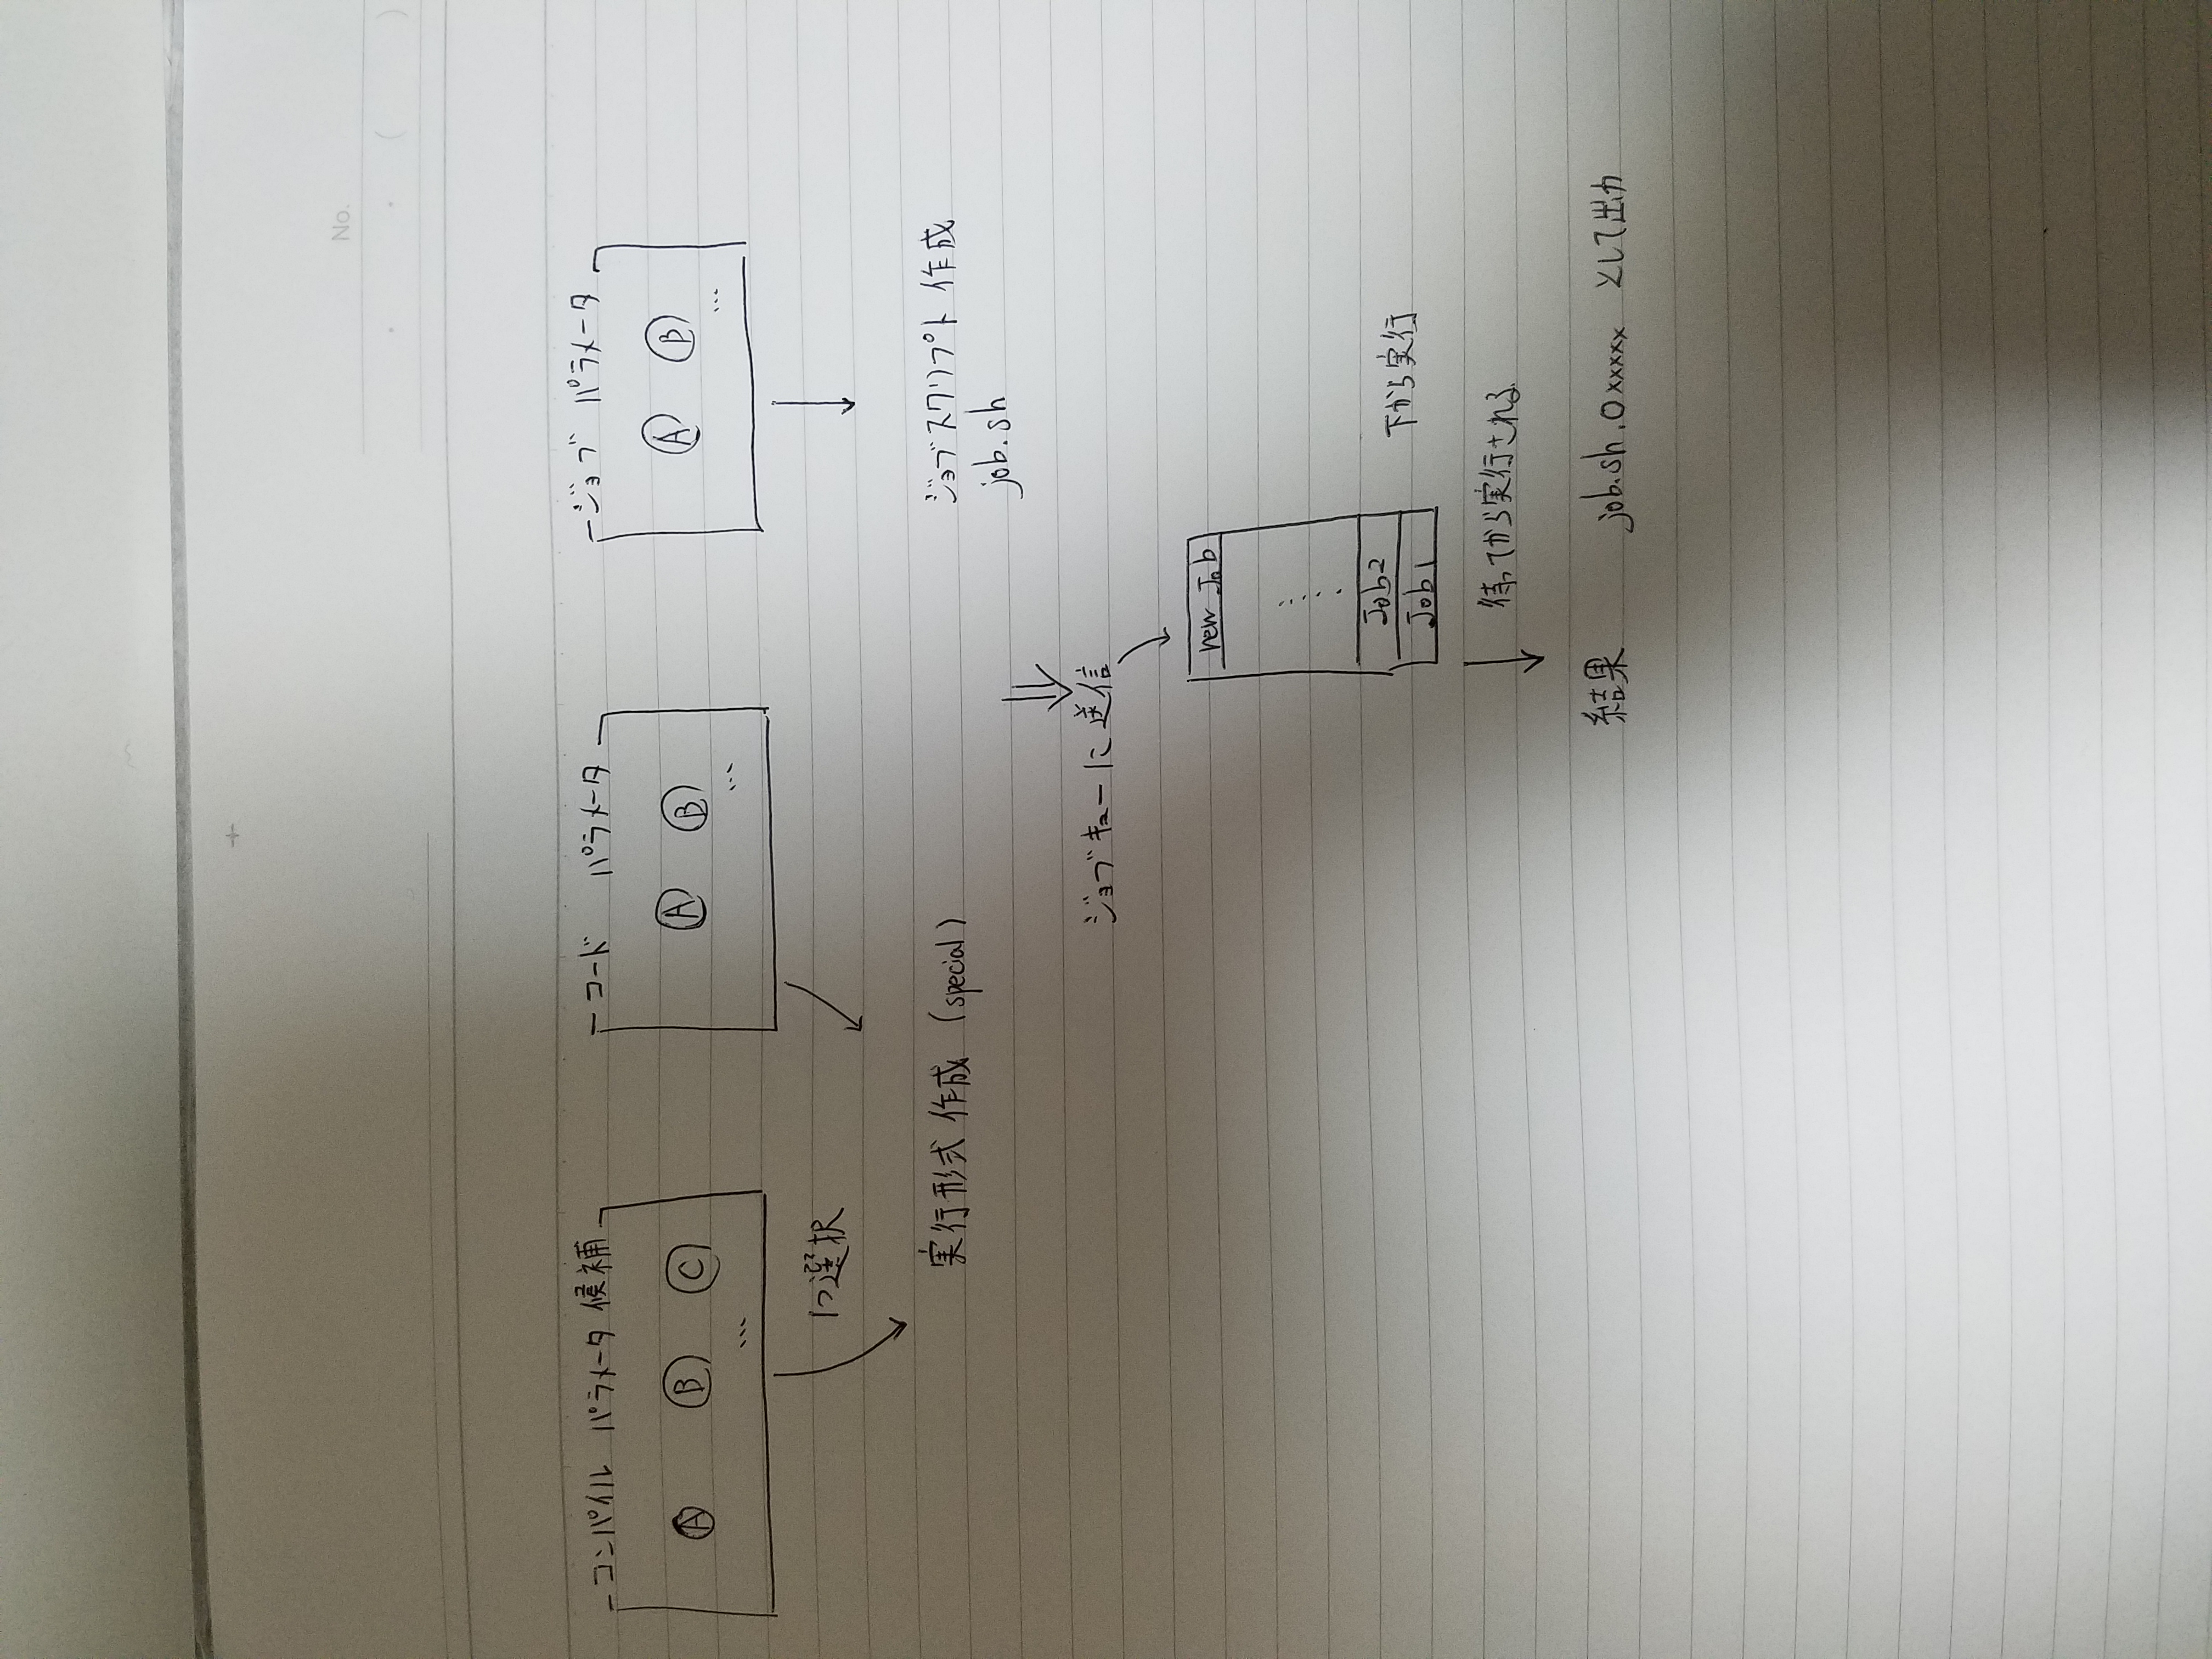
\includegraphics[width=10.0cm]{./images/singlejob}
    \caption{単一ジョブ実行時の挙動}
    \label{fig:singlejob}
  \end{center}
\end{figure}
\\
図( TODO: 番号)にあるようにジョブの実行はジョブの生成,ジョブの実行,ジョブ結果の集約の3段階に分かれており,
ジョブの生成にかかる時間そしてジョブが実行されるまでのジョブキューでの待機時間がこの一連の動作の実行時間において大きな割合を示す.\\
ジョブが実行されるまでの待機時間は複数のジョブを実行する場合ではジョブの実行時間と同義になるため,これはシミュレーションの内容に応じて変わるが,
ジョブの生成に関してはビルドするプログラムに大きな違いは現れず,多くの場合ジョブの生成時間 $<$ ジョブの実行時間という関係が成立する.\\

また,ジョブの生成部分について詳しく見ると,実行形式とジョブスクリプトそれぞれの生成にかかる時間は表 ( TODO: 表を作る)のようになり,
スーパーコンピュータ京,研究室クラスタ双方において実行形式の生成にかかる時間が多いことがわかる.\\

\paragraph{複数ジョブの並列実行}
次にシミュレータの詳細について複数のジョブの並列実行を例として示す.\\

単一ジョブの実行例からパラメータを選択するためにコード,コンパイル,ジョブそれぞれの候補から一つを選択するという3重のループを組む際に,
最も内側のループ内でジョブスクリプトの生成を行い,外側のループで生成した実行形式を使い回すことでシミュレーションをより高速に行うことができる.\\
また,スーパーコンピュータ京のように非常に多くのノードを持つマシンでない場合,ジョブの実行時間の方が長いため多数のジョブがジョブキューに溜まる状態になる.
そのため,外側のループで実行形式を生成する形を取ることで,ジョブの実行が溜まっているうちに実行形式のビルドを行うことができるようになり,結果として最初の一回を除き以降のビルドは
シミュレーションの実行時間に関与しなくすることができる.\\

本研究では以上を念頭に置きシミュレータのプログラムを作成した.\\
単一ジョブの実行 ( TODO: add ref)で述べたように,ジョブの実行をするにはジョブの生成,ジョブの実行,ジョブ結果の集約が必要となる.\\
その中でジョブの実行はqsubやpjsubといった環境にインストールされているジョブ実行環境を利用するため,シミュレータはジョブの生成と結果の集約の役割を担う.\\
\begin{figure}[htb]
% h:here, t:top, b:bottom, p:page
  \begin{center}
    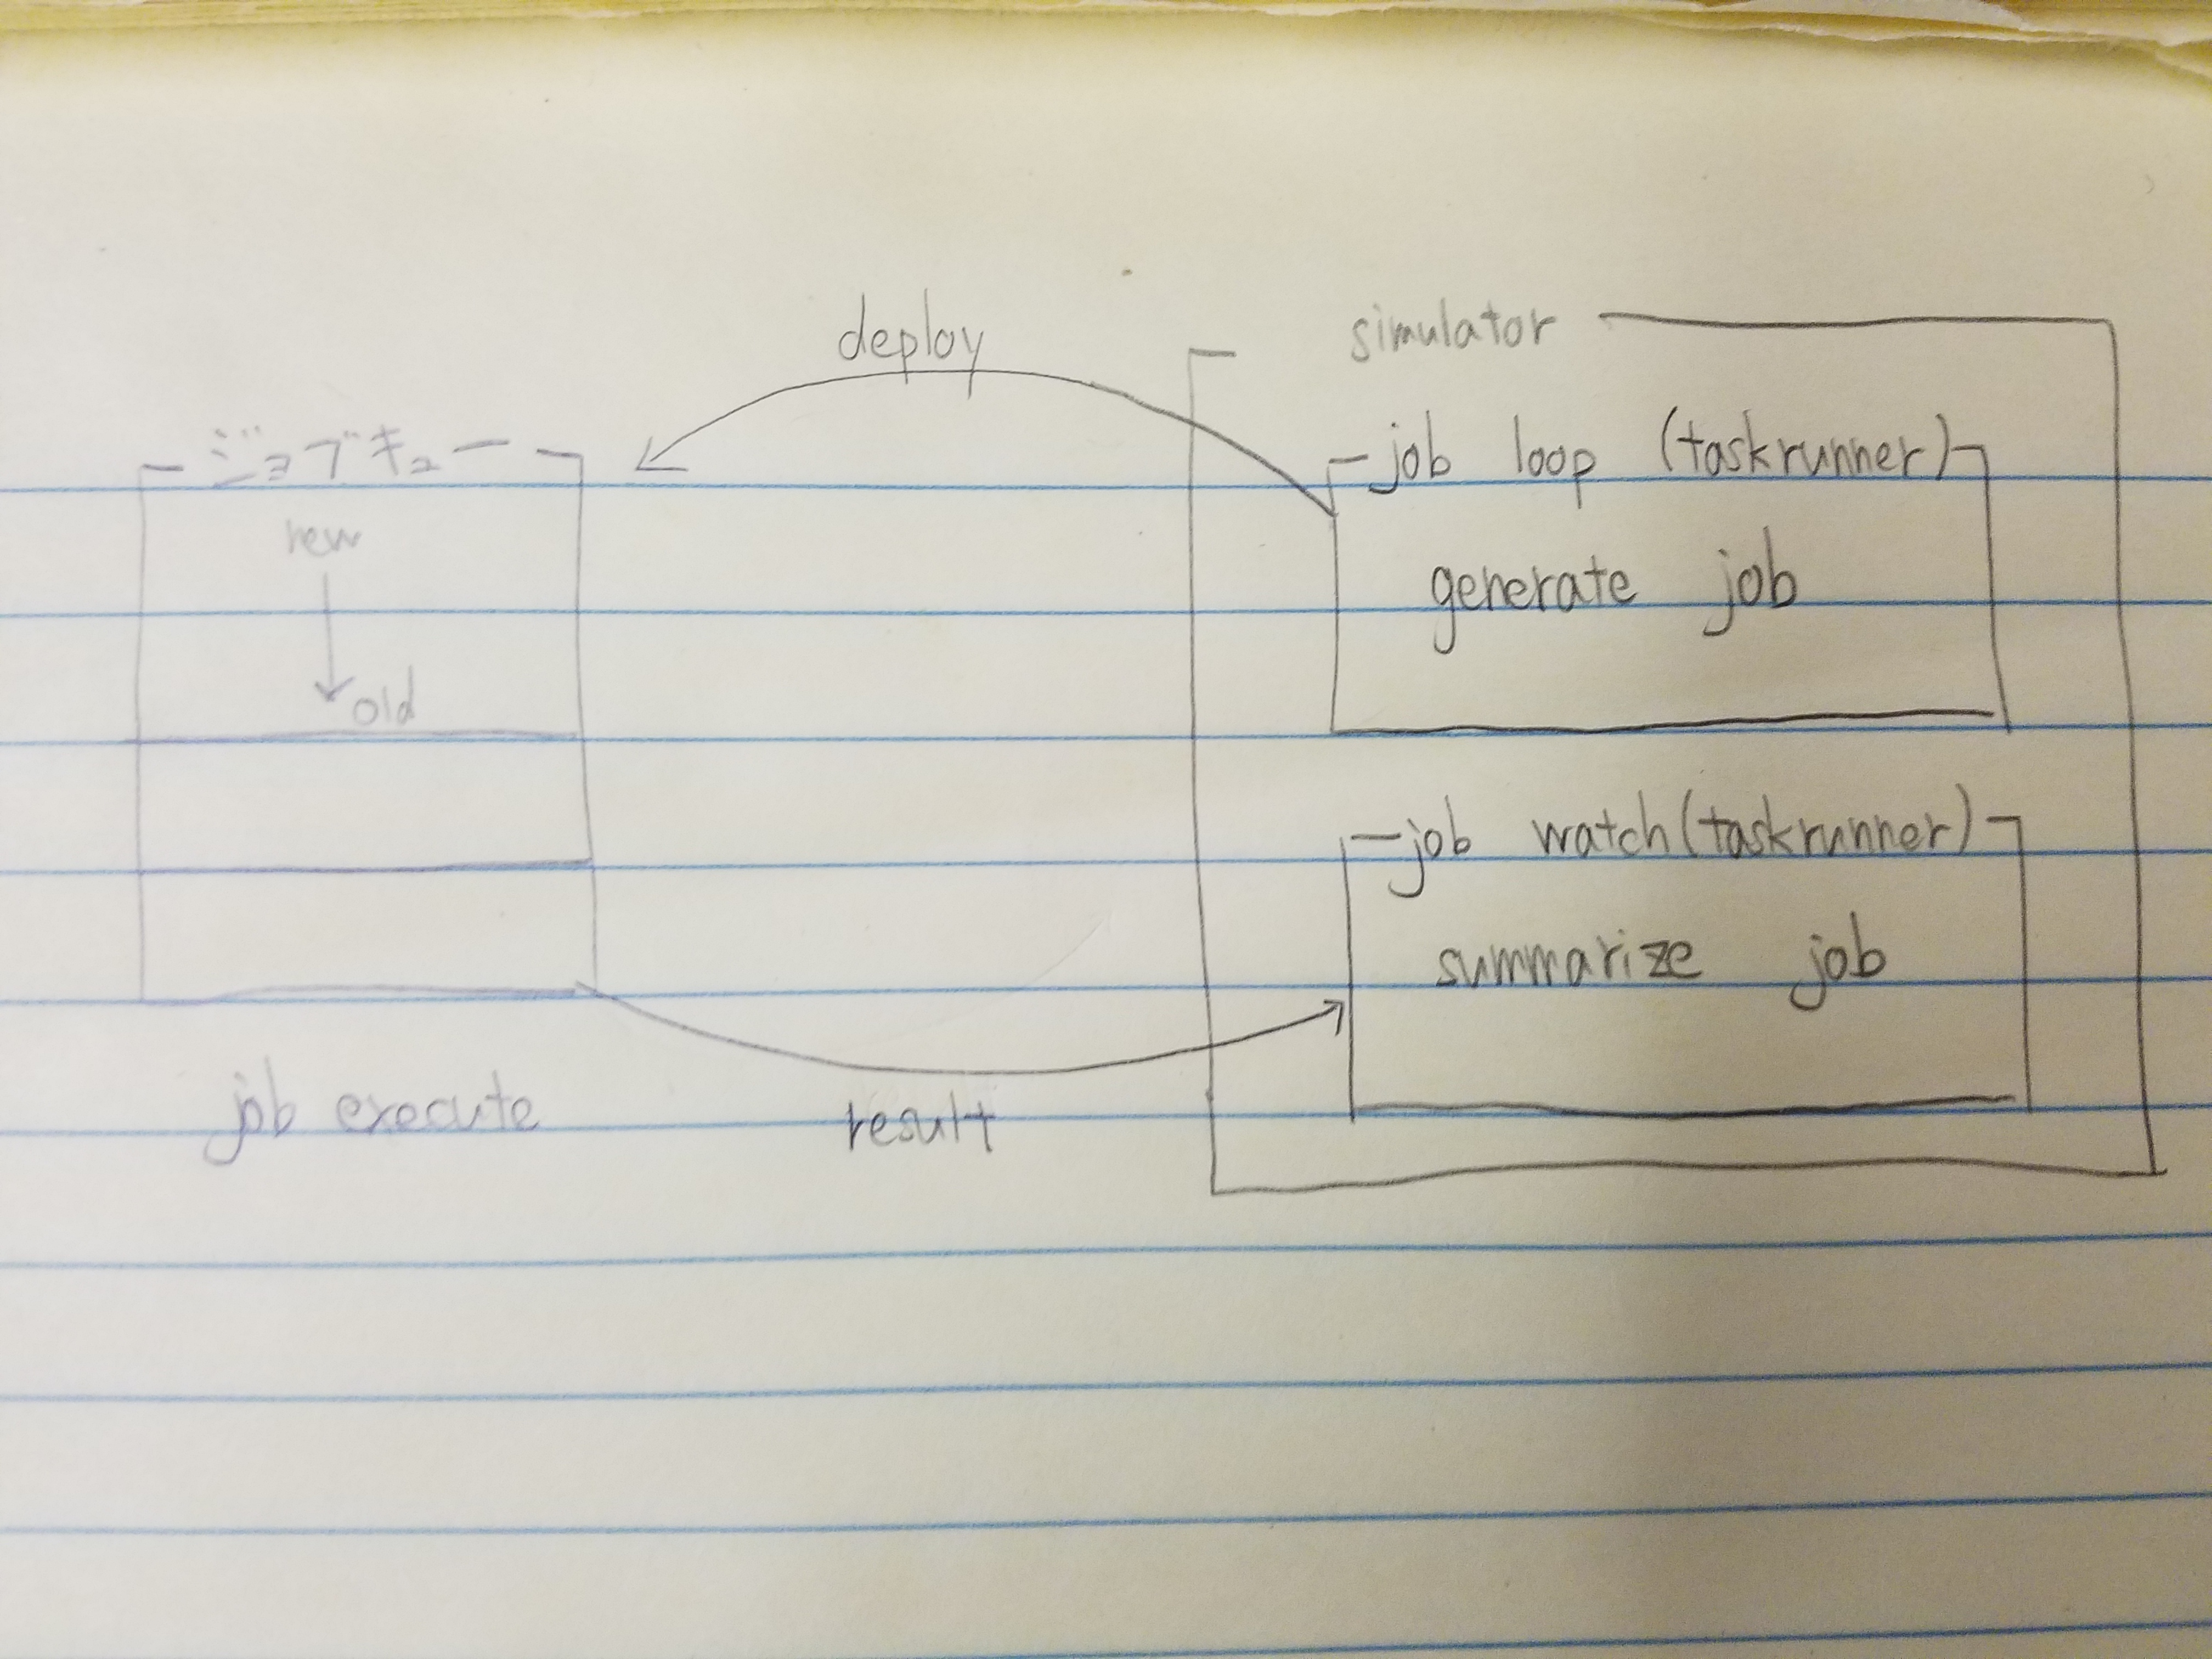
\includegraphics[width=10.0cm]{./images/simulator.pdf}
    \caption{シミュレータ 構成}
    \label{fig:test}
  \end{center}
\end{figure}
\\
そのため,シミュレータは次の疑似コードで示す通りジョブを生成するためのループと
メインスレッドから切り離されたスレッドでジョブの実行状況を監視し,
ジョブが終了したタイミングで結果の集約を行うメソッドという二つの機能から成り立っている.\\
\\
\\
\\
\\
\\
\\
\\
\\
\\
{\footnotesize
\lstinputlisting[caption=シミュレータ疑似コード,label=pseudocode-simulator,frame=single]{src/pseudocode/simulator}
}
また疑似コードを状態遷移図の形で可視化したものが次になる.\\
\begin{figure}[htb]
% h:here, t:top, b:bottom, p:page
  \begin{center}
    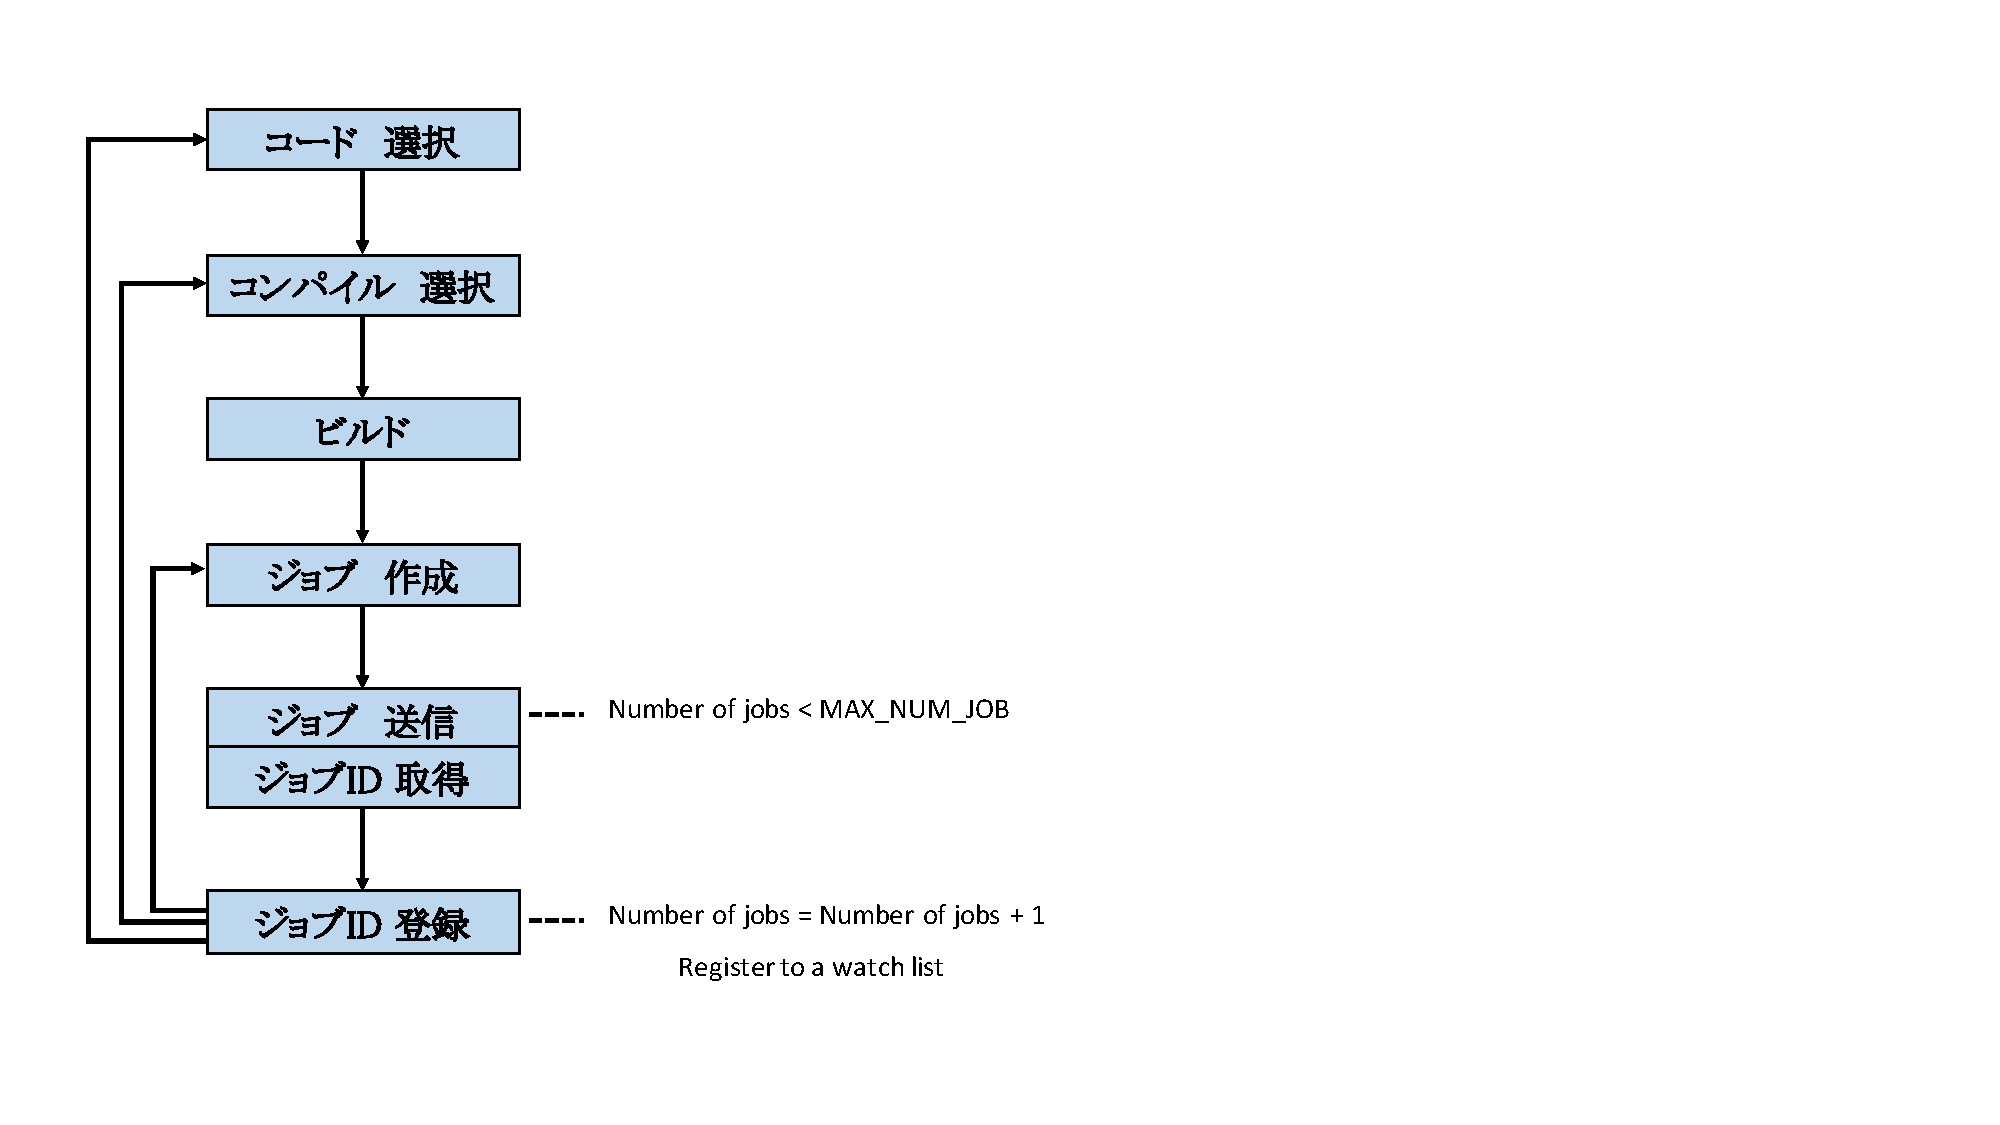
\includegraphics[width=20.0cm]{./images/state.pdf}
    \caption{シミュレータ 状態遷移図}
    \label{fig:test}
  \end{center}
\end{figure}
\subparagraph{ジョブ生成ループ}~\\
疑似コード内の8-22行目までがジョブ生成のためのループを構成している.\\
{\footnotesize
\lstinputlisting[caption=シミュレータ ジョブ生成ループ,label=pseudocode-simulator-job-gen-loop,frame=single, firstline=8, lastline=22]{src/pseudocode/simulator}
}
ループ内部では,プログラムのビルド,ジョブスクリプトの生成,そして生成した実行形式とジョブスクリプトをジョブキューにdeployするという3つのことを行っている.\\
すでに ( TODO: add re)で述べたようにパラメータ候補の選択順を実効形式の生成に関わるものを先にすることで,非同期的に実行形式の生成とジョブの実行を行うことができる.\\
\\
\subparagraph{ジョブ実行}~\\
{\footnotesize
\lstinputlisting[caption=シミュレータ ジョブ実行,label=pseudocode-simulator-job-deploy,frame=single, firstline=24, lastline=29]{src/pseudocode/simulator}
}
スーパーコンピュータ京のような複数のユーザーが用いるシステムにおいて,ジョブを一度に大量に投げるのは好ましくない.\\
そのため,ジョブをジョブキューに投げる前に事前に設定した最大同時ジョブ実行数と現在の実行中のジョブの数を比較し,最大数と同数なのであれば待機する処理が必要である.\\
本研究では,グローバル変数として現在実行中のジョブのIDを保持するリストを定義し,そのリストの数と比較することで実現している.\\
また,後述するジョブ結果の集約においてこのジョブIDを保持するリストは別スレッドから参照されており,リスト内のジョブが完了した段階でmutexによってロックされた上で更新される.\\
\paragraph{ジョブ結果の集約}~\\
{\footnotesize
\lstinputlisting[caption=シミュレータ ジョブ結果の集約,label=pseudocode-simulator-job-summarize,frame=single, firstline=31, lastline=37]{src/pseudocode/simulator}
}
様々なパラメータの組の中から最適な組み合わせを選びたいため,それぞれのジョブの結果とパラメータの組を結びつける必要がある.\\
先行研究 ( TODO: ref)ではFLOPSを用いて計算性能を測っていたが,そのためにはそれぞれのモデルでシミュレーションを行う際に浮動小数点演算が何回行われるかを
事前または事後的に知る必要がある.\\
しかしながら本研究では,事前情報のない新規のモデルに対しても自動チューニングの対象となるためFLOPSは指標として適さない.
そのため,本研究ではNEURON内での実行時間をシミュレーション内部で終了時に出力させ,指標として用いることにした.\\
{\footnotesize
\lstinputlisting[caption=NEURON内部での実行時間出力設定,label=neuron-job-script,frame=single]{src/job/output}
}
{\footnotesize
\lstinputlisting[caption=ジョブ実行結果,label=job-output,frame=single]{src/job/output}
}
ジョブの実行時間のフォーマットは固定されているため,
( TODO: 正規表現)
上記の正規表現を用いて取得することができる.\\
Pythonにおいては,
{\footnotesize
\lstinputlisting[caption=ジョブ実行結果取得,label=get-exec-time,frame=single]{src/python/get-exec-time.py}
}
として取得できる.\\
次に,ジョブが完了しているかの判定を行う方法について述べる.\\
ここではスーパーコンピュータ京と研究室クラスタを例にする.\\
{\footnotesize
\begin{lstlisting}[numbers=none]
京
>> pjstat

研究室クラスタ
>> qstat
Job ID  Name  User  Time  Use S Queue
--- --  ----  ----  ----  --- - -----
3381.cluster  job_cluster.sh  inoue 00:44:33  C cluster
3383.cluster  job_cluster.sh  inoue 00:23:59  C cluster
3384.cluster  job_cluster.sh  inoue 00:47:37  C cluster
3385.cluster  job_cluster.sh  inoue 00:24:02  C cluster
3386.cluster  job_cluster.sh  inoue 00:23:57  C cluster
3387.cluster  job_cluster.sh   inoue           00:47:32 C cluster
3388.cluster               job_cluster.sh   inoue           00:24:07 C cluster
3389.cluster               job_cluster.sh   inoue           00:24:01 C cluster
3390.cluster               job_cluster.sh   inoue           00:18:33 R cluster
3391.cluster               job_cluster.sh   inoue 0 R cluster
3392.cluster               job_cluster.sh   inoue                  0 Q cluster
3393.cluster               job_cluster.sh   inoue                  0 Q cluster
\end{lstlisting}
}
京ではpjstat, 研究室クラスタではqstatというコマンドを用いることで現在実行中のジョブを一覧で取得することができる.\\
この中でジョブの状態(State)を表すSの列に注目すると, まだジョブキューの中で実行を待っているQ,実行中のR,実行完了のCのようにジョブの状態を詳細に知ることができることがわかる.\\
また,このコマンドの出力結果も同一のフォーマットに従っているため,正規表現を利用することでジョブの状態を取得することができる.\\
ここではジョブが完了しているか否かの判定を行たいため,
{\footnotesize
\lstinputlisting[caption=ジョブ完了判定,label=is-job-done,frame=single]{src/python/is-job-done.py}
}
とすることで状態を取得することができる.\\

最後に,実際の実行結果が最適化を通して変化していないことの確認も必要である.\\
これは実行結果のファイルを見ることで判断できるが,複数プロセス・スレッドを用いた場合途中の出力結果の順番がランダムになっているという問題があった.\\
そのため,
{\footnotesize
\lstinputlisting[caption=実行結果比較,label=compare-job-output,frame=single]{src/python/compare-job-output.py}
}
のようにして,実行結果として出力されたファイルの中でジョブIDなど固有の情報を抜いた行をソートし,
そのハッシュ値がすべてのジョブにおいて同一であることを確認することで変化がないことを確かめた.\\


\subsection{トランスパイラ}
% MODファイルからCファイルを生成するトランスパイラの説明
先行研究( TODO: ref)では,モデルに依存するパラメータを調節するために,
計算モデルが記述されたMODファイルからnmodlを介して生成されたCファイルを手動で変更を加えることで最適化を図っていた.\\
本研究では,自動チューニングを目的としているため,このプロセスも自動化する必要があり,そのためにこのMODからCへ変換するトランスパイラを作成した.\\
MODをパースするにあたってはDomain-Specific Languagesを作成するためのPythonライブラリである,textX ( TODO: ref)を利用した.\\
また,MODのContext Free GrammarはMODファイルからNeuroMLを生成するためのプロジェクトであるpynmodl ( TODO: ref)のプログラムを用いた.\\

\subsubsection{nmodl}
トランスパイラを作成するにあたり参考にしたNEURONに付属しているトランスパイラであるnmodlについて述べる.\\


\subsubsection{アルゴリズム}

\subsubsection{実装}



\section{シミュレーション結果}
% シミュレーション結果まとめ
\section{シミュレーションの結果}
\label{sec:sim-result}
本実験( TODO: ?)では, 作成したシミュレータを用いてHodgkin-Huxleyモデルの神経細胞モデル\ref{subsec:hh-model}からなる\ref{subsec:bench-model}で示したベンチマークネットワークを最適化しシミュレーションを行い,
その後シミュレーションの結果を用いて最適化に用いたパラメータを定量的に評価する.\\
本論文執筆時においてパラメータの探索は全探索を用いているため, パラメータすべての組み合わせを大規模なシミュレーションで行うことは現実的ではない.
そのため,\ref{sec:algorithm}で述べたように, 実行マシンに関わるパラメータ(プロセス数とスレッド数)は並列実行に関連するものであり,
モデルに関わるパラメータ(SIMD化と配列のくくり出し)は逐次実行に関するものであるという事実を利用する.\\
5.1節では, シミュレーション時間をスパイクが出始める100msに設定したシミュレーションを3回行い,
その平均をとった実行時間を用いてパラメータの評価を行い, 大規模のシミュレーションを行う際に除外できるパラメータ候補の絞り込みを行う.\\
5.2節から5.5節においては, 5.1節で絞り込んだそれぞれのパラメータに対して規模の変更を通してより詳細なシミュレーションを行う.\\
また, コンパイラについては京環境でICCを利用することができなかったため, クラスタ環境上でのみシミュレーションを行い,
最適化の指標の一つとするにとどまった.\\

\subsection{小規模シミュレーションでのパラメータ比較}
\label{subsec:small-sim}
本節では, ベンチーマクモデルの中で実際の神経回路ネットワークと最も近いと考えられるWatts and Strogatzネットワークに対して
以下のパラメータを用いてシミュレーションを行った.\\
\subsubsection{クラスタ環境}
\begin{table}[htb]
  \caption {クラスタでのパラメータ}
  \begin{center}
    \begin{tabular}{|c|p{12cm}|}
      \hline
      パラメータ & 値の範囲\\ \hline
      ノード数 & 1\\ \hline
      MPIプロセス数 & 1〜28\\ \hline
      OpenMPスレッド数 & 1〜16\\ \hline
      SIMD化 & 行う or 行わない\\ \hline
      配列のくくり出し & 行う(SIMD化を行っているならば) or 行わない\\ \hline
      シミュレーション時間 & 100ms\\ \hline
      神経細胞数 & 256\\ \hline
    \end{tabular}
  \end{center}
\end{table}
プロセス数についてはクラスタでのコア数の上限まで,
スレッド数についてはNEURONの内部で細胞単位でスレッド並列を行う上限を16と設定していたためその16を上限として設定した.\\
また, 配列のくくり出しに関してはSIMD化の過程で変数を配列化する必要があるため, SIMD化をした上で行うか否かという条件とした.\\

図\ref{fig:cluster-bench}は, パラメータによる絞り込みを行っていない状態でそれぞれのパラメータに対して実行時間を表示したものである.\\
MPI processのグラフを例とすると, x軸はプロセス数ごとに並べた順序(x軸が0である時は, プロセス数1-28に対しもっとも実行時間が短いもの),
y軸は実行時間を示している.\\
\begin{figure}[htb]
% h:here, t:top, b:bottom, p:page
 \begin{center}
%    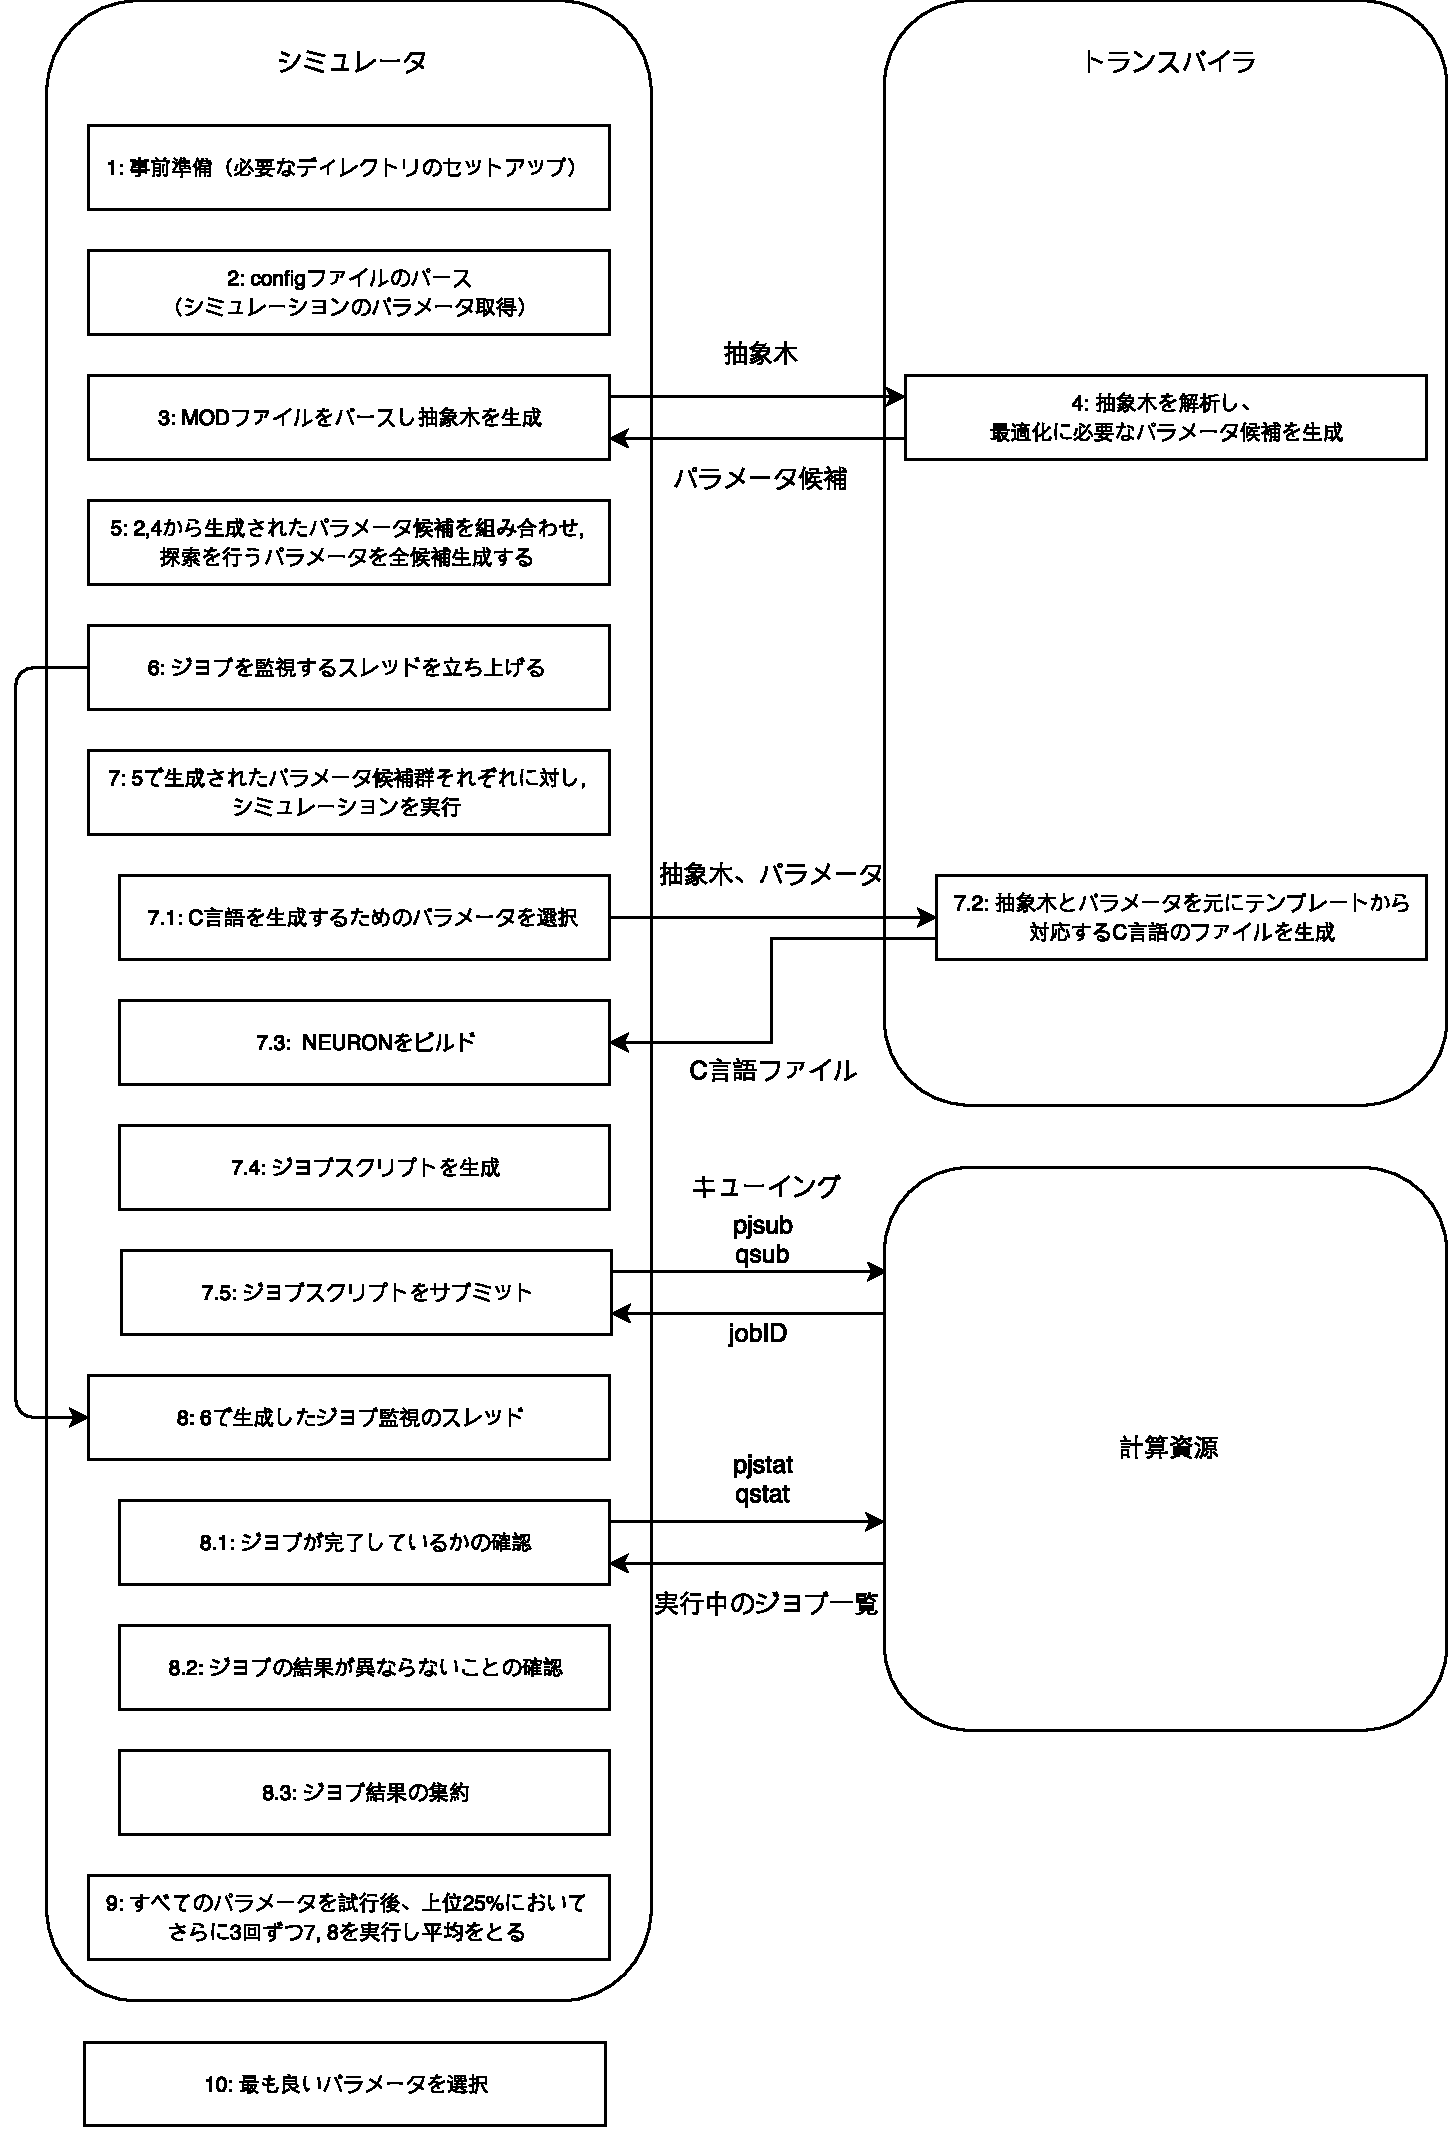
\includegraphics[width=18.0cm]{./images/Genie.pdf}
    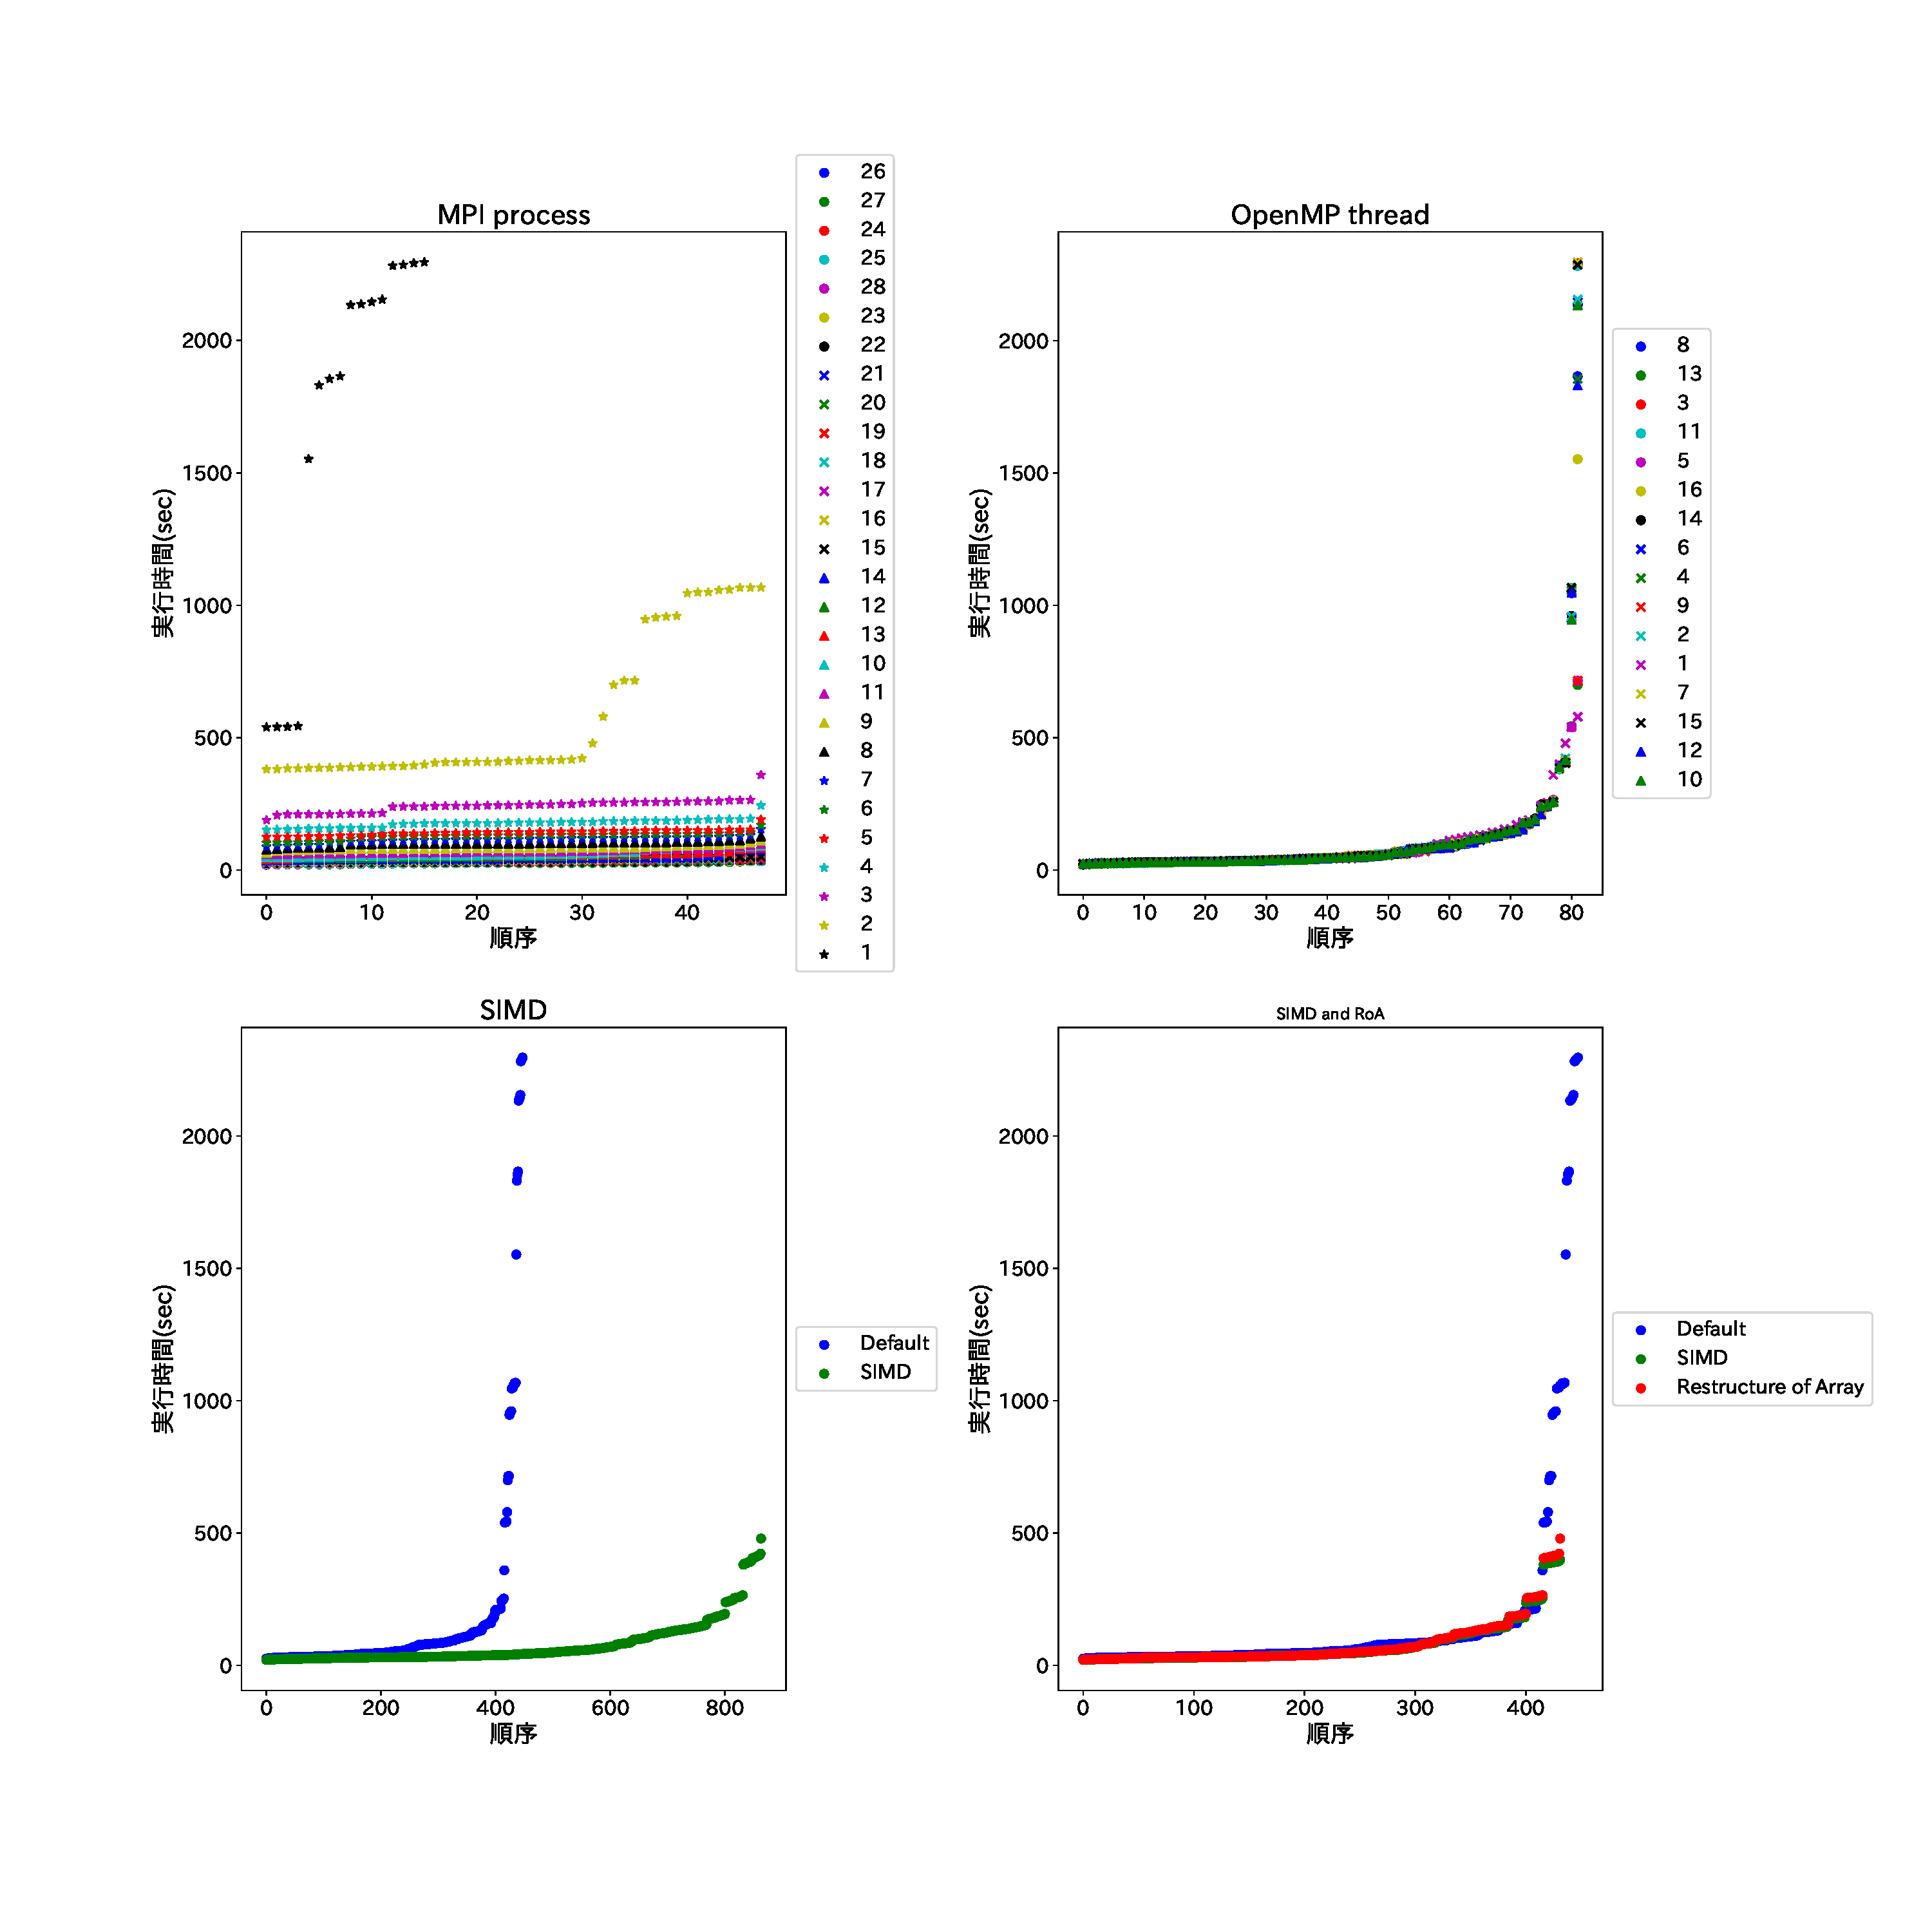
\includegraphics[width=14cm]{./images/cluster-bench.pdf}
    \caption{クラスタ 小規模シミュレーション結果}
    \label{fig:cluster-bench}
 \end{center}
\end{figure}
一方で, この図では実行時間が短い部分が一部の非常に遅い実行時間に影響されて潰れてしまっている.
そこでパラメータと実行時間の関係を見るために, シミュレータでも利用している実行時間の上位25\%を用いる. その結果を図\ref{fig:cluster-bench-top25}に示す.\\
\begin{figure}[htb]
% h:here, t:top, b:bottom, p:page
 \begin{center}
%    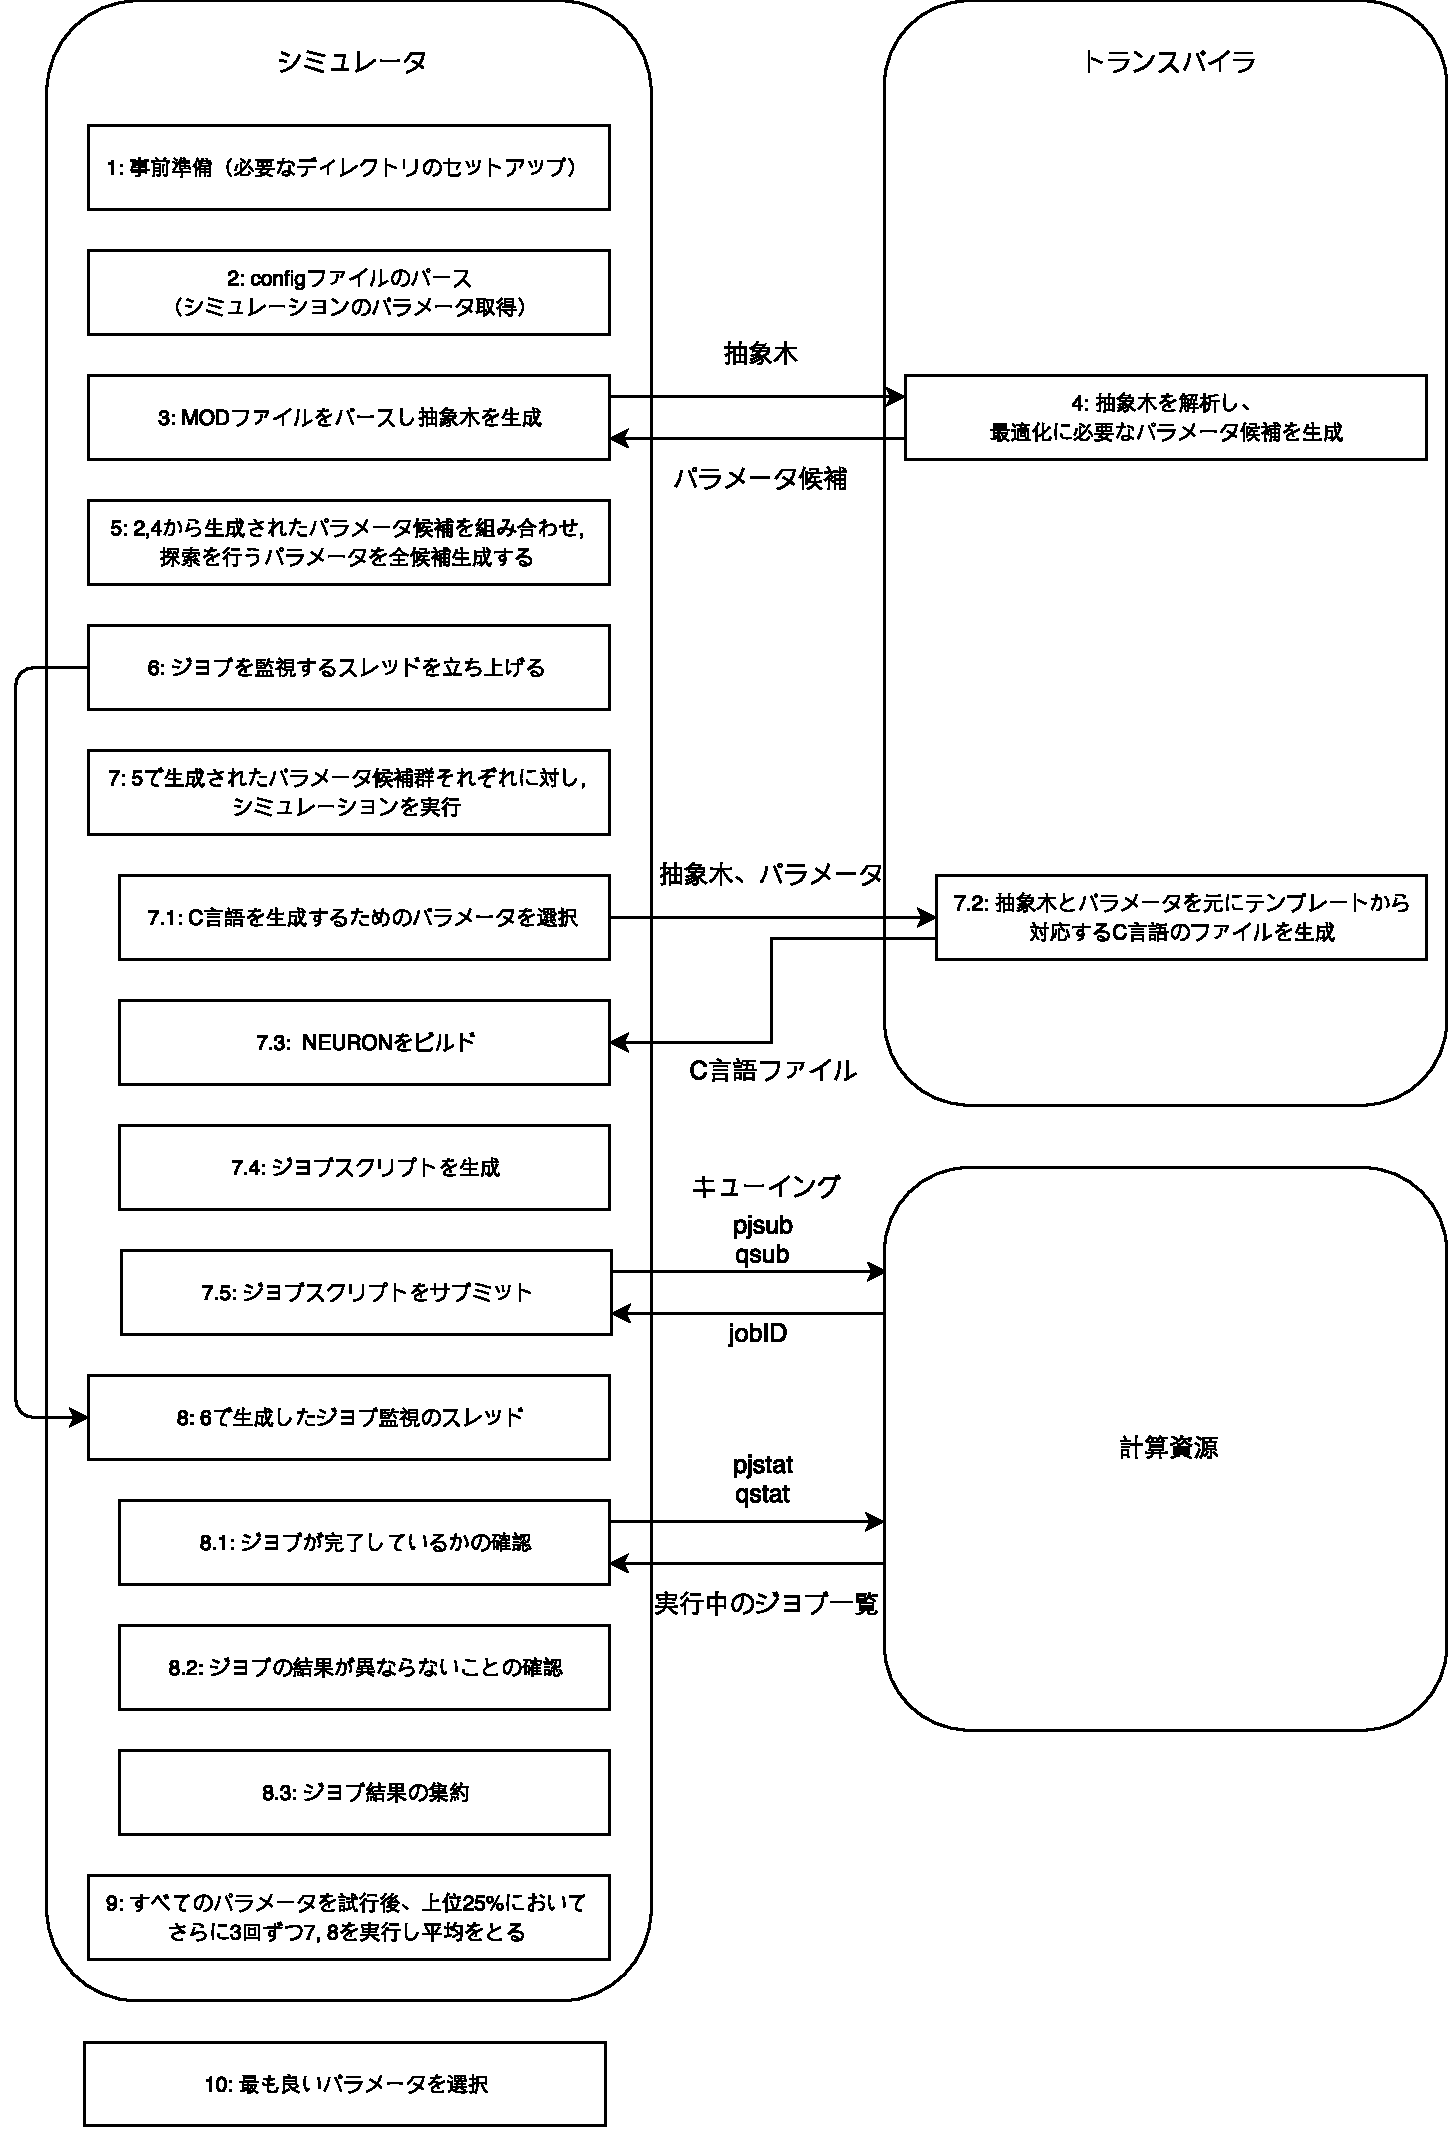
\includegraphics[width=18.0cm]{./images/Genie.pdf}
    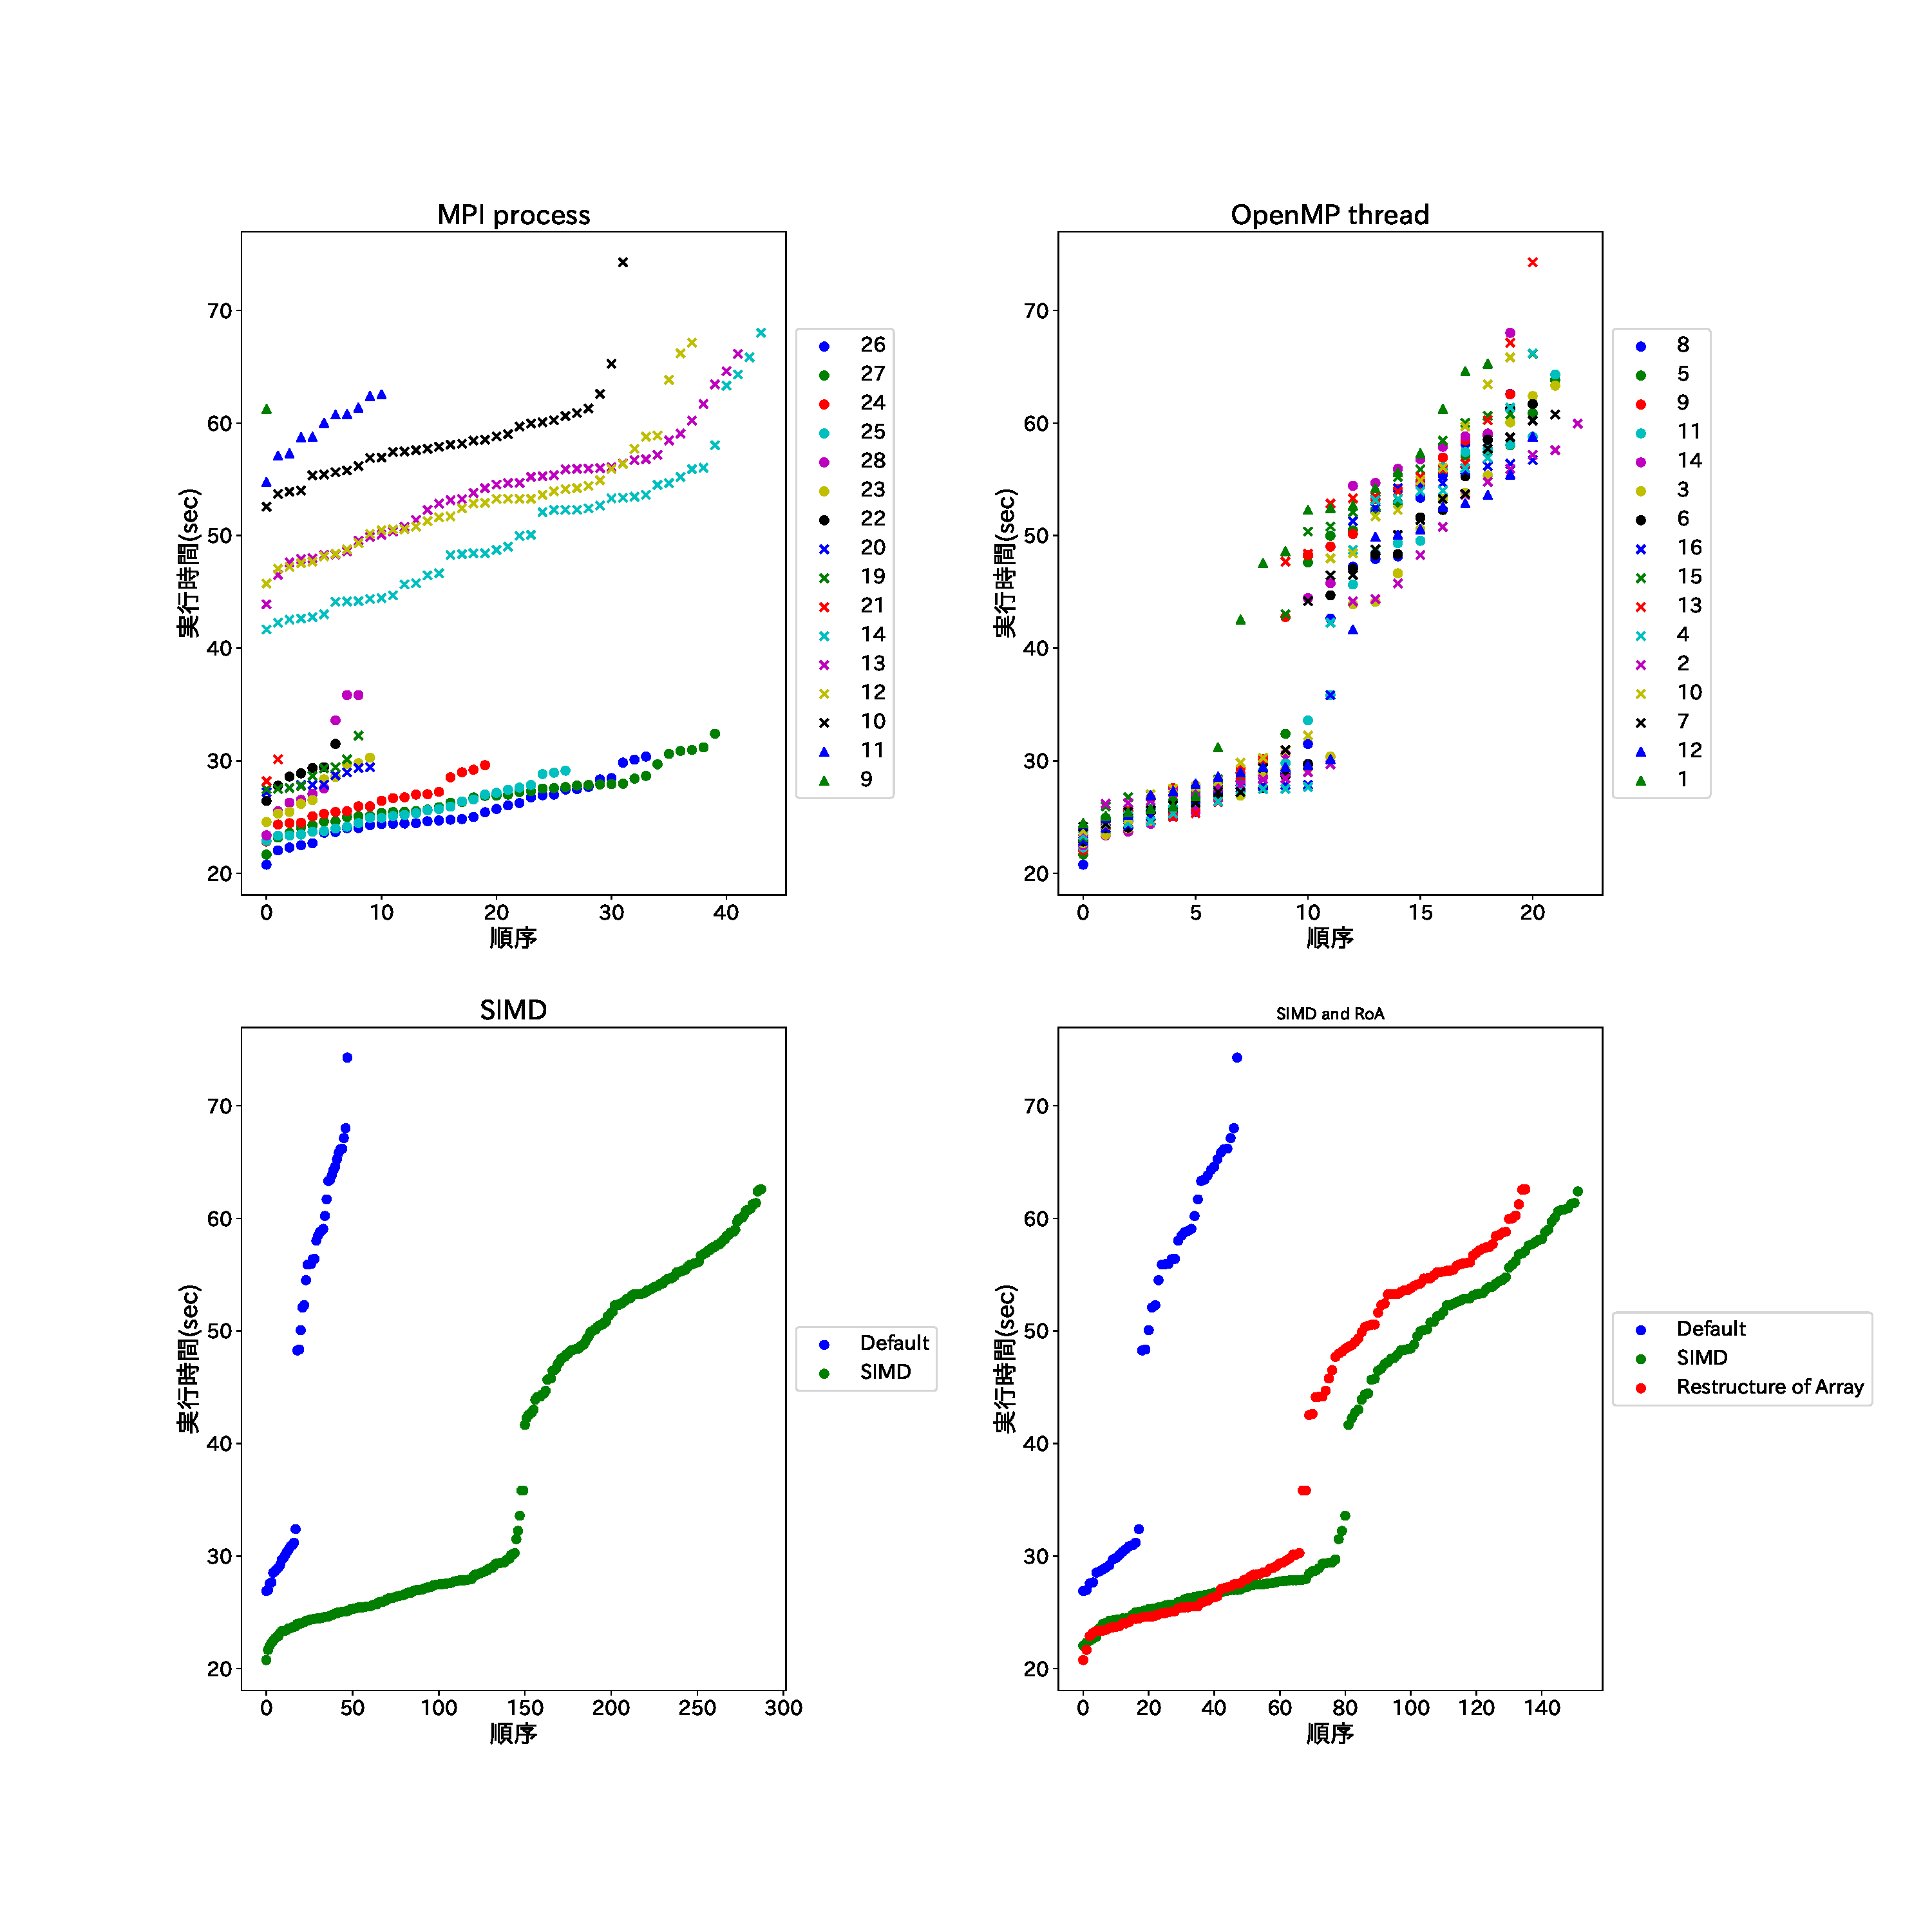
\includegraphics[width=14cm]{./images/cluster-bench-top25.pdf}
    \caption{クラスタ 小規模シミュレーション結果 上位25\%}
    \label{fig:cluster-bench-top25}
 \end{center}
\end{figure}
図\ref{fig:cluster-bench-top25}では, まずMPIプロセス数に関してプロセス数が14以下のものとそれよりも大きいものの間で実行時間に大きな乖離があることがわかる.
本研究において求めるのは, 実行時間がその環境において最も早くなるパラメータ一組であり,
ここで求めたいものは5.2節以降に詳細にシミュレーションを行う意義のあるパラメータ候補であるため,
ためこのように明確に乖離が見られるパラメータは探索対象から除外することができる.\\
同様にして, 他の条件を固定した状態でパラメータの除外を行いパラメータによる有意差が生まれなくなるまで絞り込みを行った結果が図\ref{fig:cluster-bench-adjusted-final}である.\\
\begin{figure}[htb]
% h:here, t:top, b:bottom, p:page
\begin{center}
%    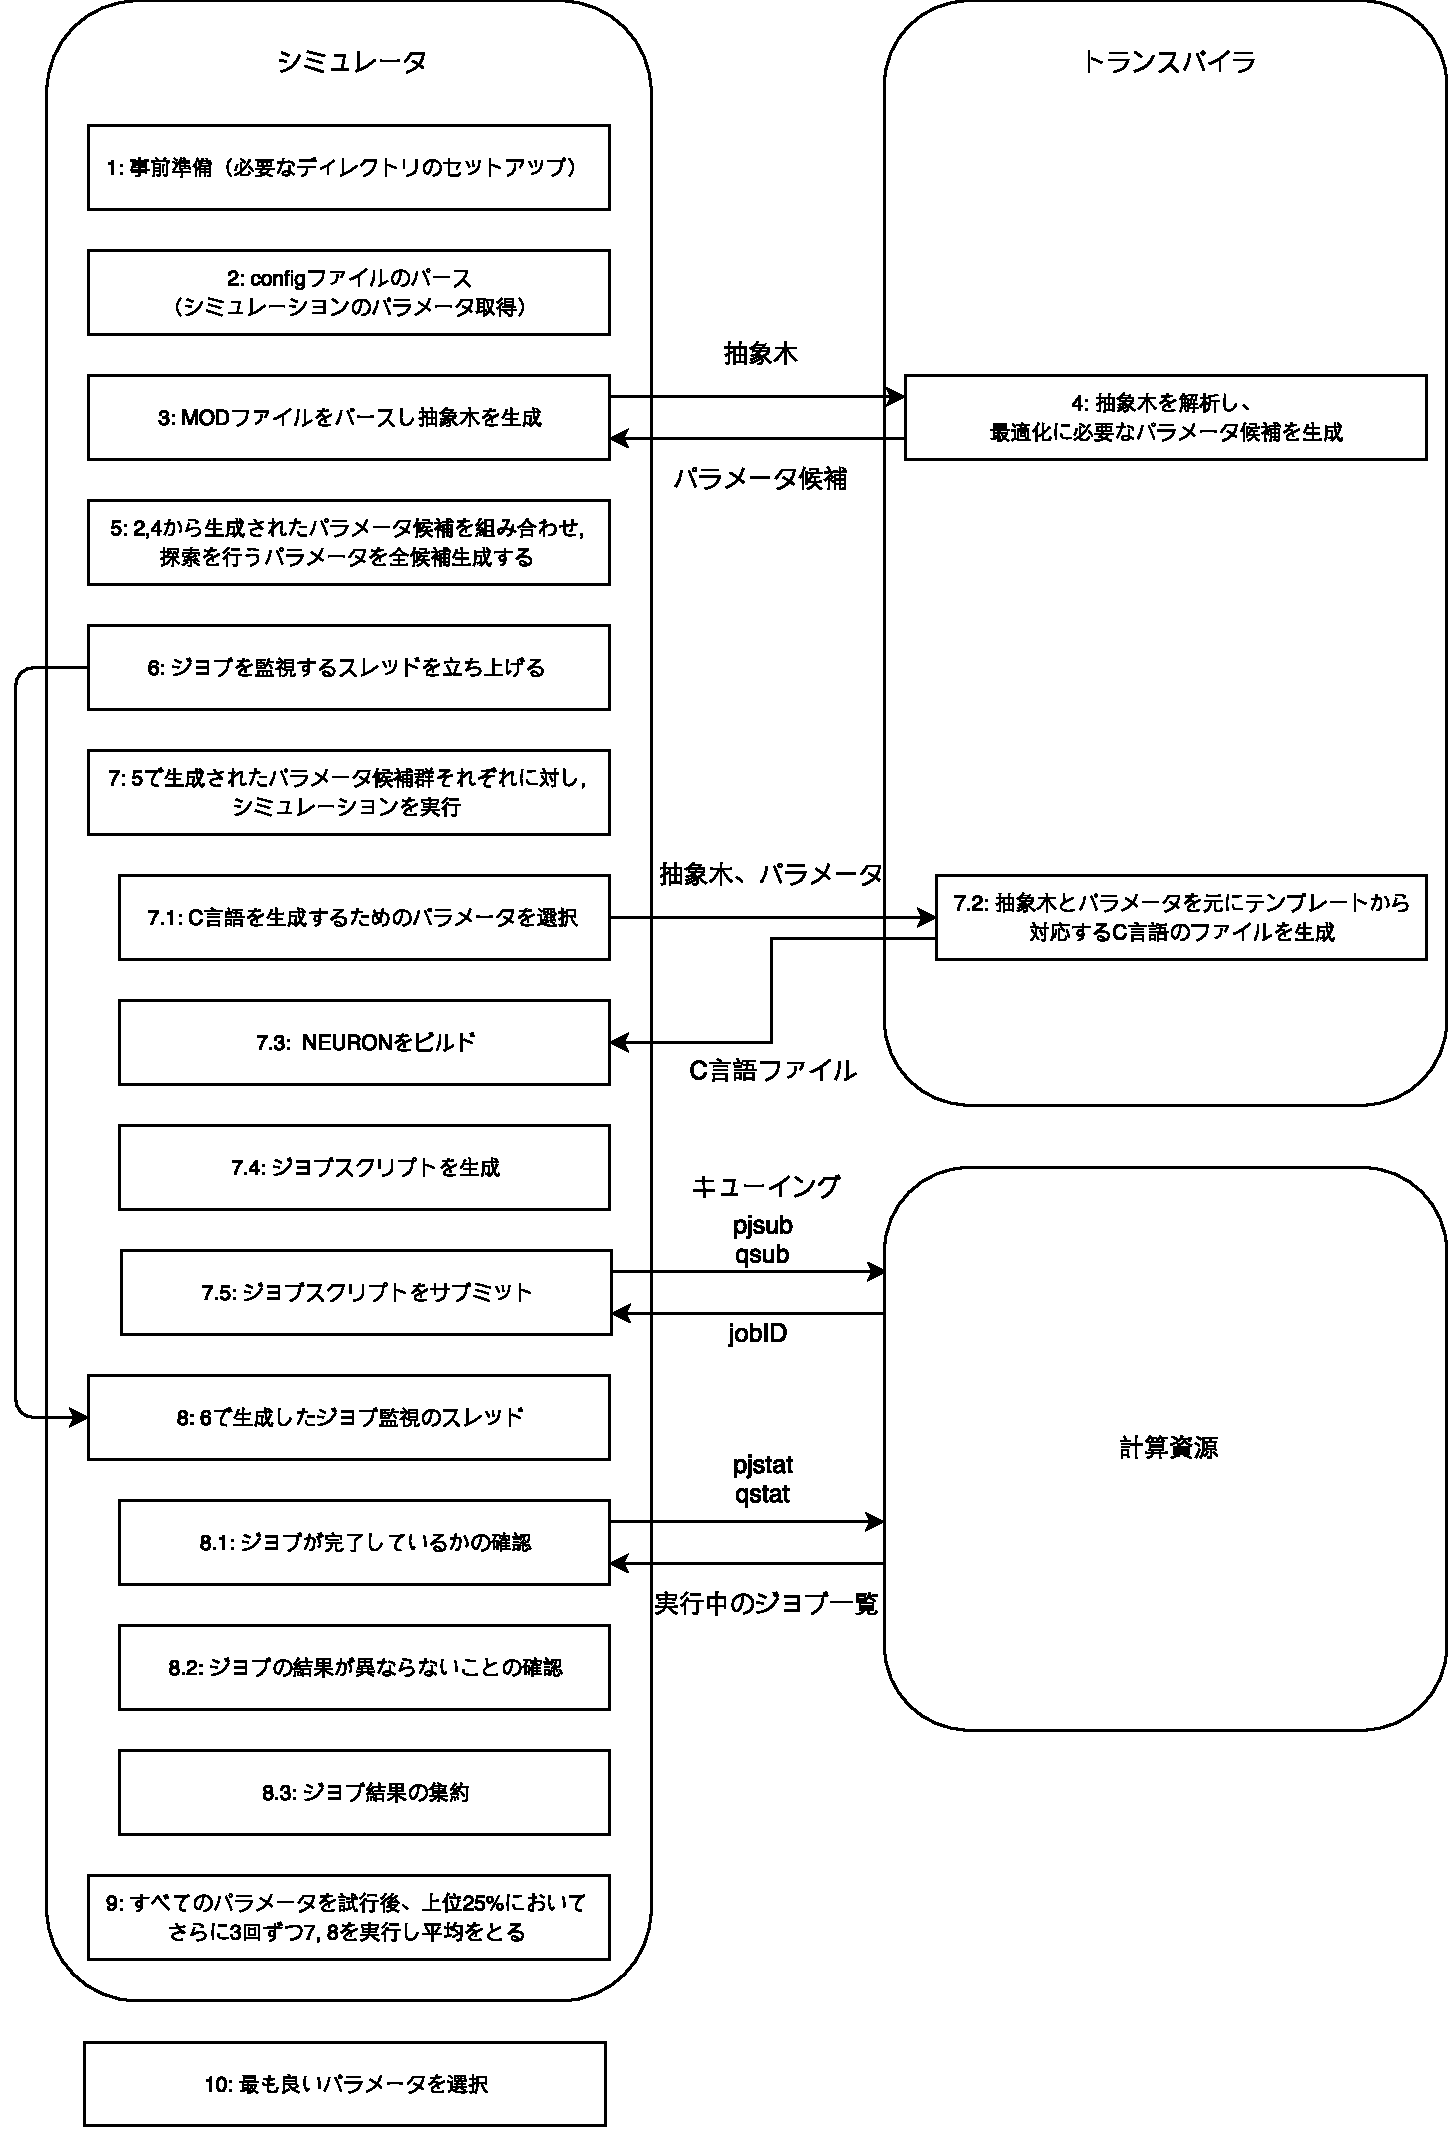
\includegraphics[width=18.0cm]{./images/Genie.pdf}
    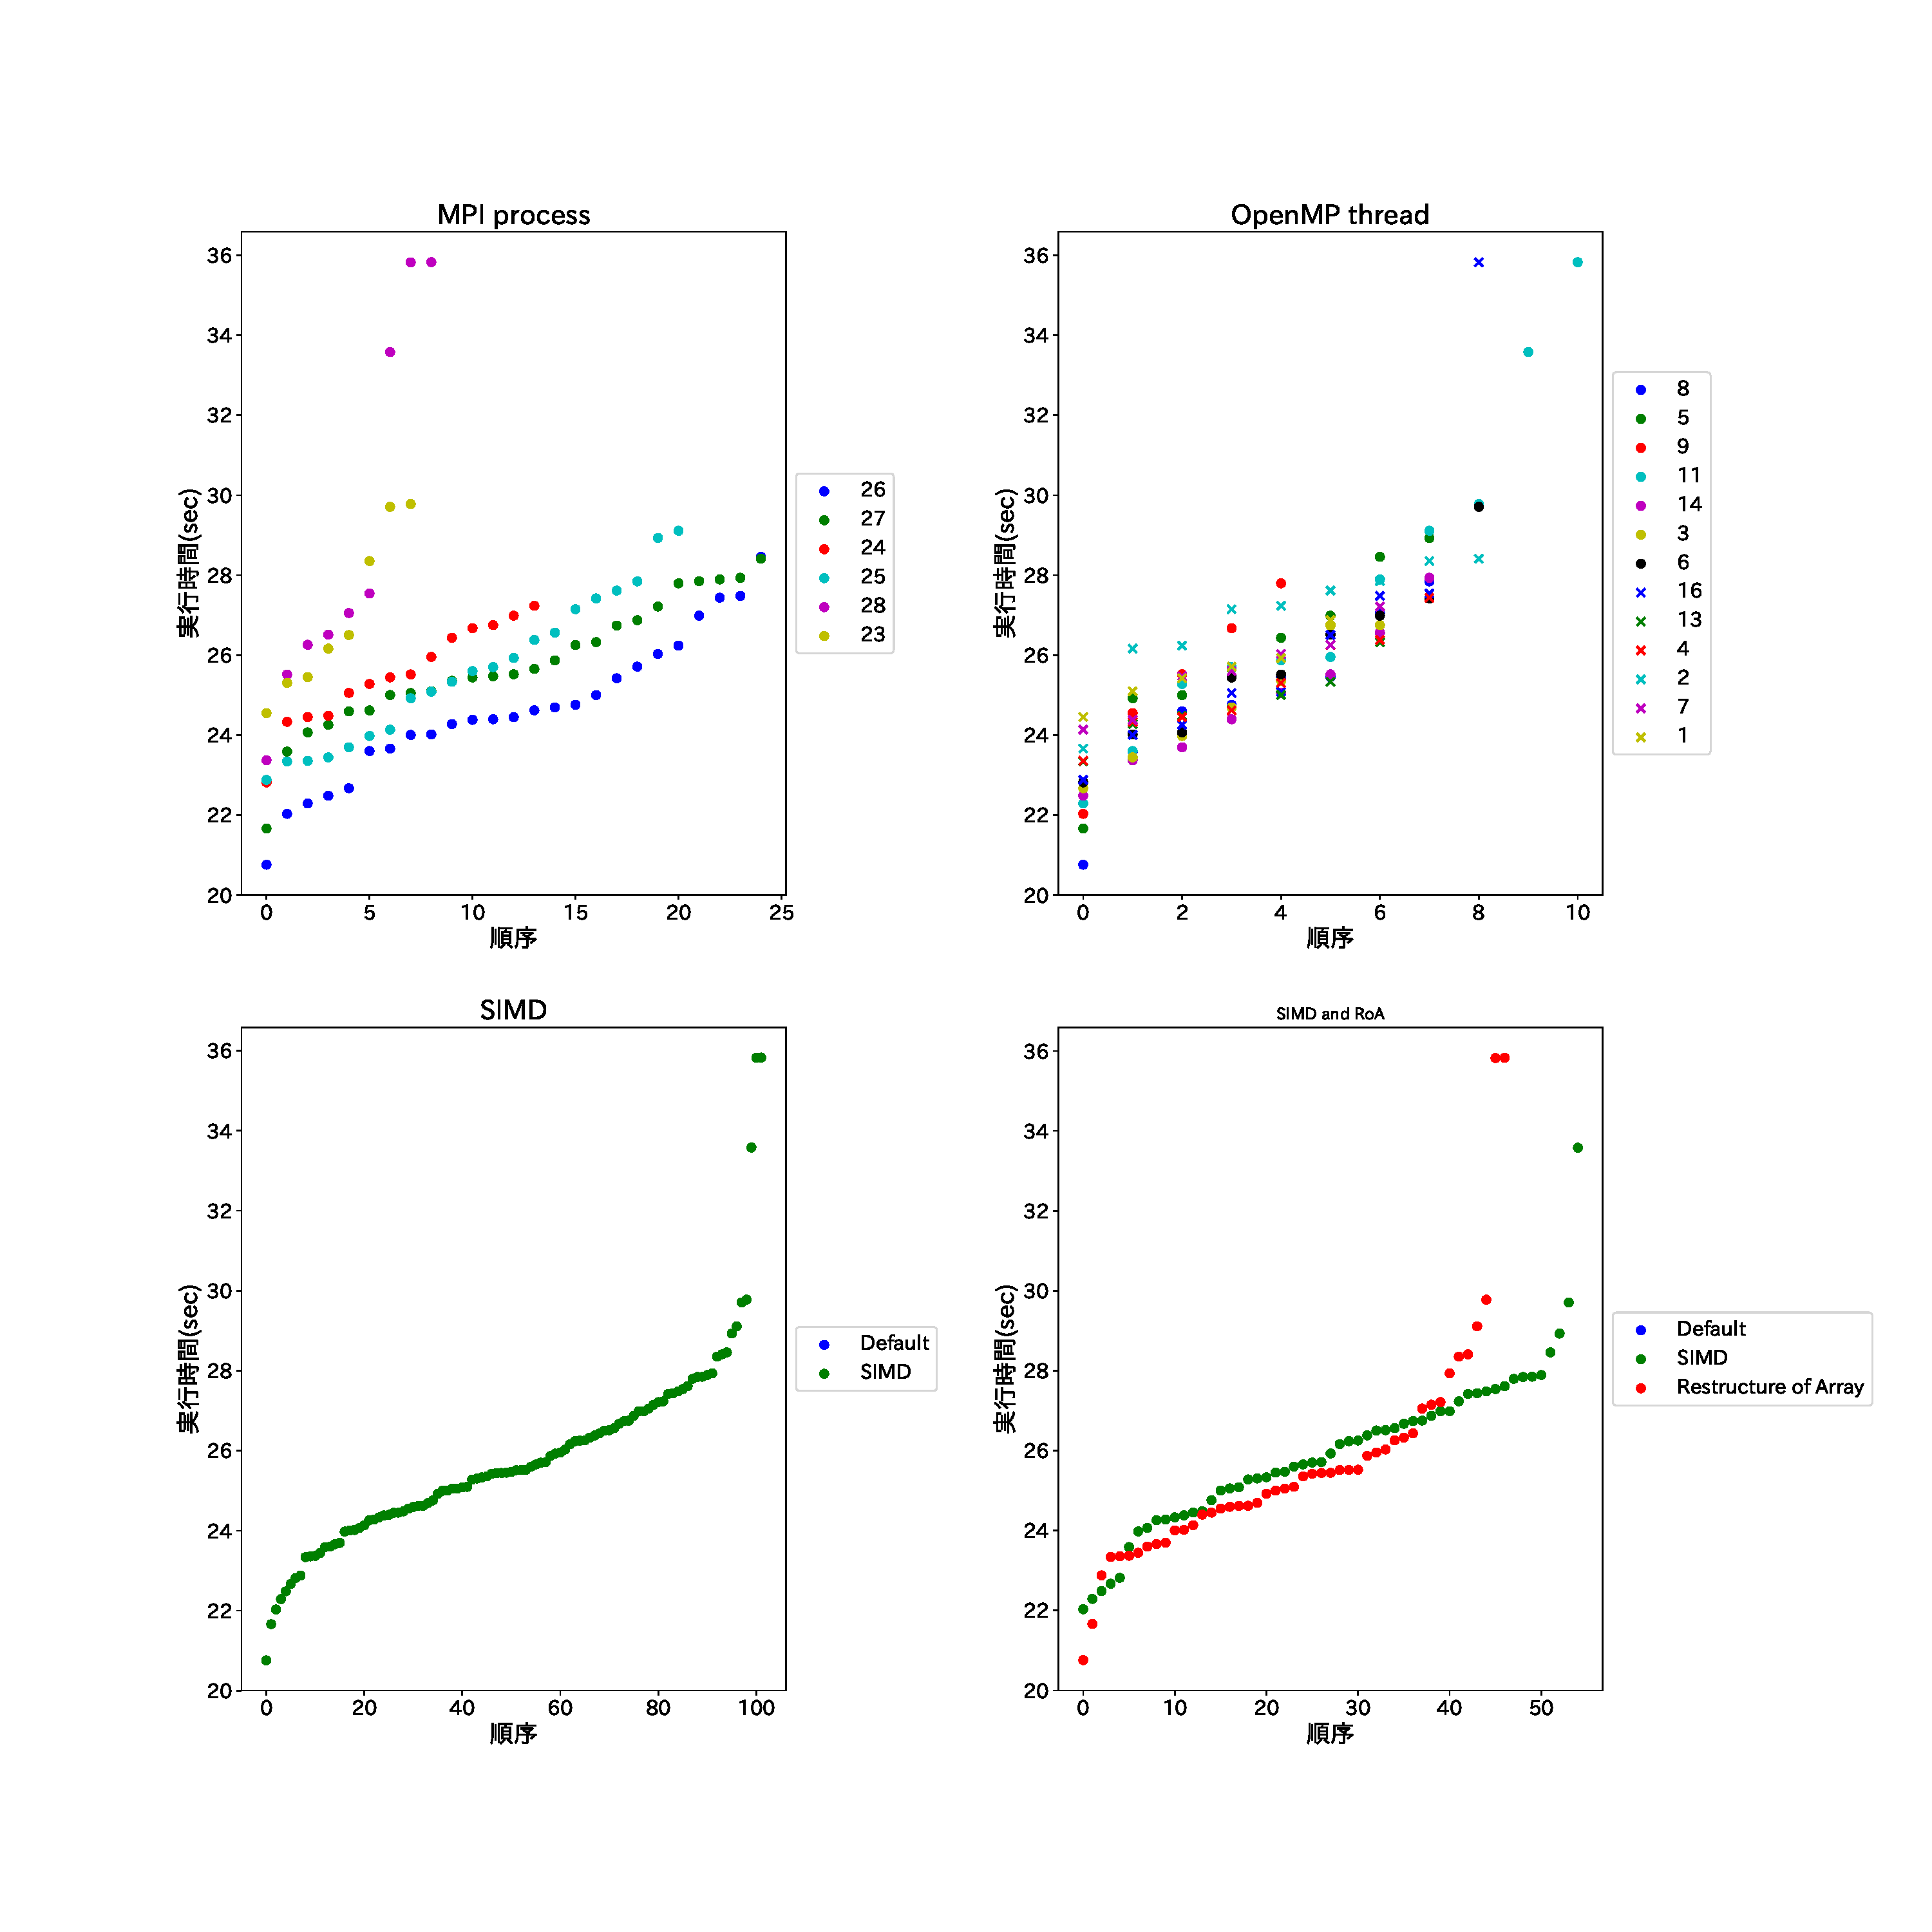
\includegraphics[width=14cm]{./images/cluster-bench-adjusted-final.pdf}
    \caption{クラスタ 小規模シミュレーション結果 パラメータ絞り込み後}
    \label{fig:cluster-bench-adjusted-final}
\end{center}
\end{figure}
\clearpage
また絞り込みを行った後のパラメータは次のようになる.\\
\begin{table}[htb]
  \caption {クラスタでの絞り込み後のパラメータ}
  \begin{center}
    \begin{tabular}{|c|p{12cm}|}
      \hline
      パラメータ & 値の範囲\\ \hline
      ノード数 & 1\\ \hline
      MPIプロセス数 & 23〜28\\ \hline
      OpenMPスレッド数 & [1, 2, 3, 4, 5, 6, 7, 8, 9, 11, 13, 14, 16]\\ \hline
      SIMD化 & 行う\\ \hline
      配列のくくり出し & 行う or 行わない\\ \hline
    \end{tabular}
  \end{center}
\end{table}

\subsubsection{京環境}
\begin{table}[htb]
  \caption {京でのパラメータ}
  \begin{center}
    \begin{tabular}{|c|p{12cm}|}
      \hline
      パラメータ & 値の範囲\\ \hline
      ノード数 & 8\\ \hline
      MPIプロセス数 & 1〜8\\ \hline
      OpenMPスレッド数 & 1〜16\\ \hline
      SIMD化 & 行う or 行わない\\ \hline
      配列のくくり出し & 行う(SIMD化を行っているならば) or 行わない\\ \hline
      シミュレーション時間 & 100ms\\ \hline
      神経細胞数 & 256\\ \hline
    \end{tabular}
  \end{center}
\end{table}
京においてもクラスタ同様パラメータの絞り込みを小規模シミュレーションを用いて行った.\\
図\ref{fig:k-bench}のMPIプロセス数に着目すると, それぞれのプロセス数に対し30番目前後で大きな
隔たりがあることがわかる. SIMDのグラフにおいてもSIMDがデフォルトのソースコードを大きく上回っていること,
またシミュレーションの設定上SIMDとそうでないものが2対1の比率であり,
30番目付近を境としたMPIプロセス数における比率と同じであることからこの隔たりはSIMD化が影響していることがわかる.\\
\begin{figure}[htb]
% h:here, t:top, b:bottom, p:page
\begin{center}
%    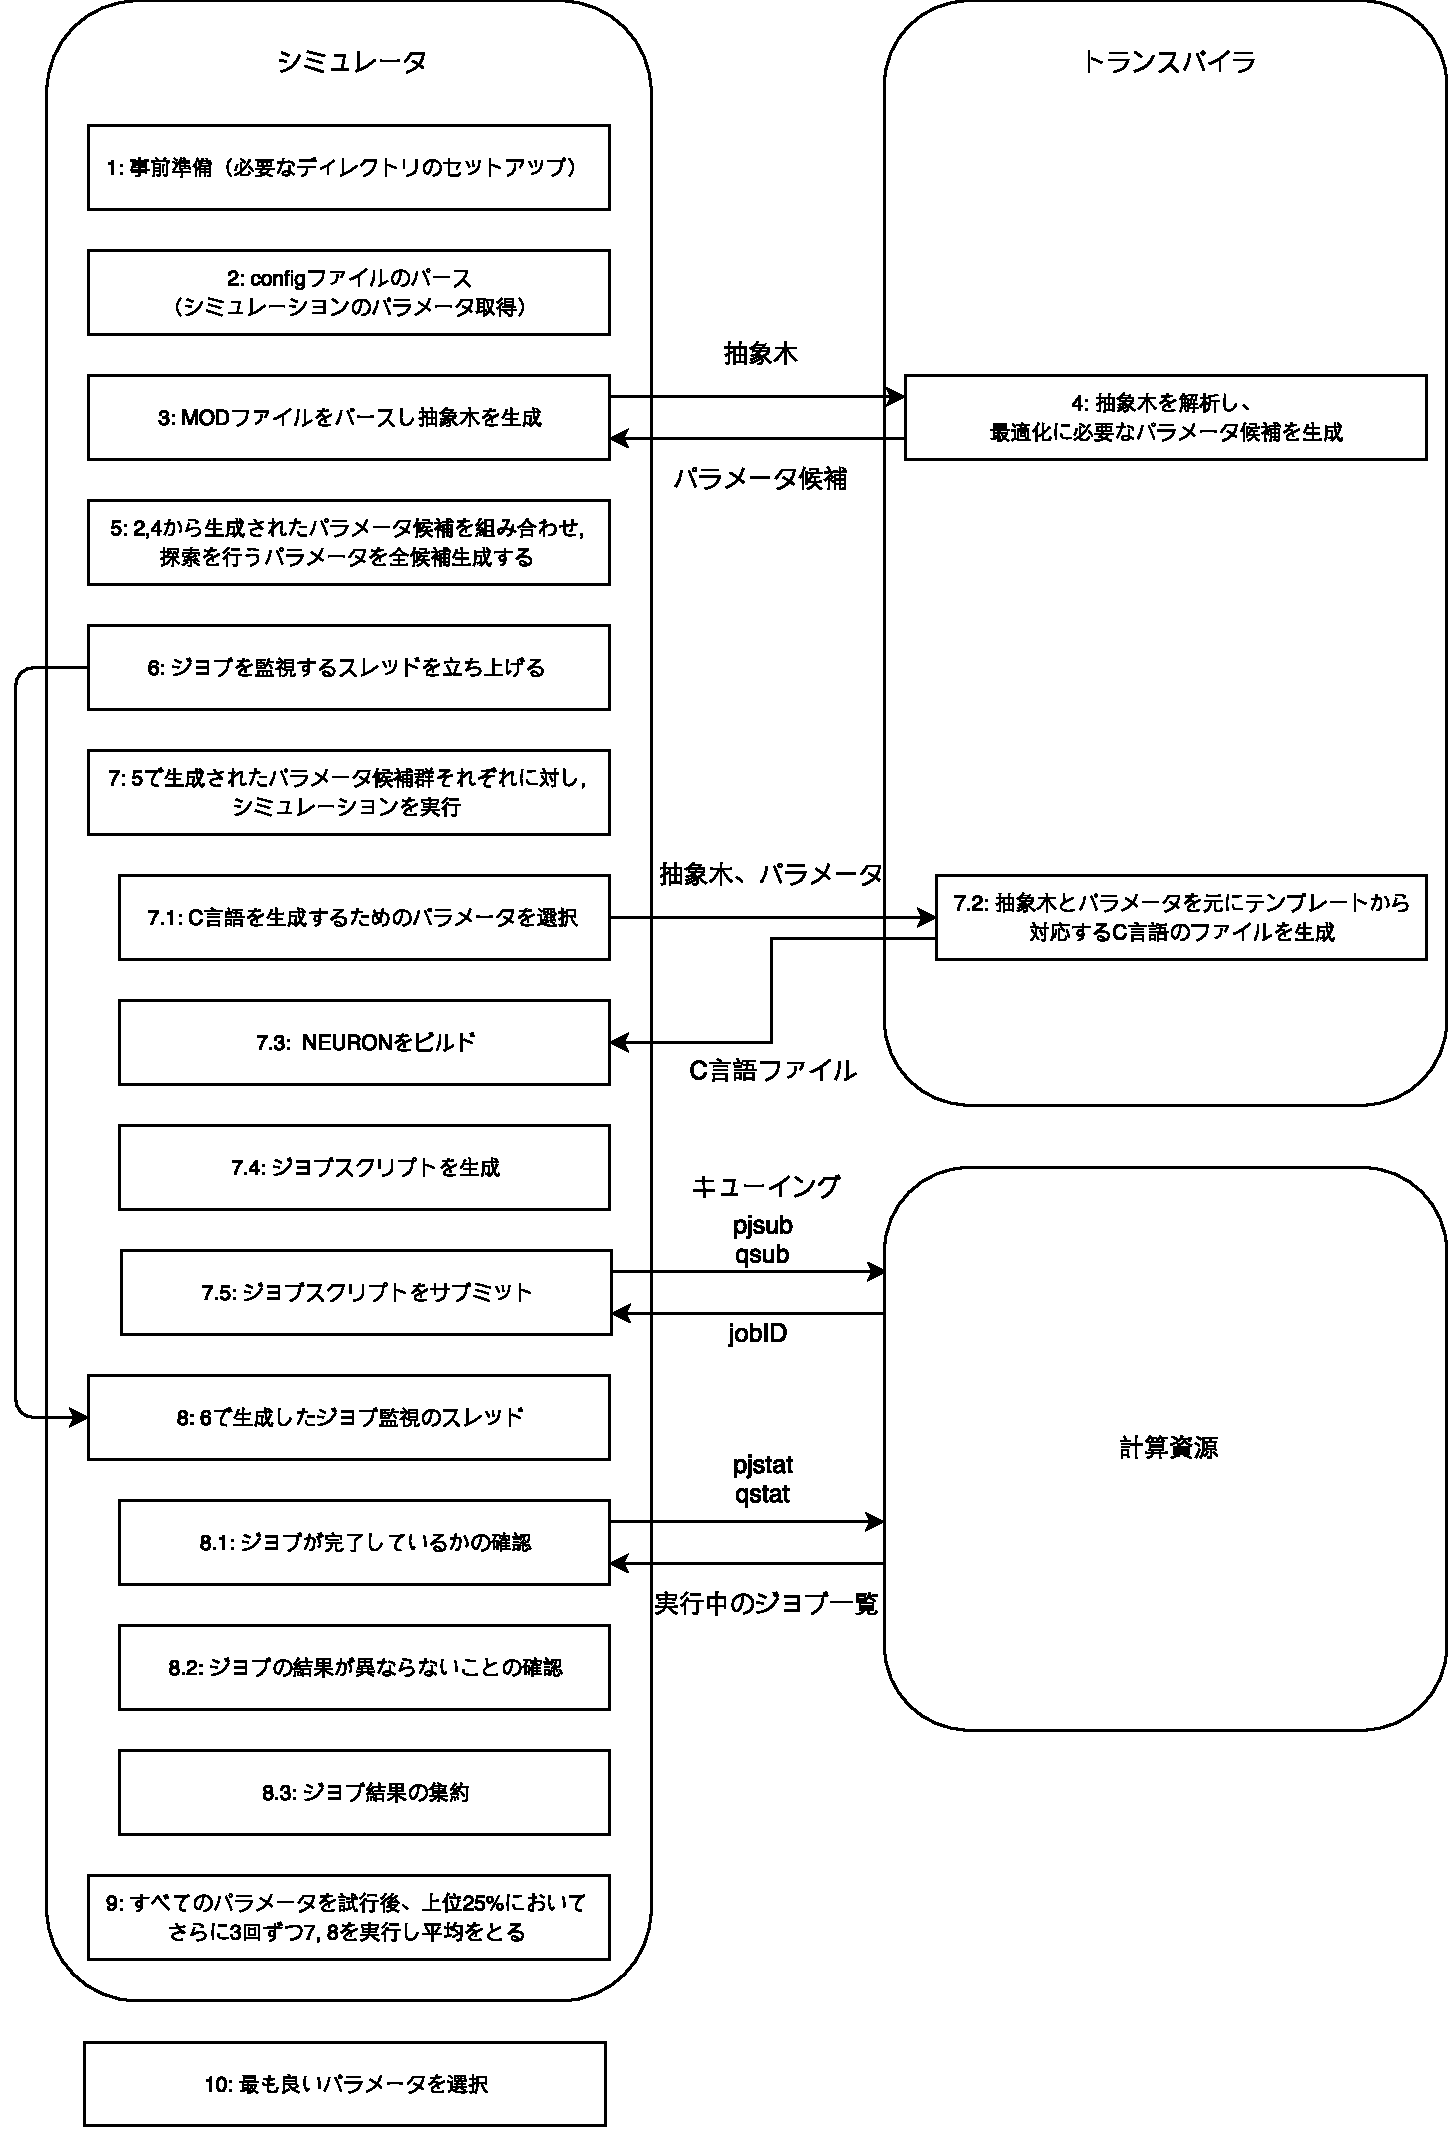
\includegraphics[width=18.0cm]{./images/Genie.pdf}
    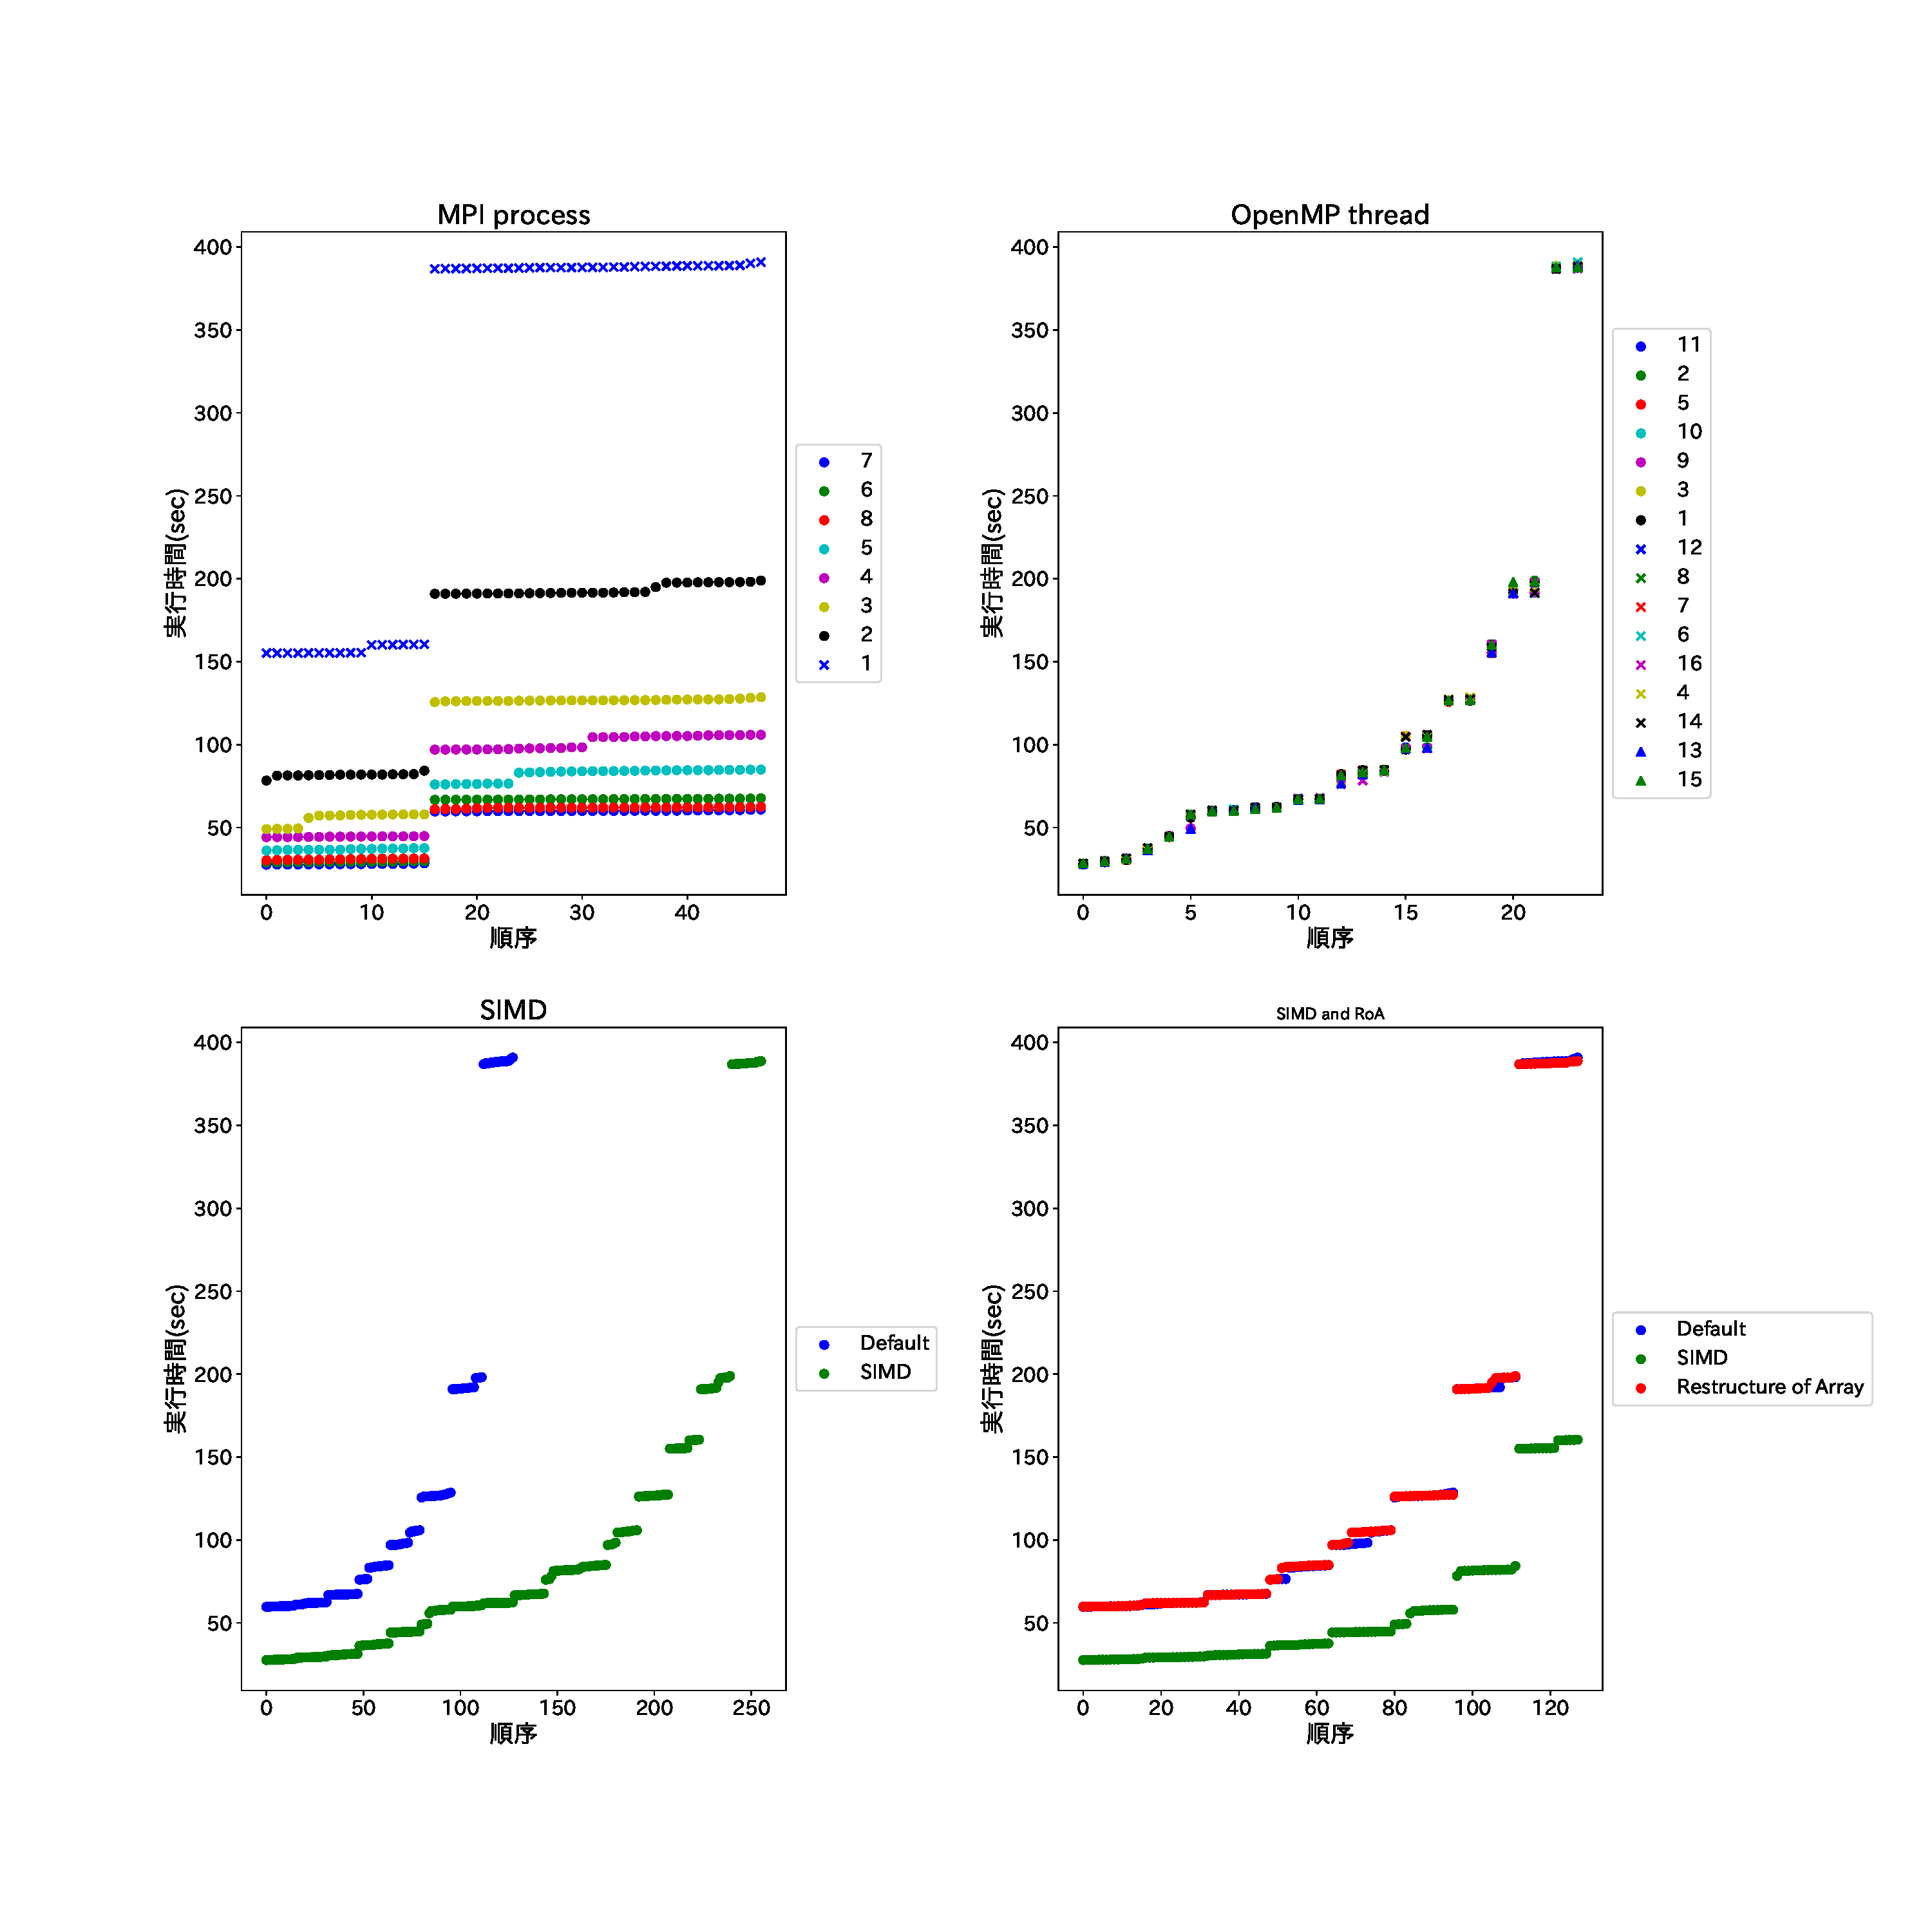
\includegraphics[width=14cm]{./images/k-bench.pdf}
    \caption{京 小規模シミュレーション結果}
    \label{fig:k-bench}
\end{center}
\end{figure}
\clearpage
一方で, シミュレーション結果の実行時間が早い上位25\%のパラメータを示した図\ref{fig:k-bench-top25}では,
プロセス数8のものが他のプロセス数と比較して抜きん出て高速であることが読み取れる.
また, SIMD化されていないパラメータ候補はすでに除外されており,
候補数がすでに十分制限されているためプロセス数とSIMD化のみを絞り込みの条件として用いた.\\

\begin{figure}[htb]
% h:here, t:top, b:bottom, p:page
\begin{center}
%    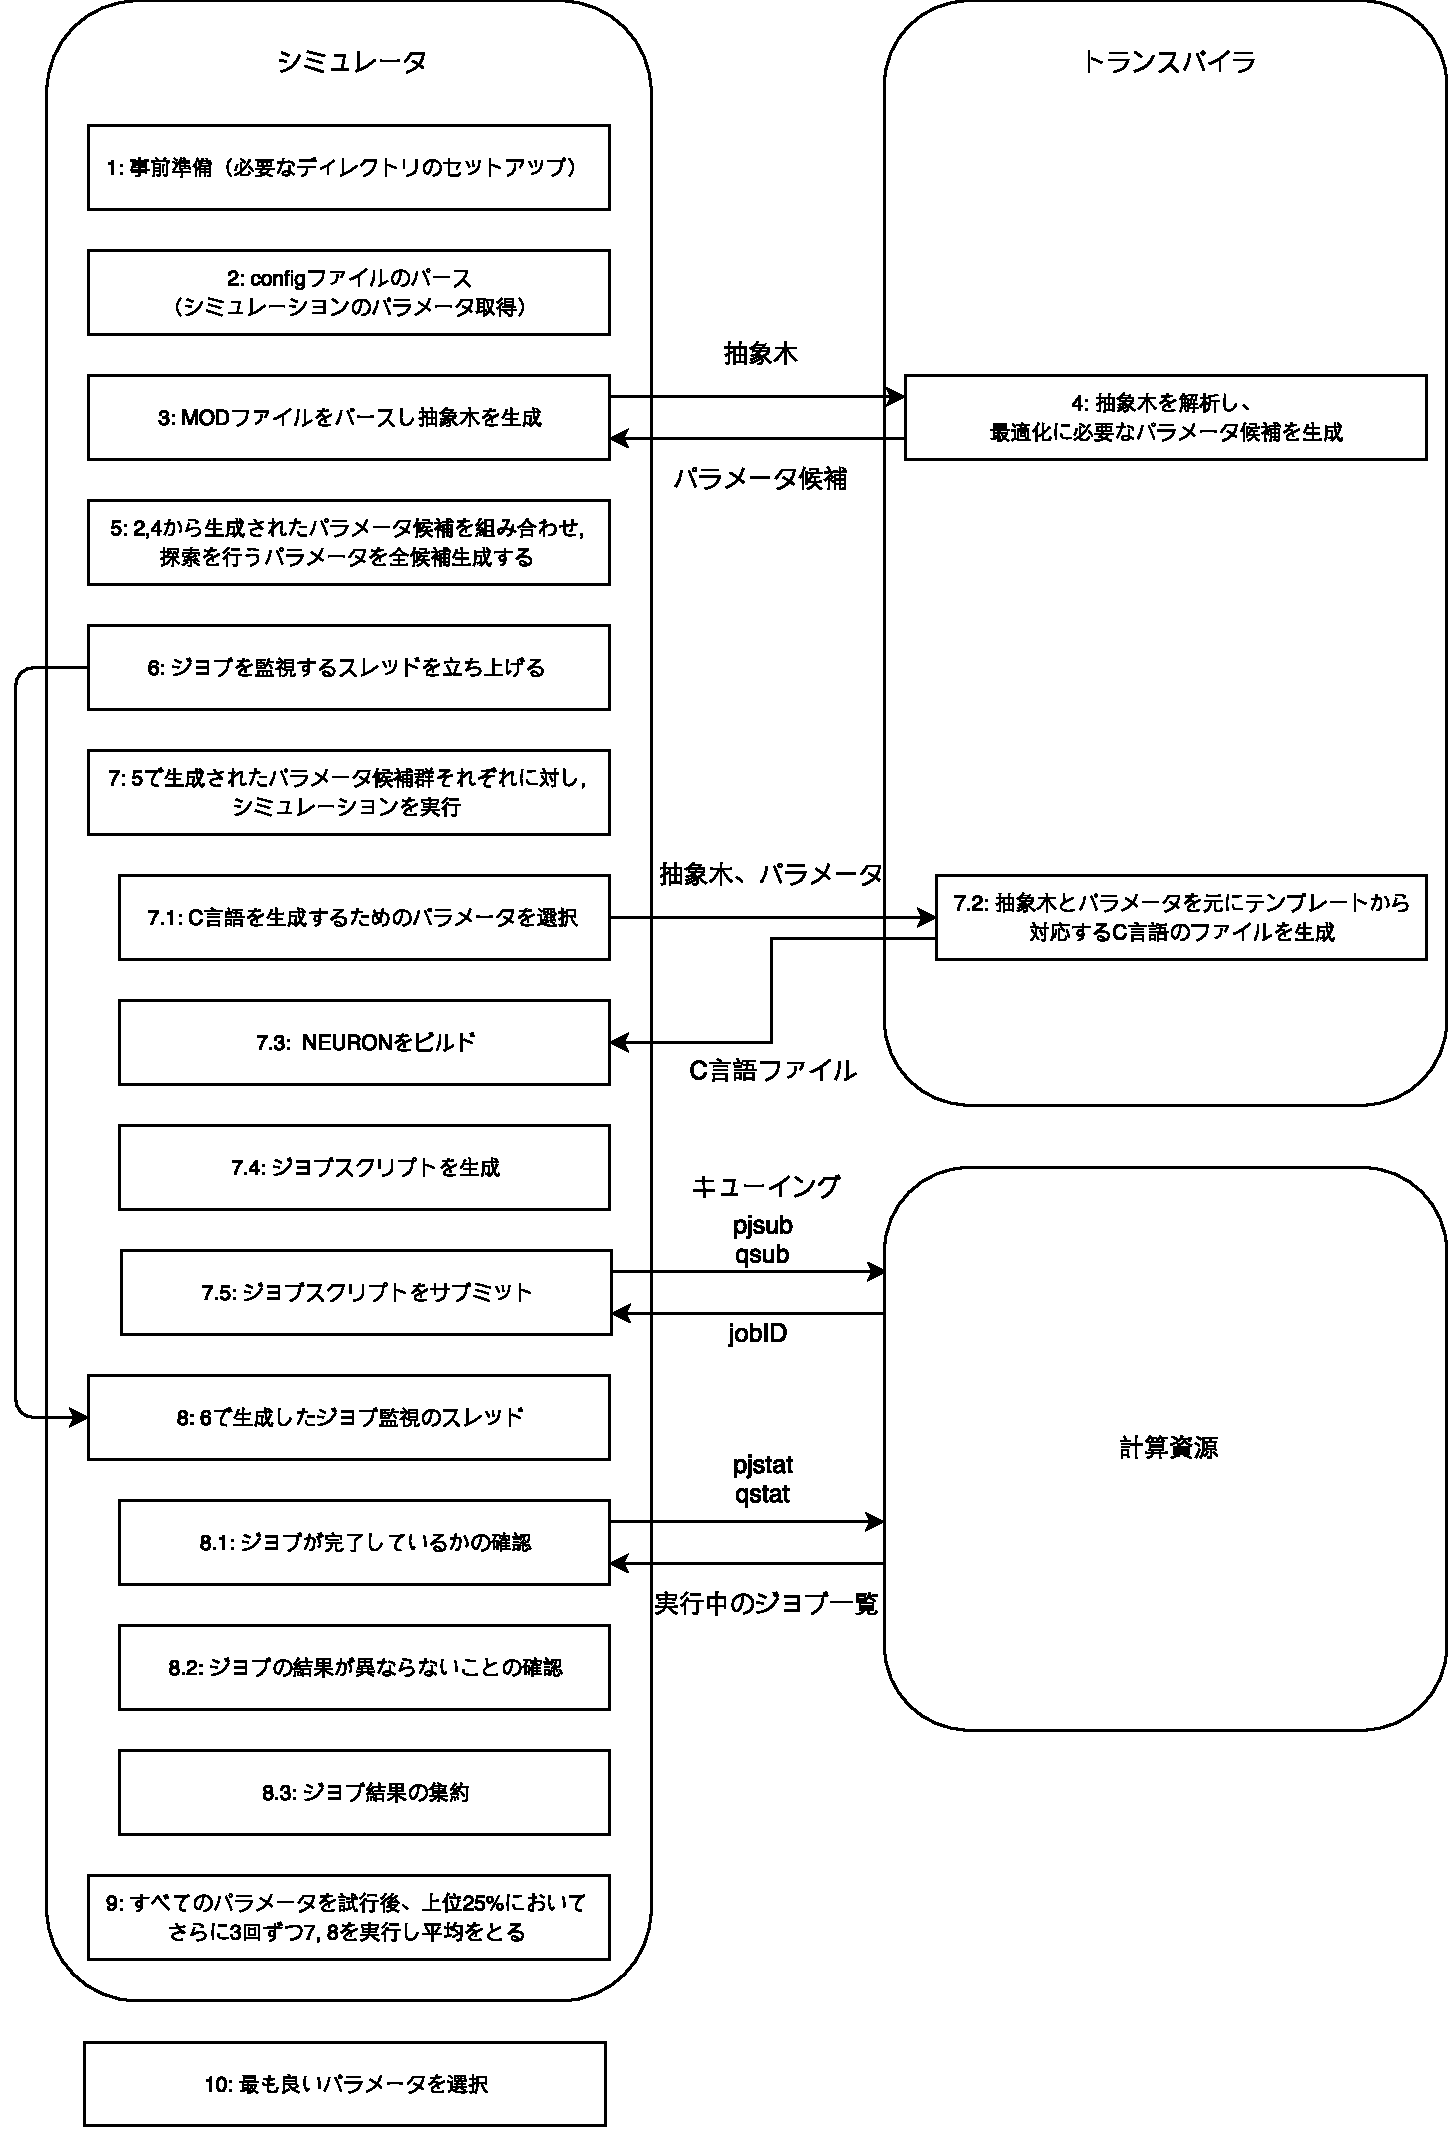
\includegraphics[width=18.0cm]{./images/Genie.pdf}
    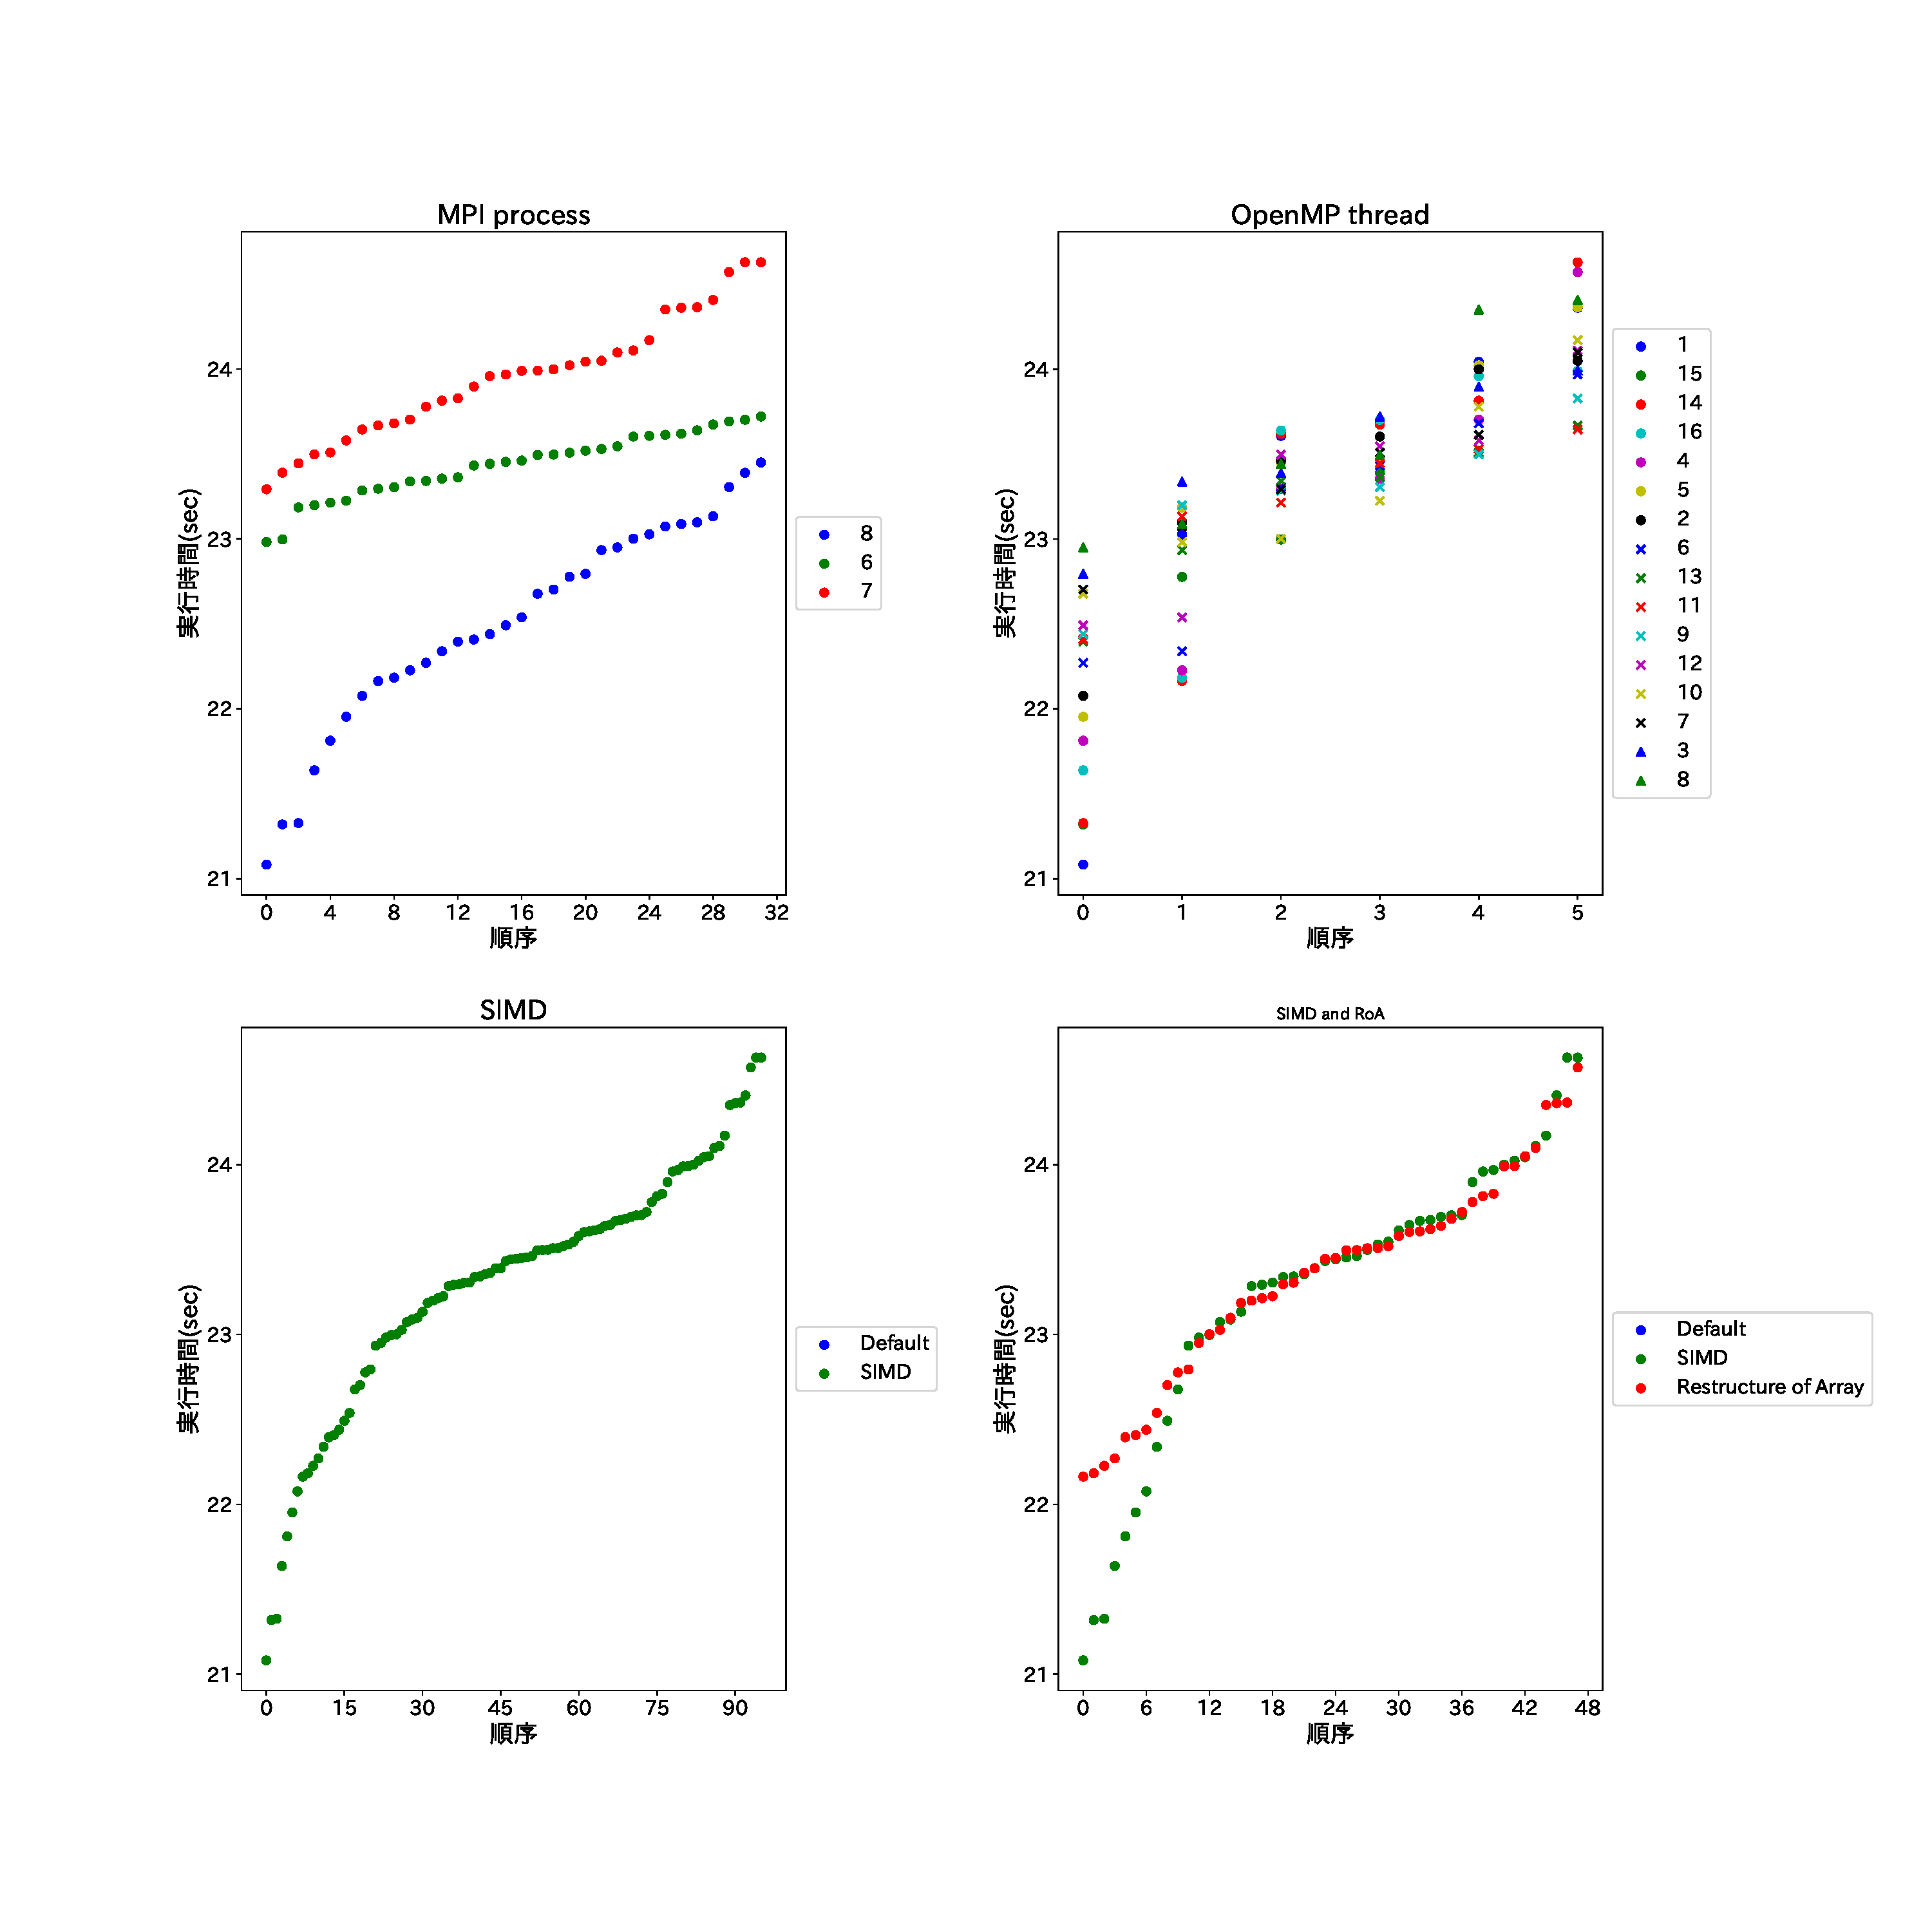
\includegraphics[width=14cm]{./images/k-bench-top25.pdf}
    \caption{京 小規模シミュレーション結果 top25\%}
    \label{fig:k-bench-top25}
\end{center}
\end{figure}

以下がクラスタと同様に京で小規模シミュレーションを元に絞り込みを行ったパラメータ候補である.\\
クラスタと京の絞り込み後のパラメータから( TODO: mpi openmp)で述べたように,
小規模環境においてはMPIプロセスが最適化の中で大きな役割を果たすことがわかり,
コアのほとんどをMPIプロセスで利用する場合に高速になる傾向が強いことがわかった.\\
また京において, 配列のくくり出しをしない方がより高速化されていることが図\ref{fig:k-bench-adjusted-final}の右下のグラフから読み取れるが,
これは京がアーキテクチャとしてSIMDに強く京で用いられるコンパイラもSIMDに適していることが原因であると推察される.
\begin{table}[htb]
  \caption {京でのパラメータ 絞り込み後}
  \begin{center}
    \begin{tabular}{|c|p{12cm}|}
      \hline
      パラメータ & 値の範囲\\ \hline
      ノード数 & 8\\ \hline
      MPIプロセス数 & 8\\ \hline
      OpenMPスレッド数 & 1〜16\\ \hline
      SIMD化 & 行う\\ \hline
      配列のくくり出し & 行う(SIMD化を行っているならば) or 行わない\\ \hline
    \end{tabular}
  \end{center}
\end{table}

\begin{figure}[htb]
% h:here, t:top, b:bottom, p:page
\begin{center}
%    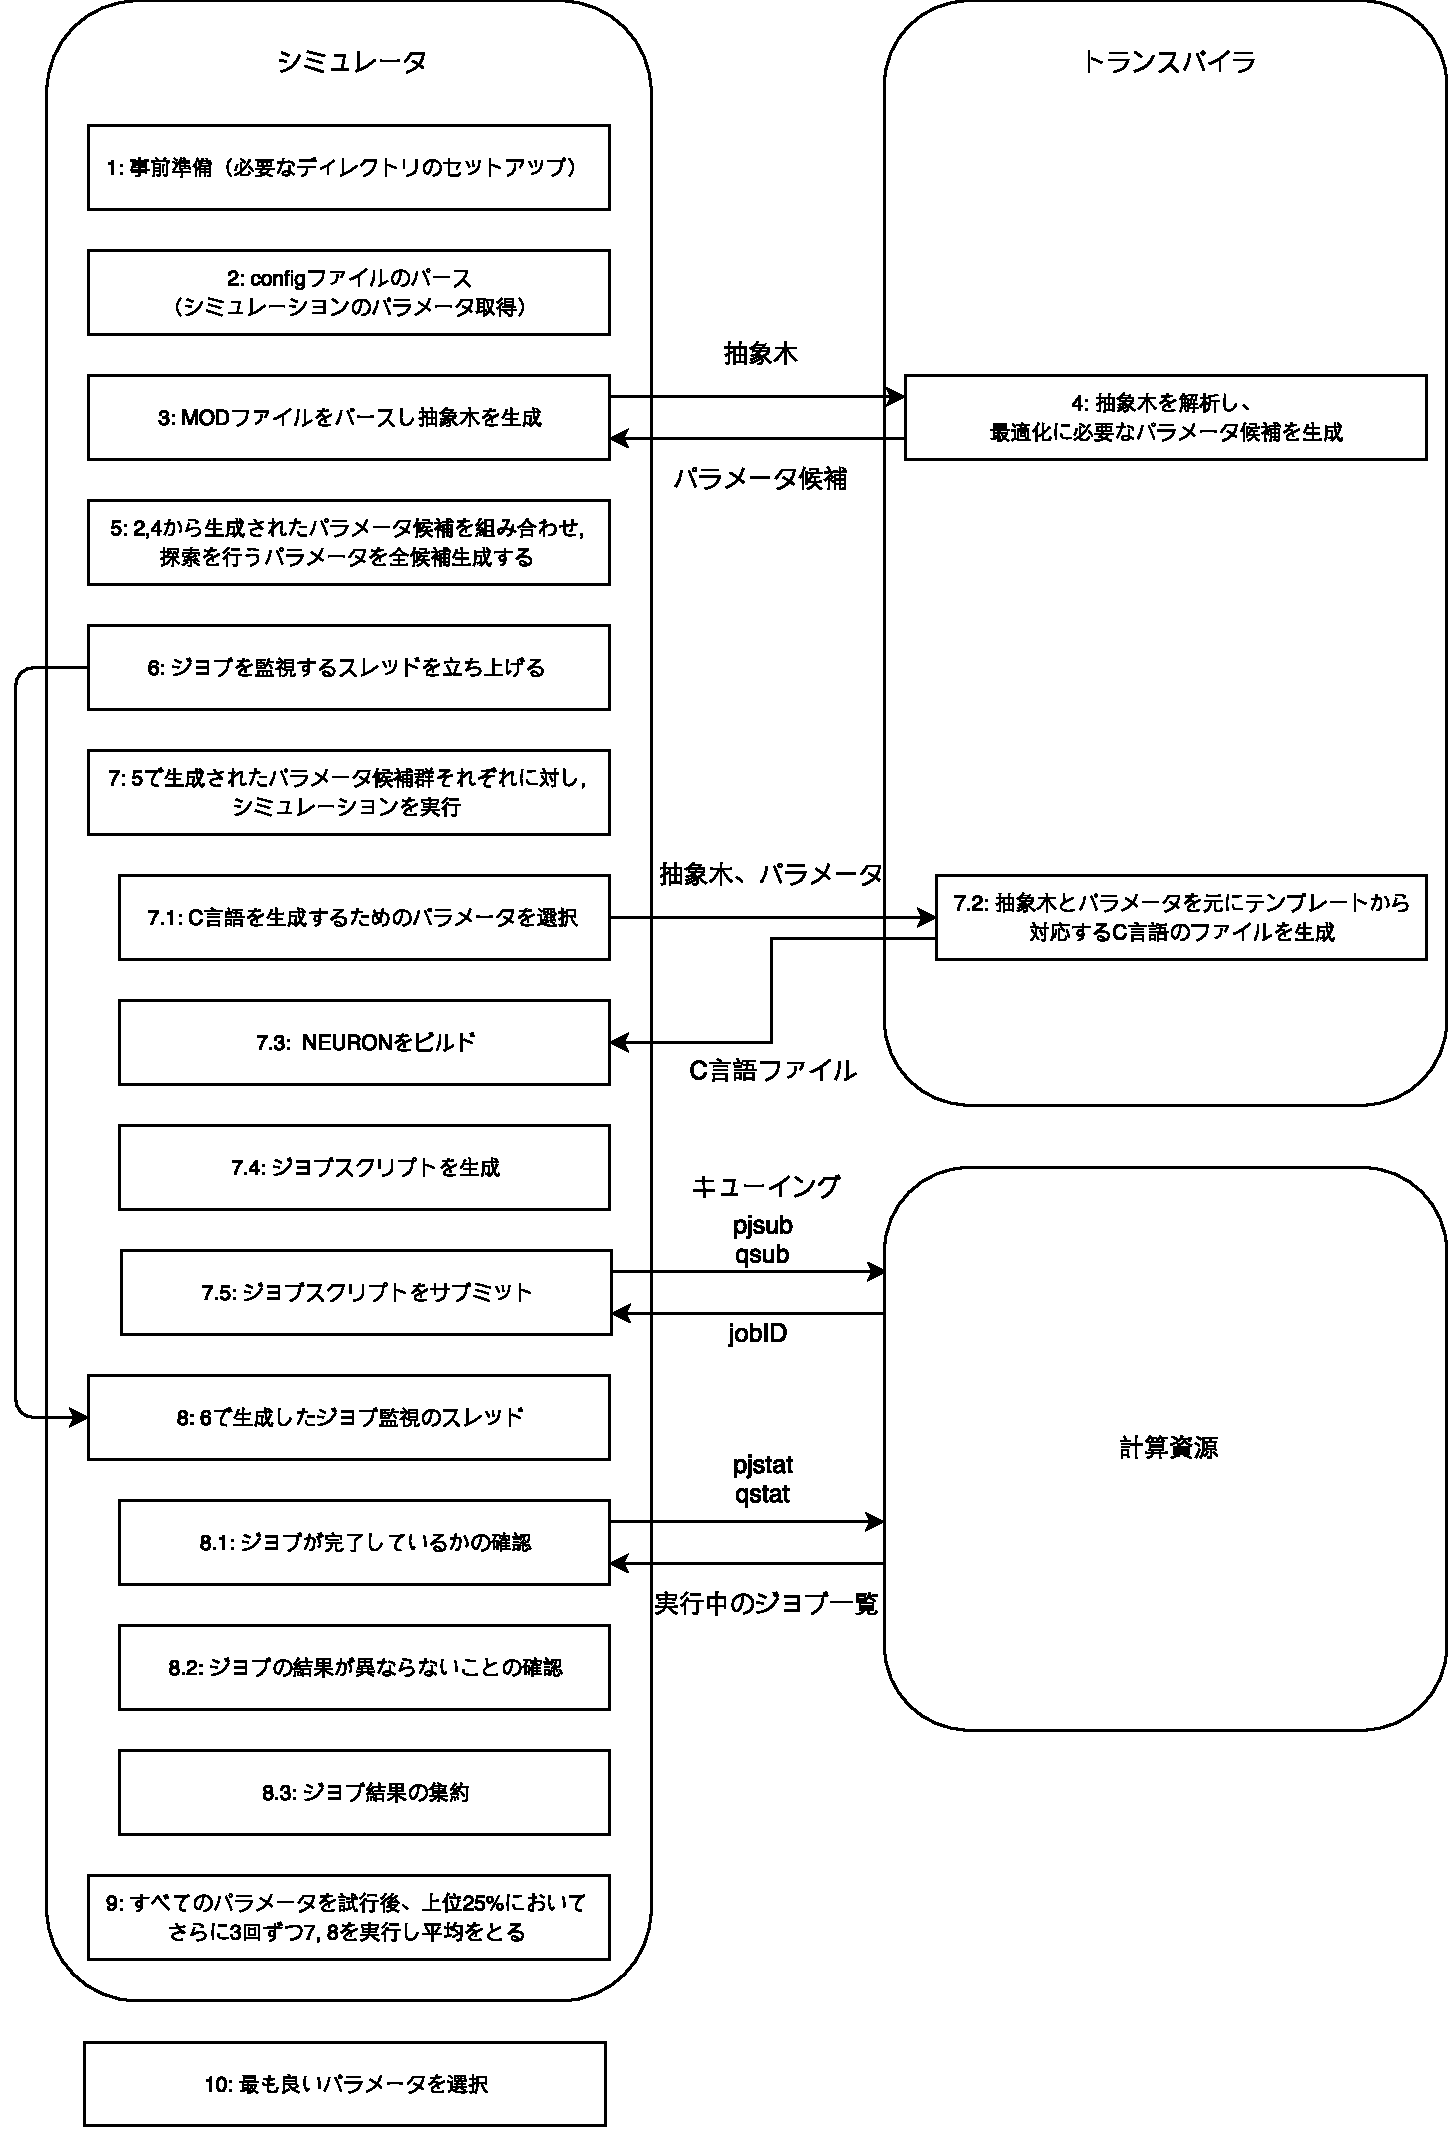
\includegraphics[width=18.0cm]{./images/Genie.pdf}
    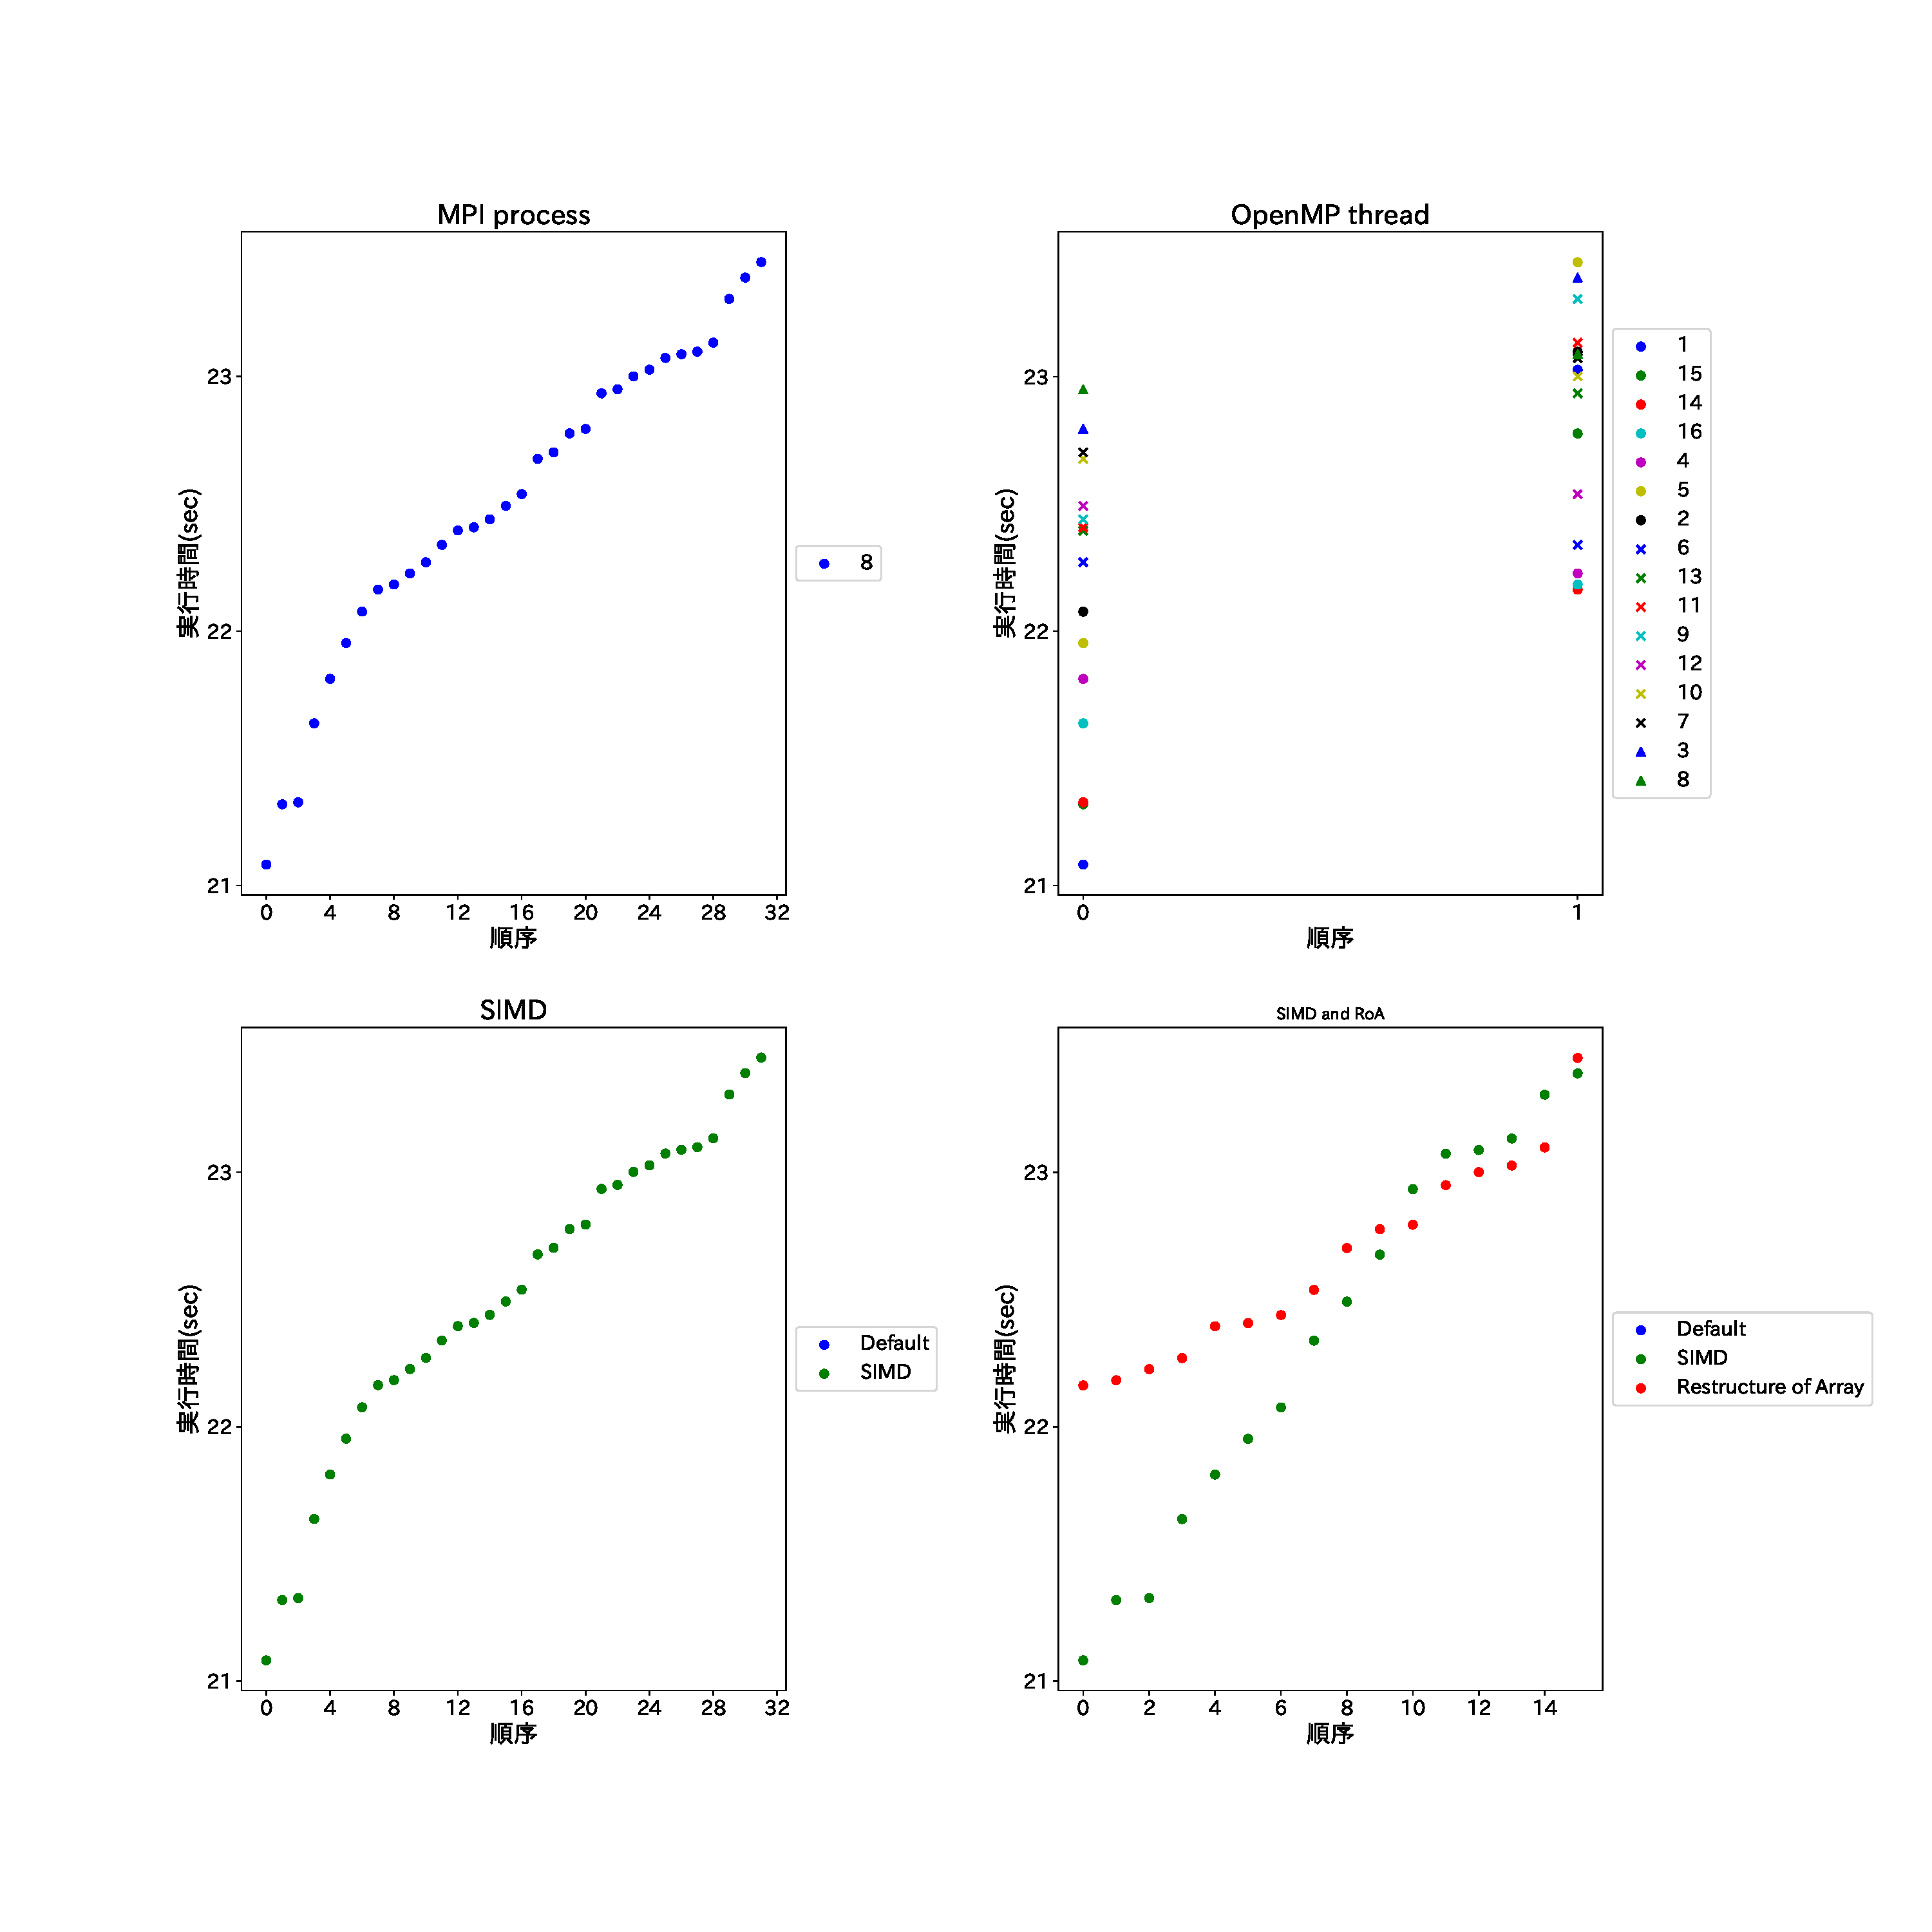
\includegraphics[width=14cm]{./images/k-bench-adjusted-final.pdf}
    \caption{京 小規模シミュレーション結果 パラメータ絞り込み後}
    \label{fig:k-bench-adjusted-final}
\end{center}
\end{figure}
\clearpage
次に小規模のシミュレーションを通して絞り込んだパラメータを用いて,
実行時間と反復する回数を変えてシミュレーションを再度行い,
実行時間とパラメータの関係を調べる.\\

\subsection{詳細なシミュレーションでのパラメータ比較}
\label{subsec:detail-sim}
ここでは\ref{subsec:small-sim}において絞り込みを行ったパラメータを用い,
京, クラスタそれぞれにおいて実行時間を50, 100, 250, 500, 1000msとして6回シミュレーションを行いその実行時間の平均をとることで,
より詳細にパラメータの比較を行った.
尚, SIMD化については\ref{subsec:small-sim}について既にSIMD化を行わないパラメータは除外されているためここでは触れない.\\

\subsubsection{MPIプロセス数}
\paragraph{クラスタ}~\\
図\ref{fig:cluster-mpi-process}のプロセス数に注目すると, プロセス数が28の時を除きシミュレーション時間を長くしてもMPIプロセス数間の関係に変化は見られない.\\
クラスタにおいてはコア数が28であることから,
シミュレーション時間が最大で1000msと短く細胞数も少ない今回のような場合においてはMPIプロセスでコアを埋めきるほうが計算性能が高くなることが読み取れる.\\
\begin{figure}[htb]
% h:here, t:top, b:bottom, p:page
\begin{center}
%    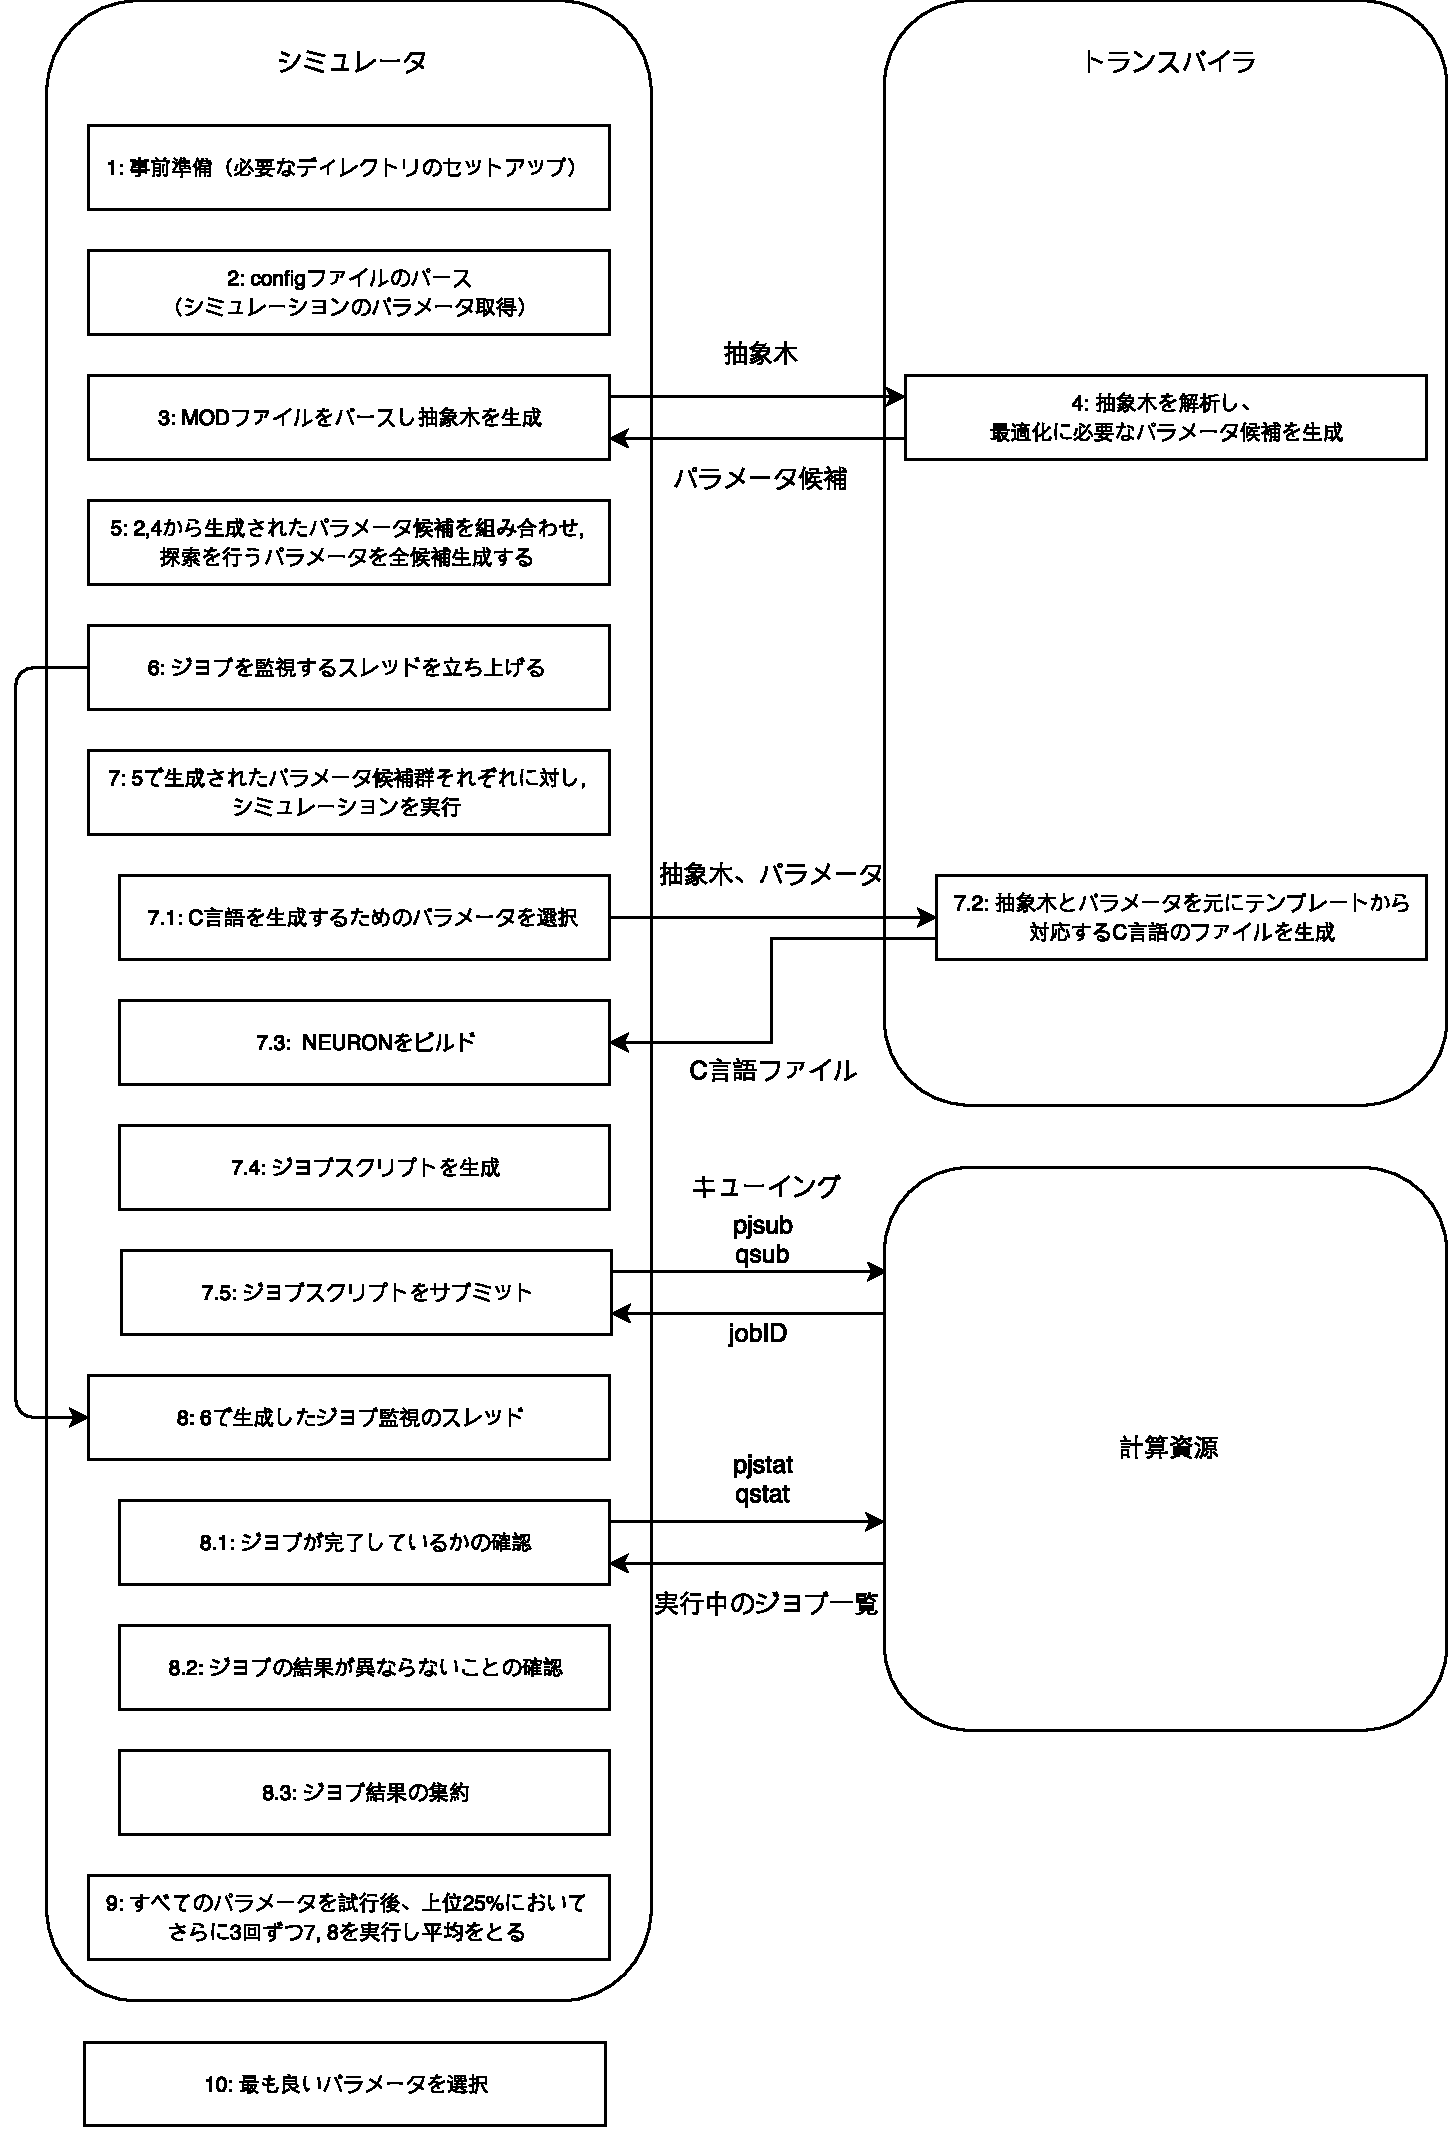
\includegraphics[width=18.0cm]{./images/Genie.pdf}
    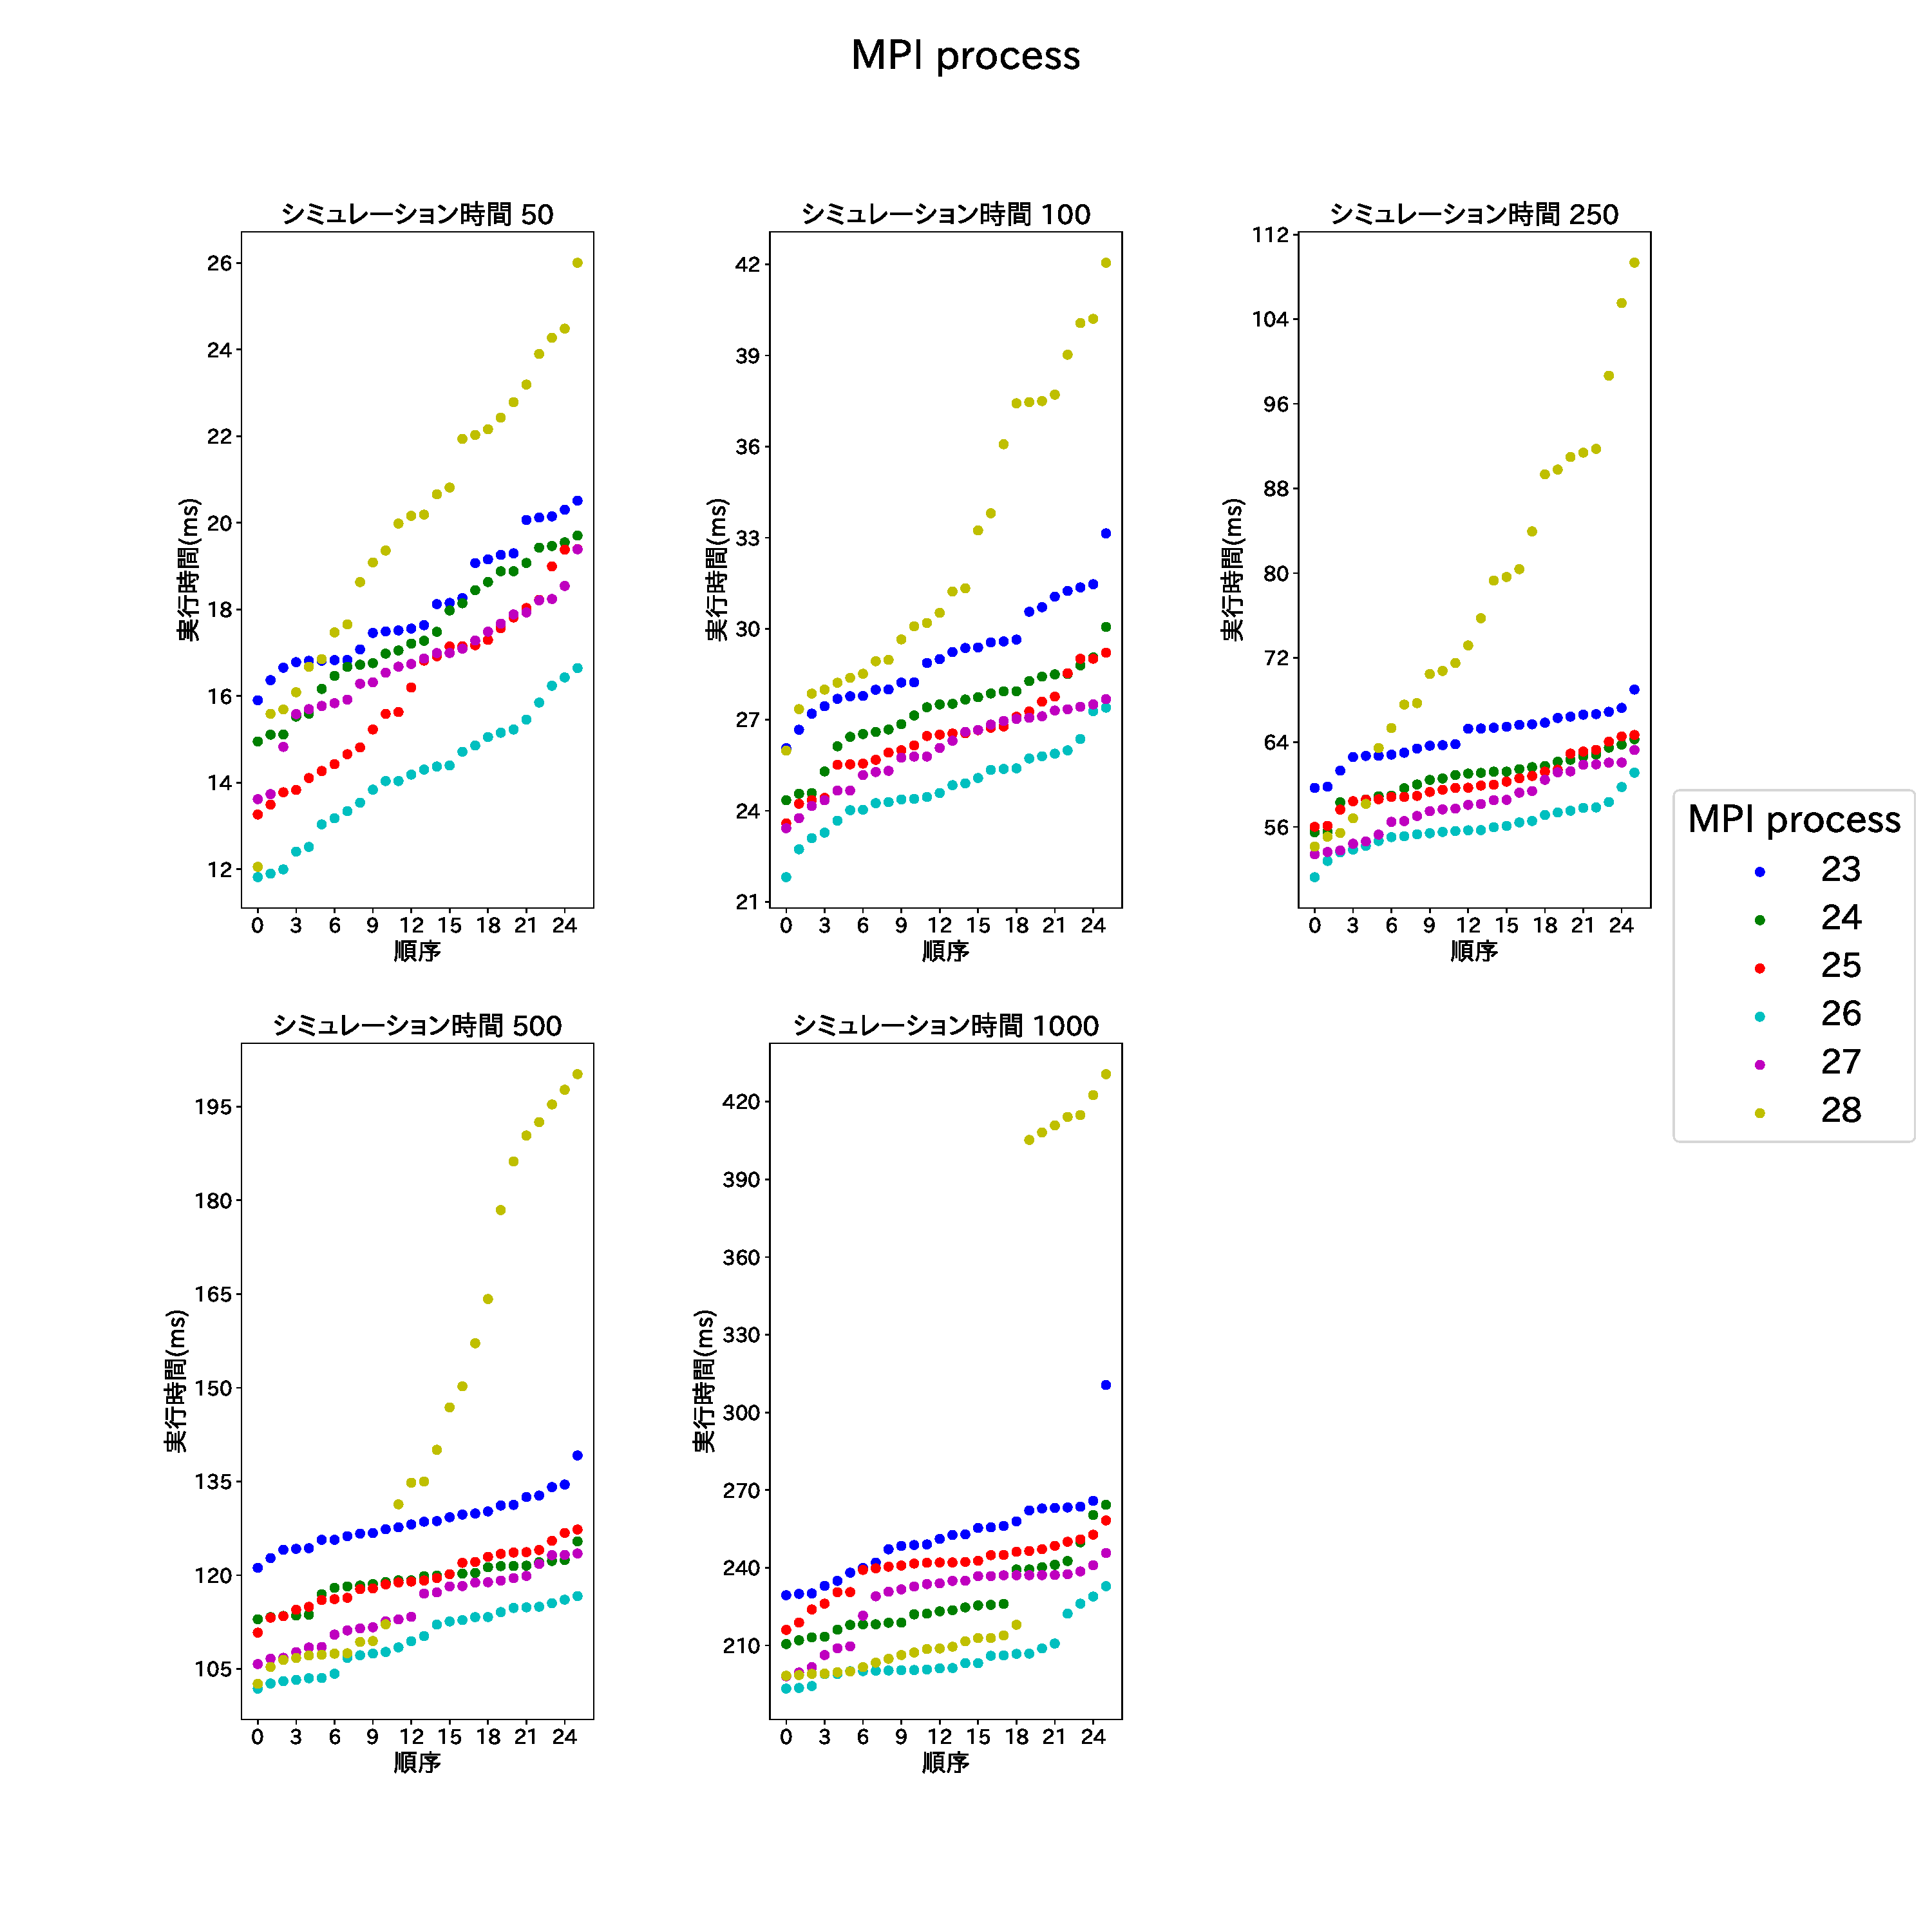
\includegraphics[width=12cm]{./images/cluster-MPI-process.pdf}
    \caption{クラスタ MPIプロセス数 シミュレーション結果}
    \label{fig:cluster-mpi-process}
\end{center}
\end{figure}
\clearpage

\paragraph{京}~\\
% \begin{figure}[htb]
% % h:here, t:top, b:bottom, p:page
% \begin{center}
% %    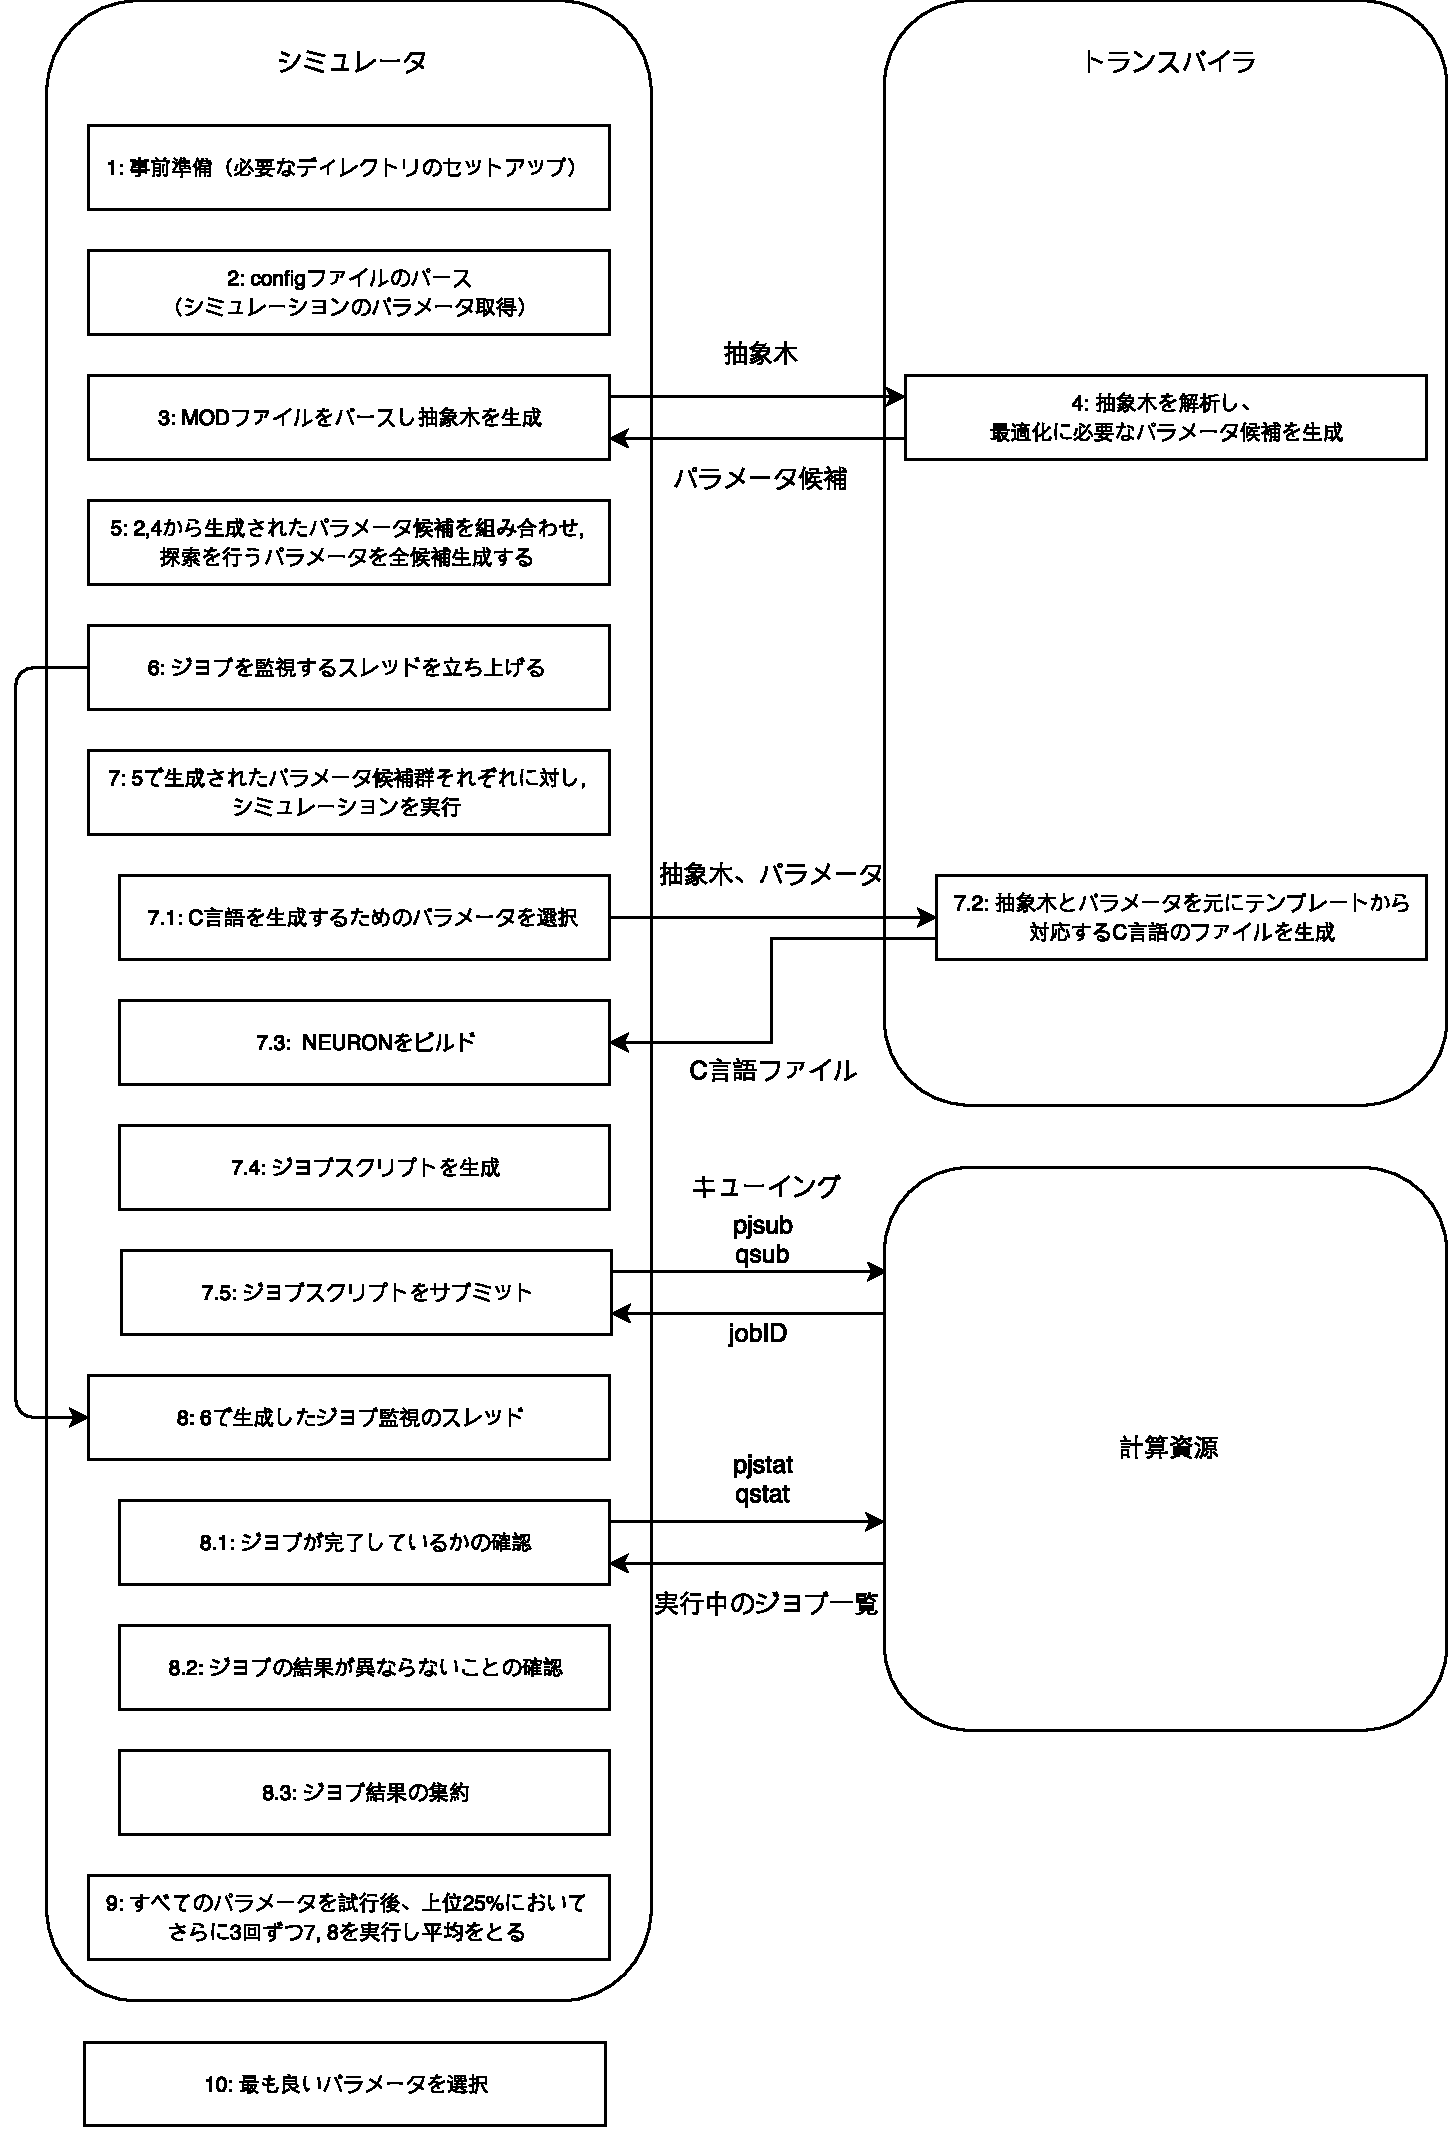
\includegraphics[width=18.0cm]{./images/Genie.pdf}
%     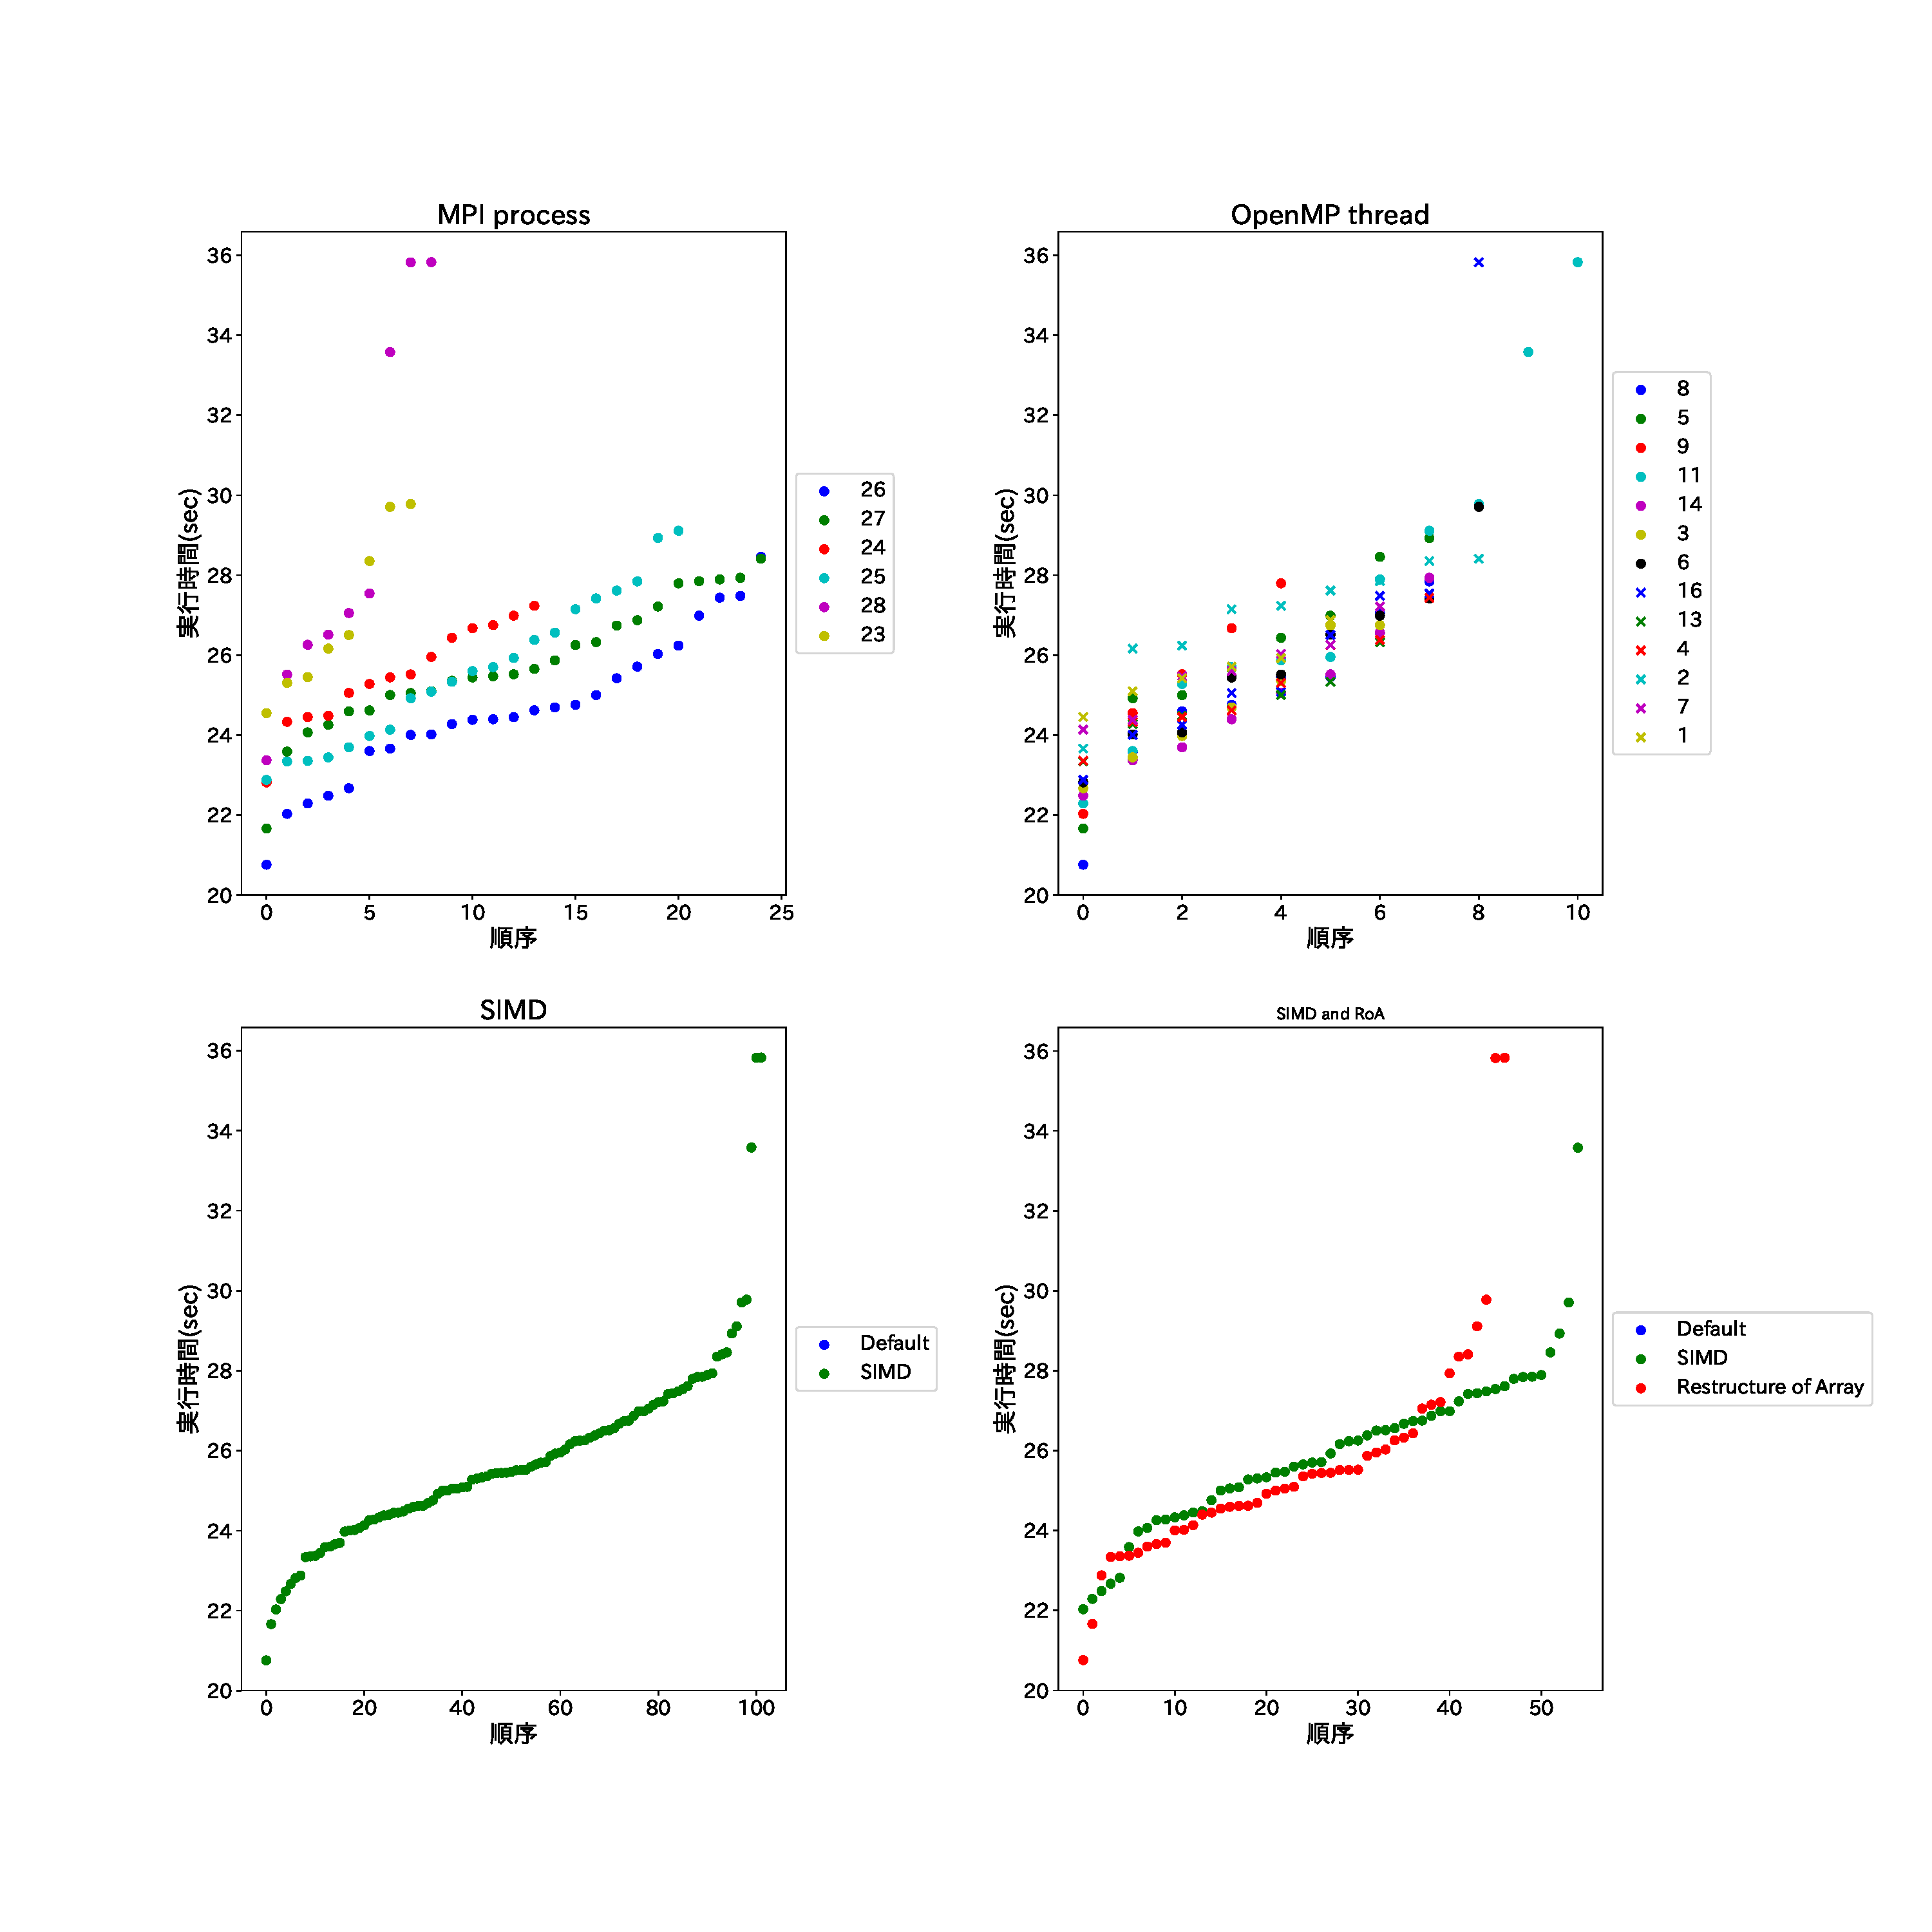
\includegraphics[width=14cm]{./images/cluster-bench-adjusted-final.pdf}
%     \caption{クラスタ 小規模シミュレーション結果 パラメータ絞り込み後}
%     \label{fig:cluster-bench-adjusted-final}
% \end{center}
% \end{figure}
% \clearpage

\subsubsection{OpenMPスレッド数}
\paragraph{クラスタ}~\\
OpenMPスレッドについては他のパラメータと違いスレッド数の間で大きな差が見られない傾向にあったため,
図\ref{fig:cluster-openmp}のように折れ線グラフを用いてどの程度混在しているのか確認した.\\

\begin{figure}[htb]
% h:here, t:top, b:bottom, p:page
\begin{center}
%    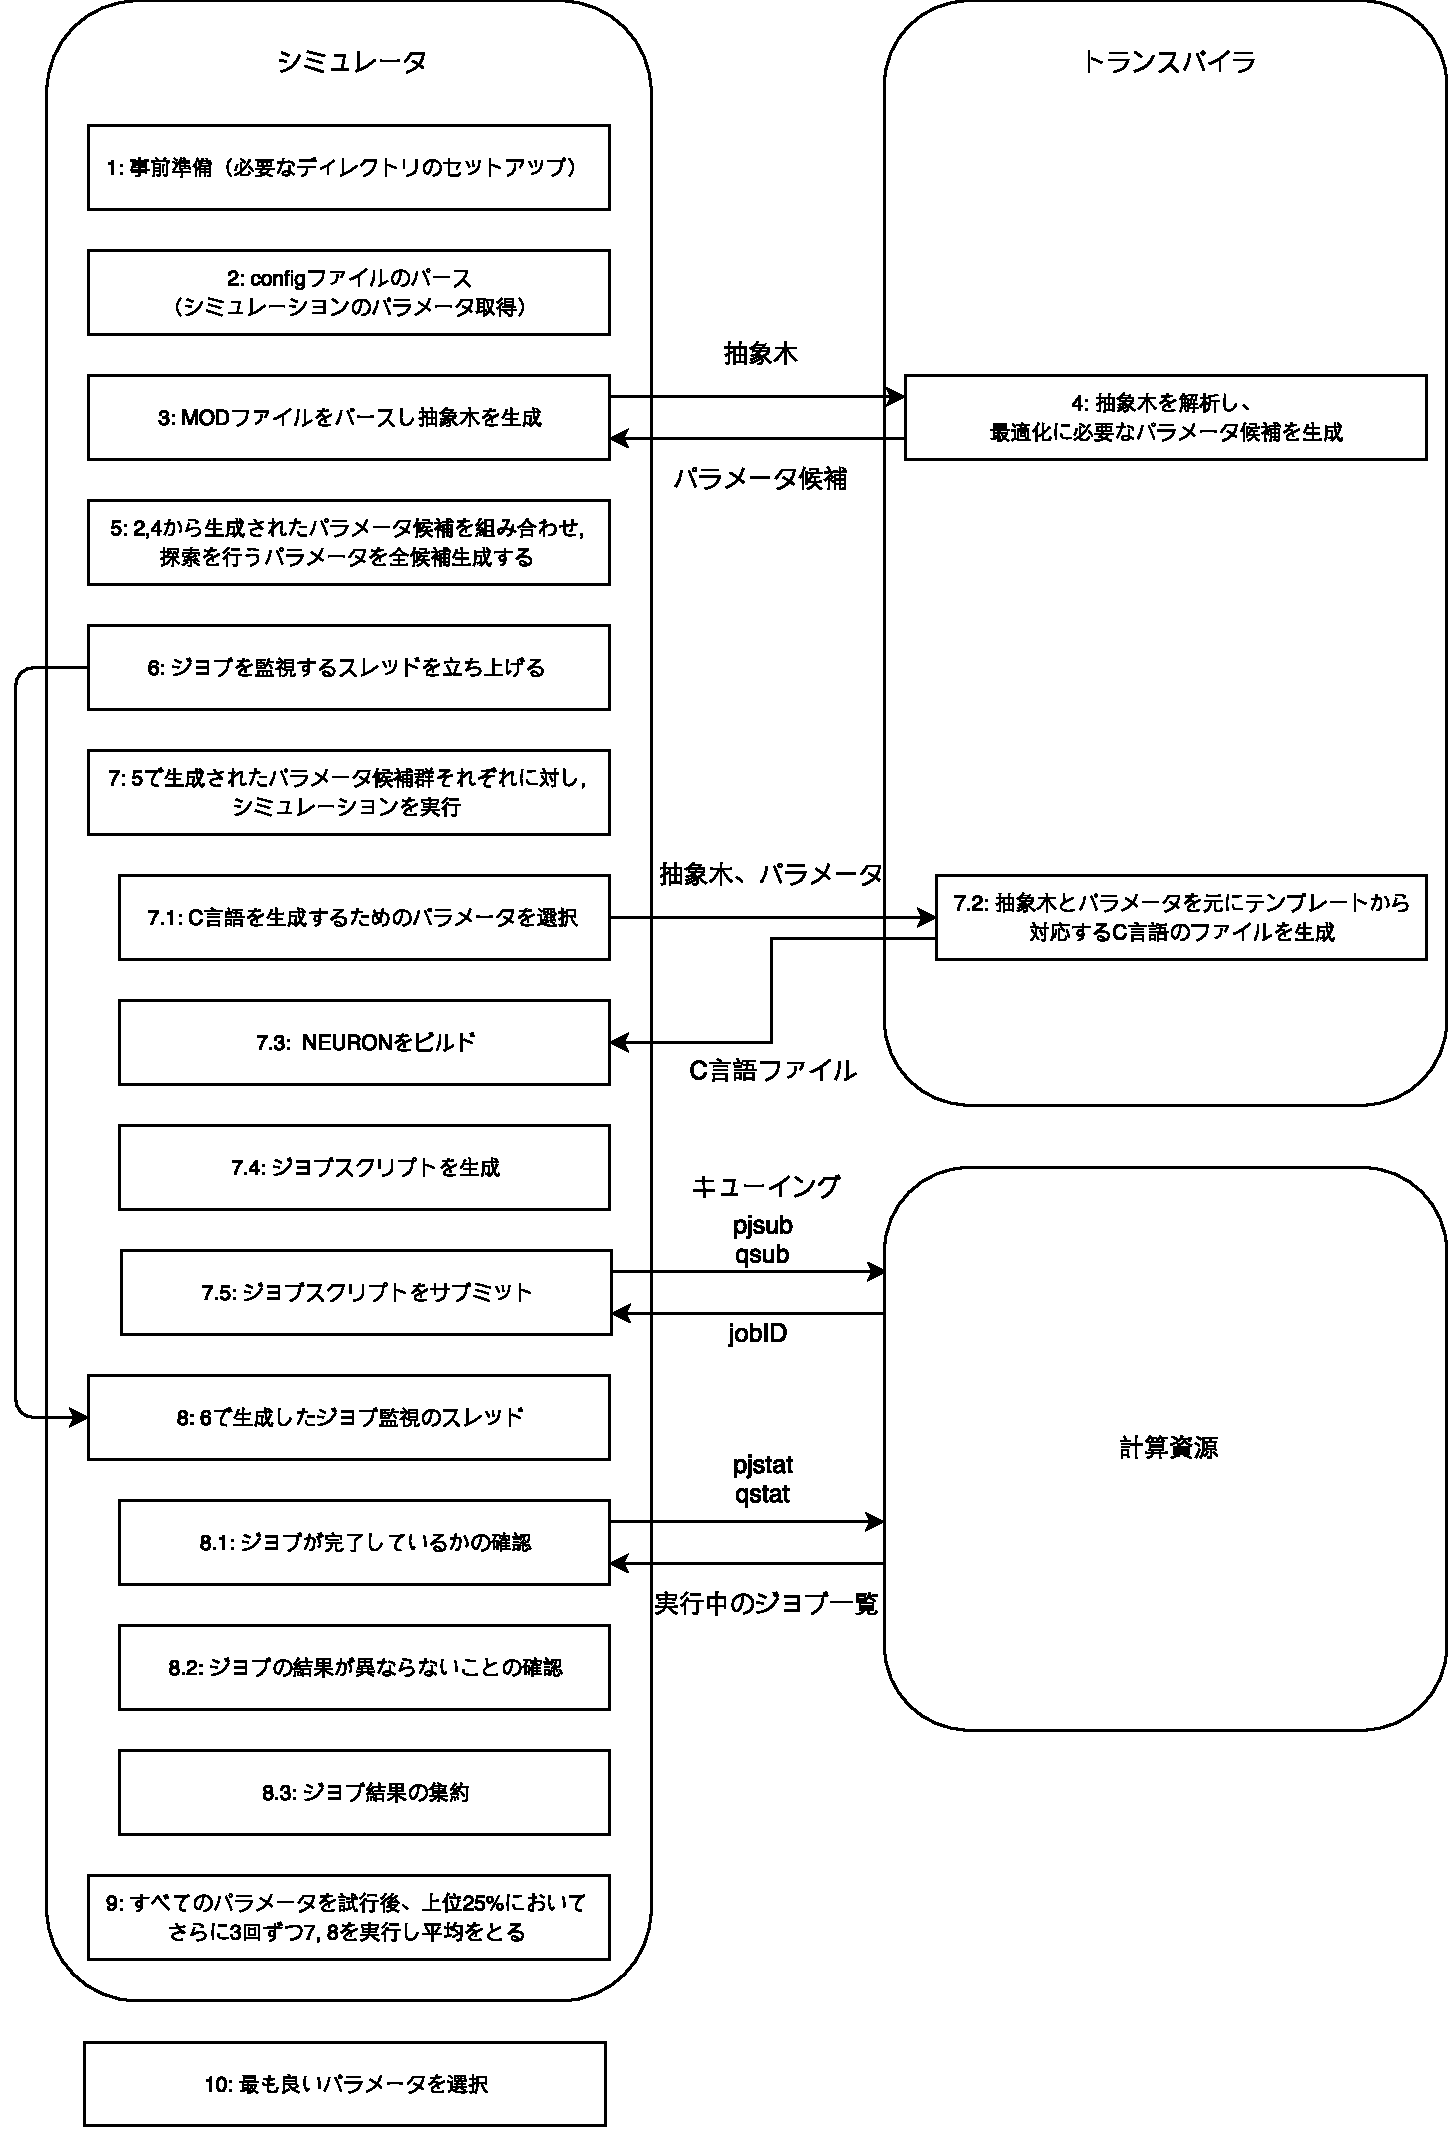
\includegraphics[width=18.0cm]{./images/Genie.pdf}
    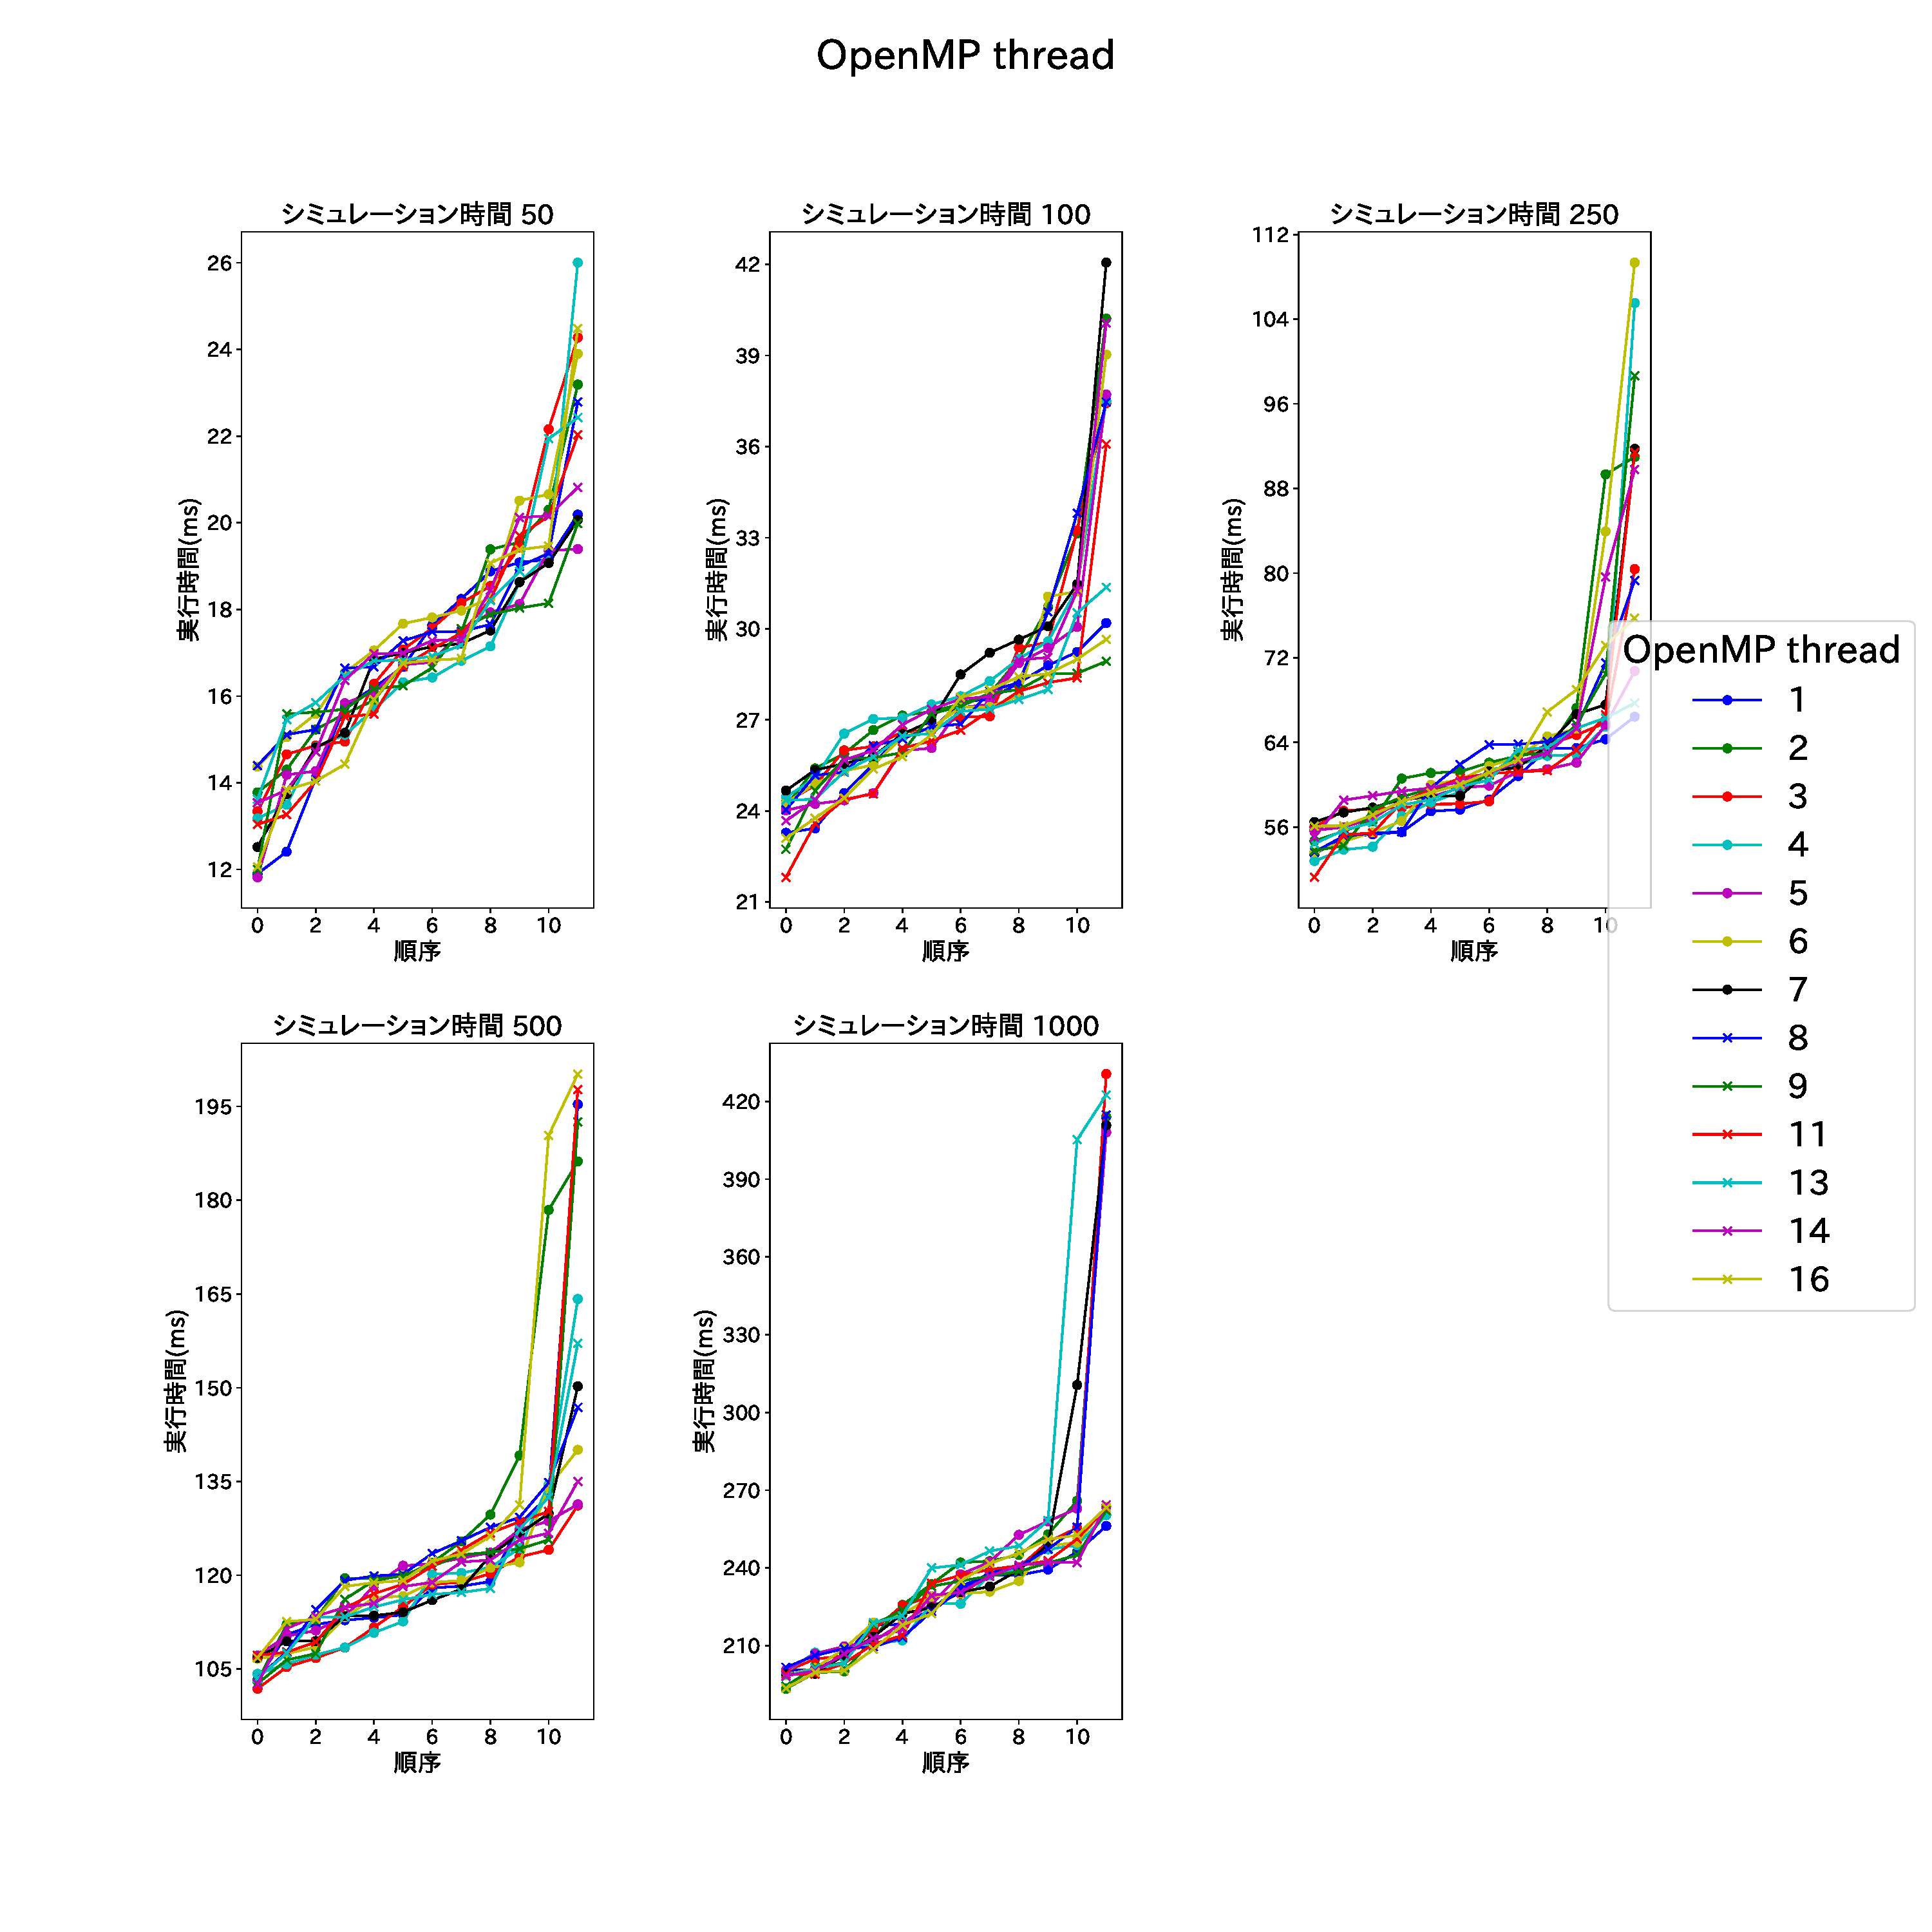
\includegraphics[width=14cm]{./images/cluster-OpenMP-thread.pdf}
    \caption{クラスタ OpenMPスレッド数 シミュレーション結果}
    \label{fig:cluster-openmp}
\end{center}
\end{figure}

図\ref{fig:cluster-openmp}において表示されるデータ点が多すぎるため,
データ点の数を50個に制限したものを次の図\ref{fig:cluster-openmp-top50}に示す.\\
\begin{figure}[htb]
% h:here, t:top, b:bottom, p:page
\begin{center}
%    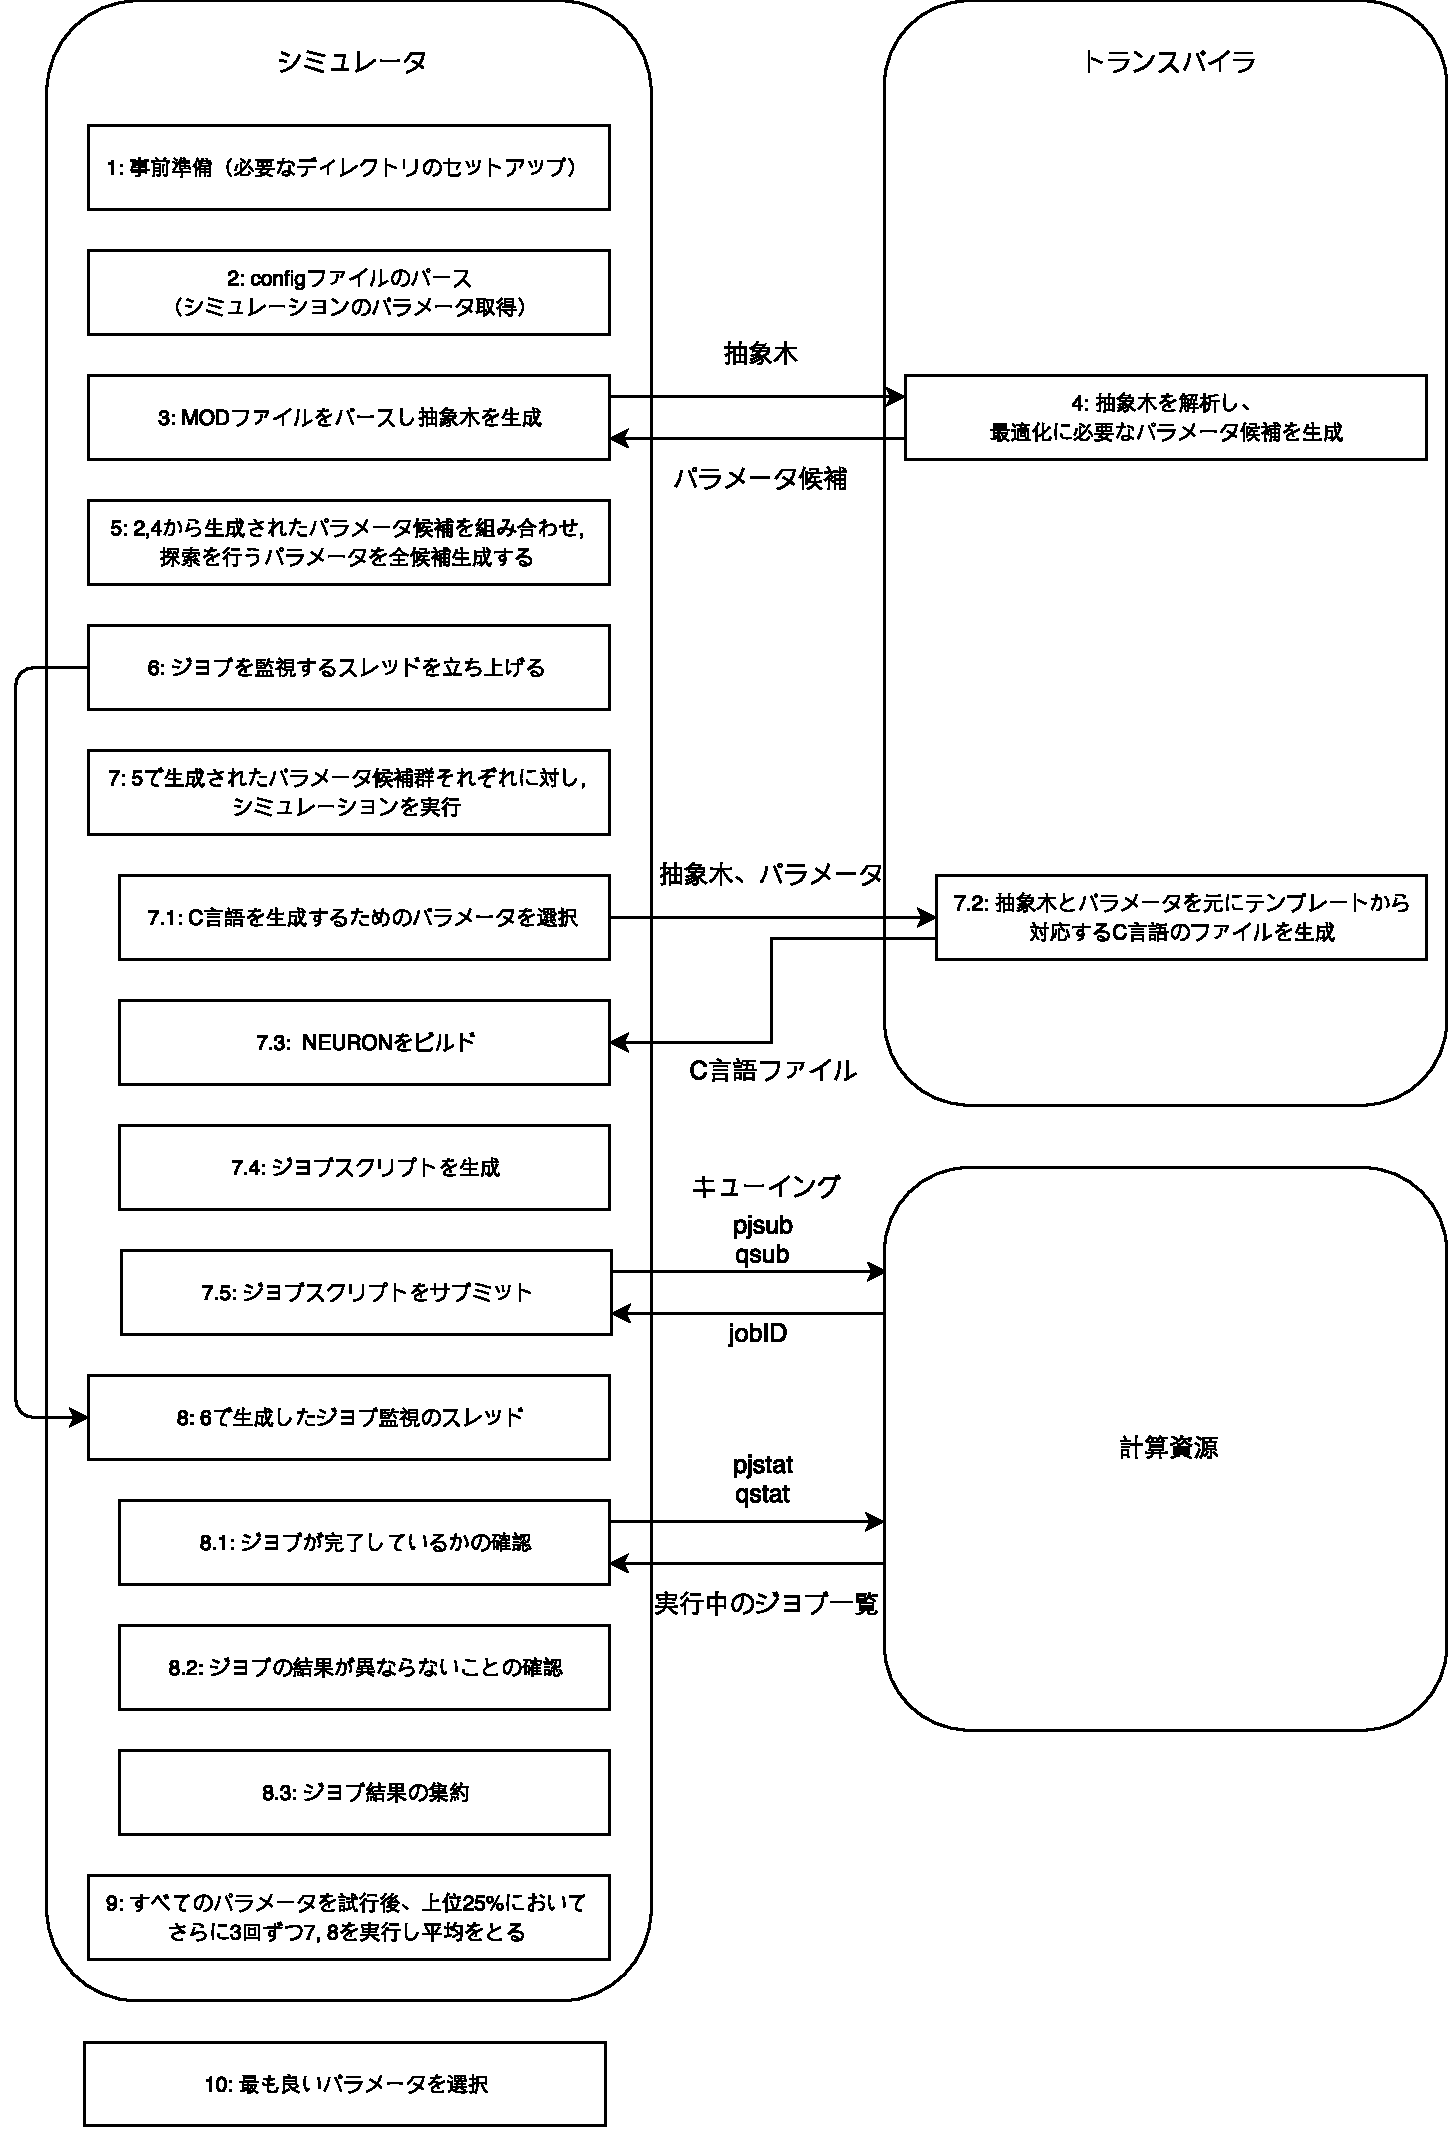
\includegraphics[width=18.0cm]{./images/Genie.pdf}
    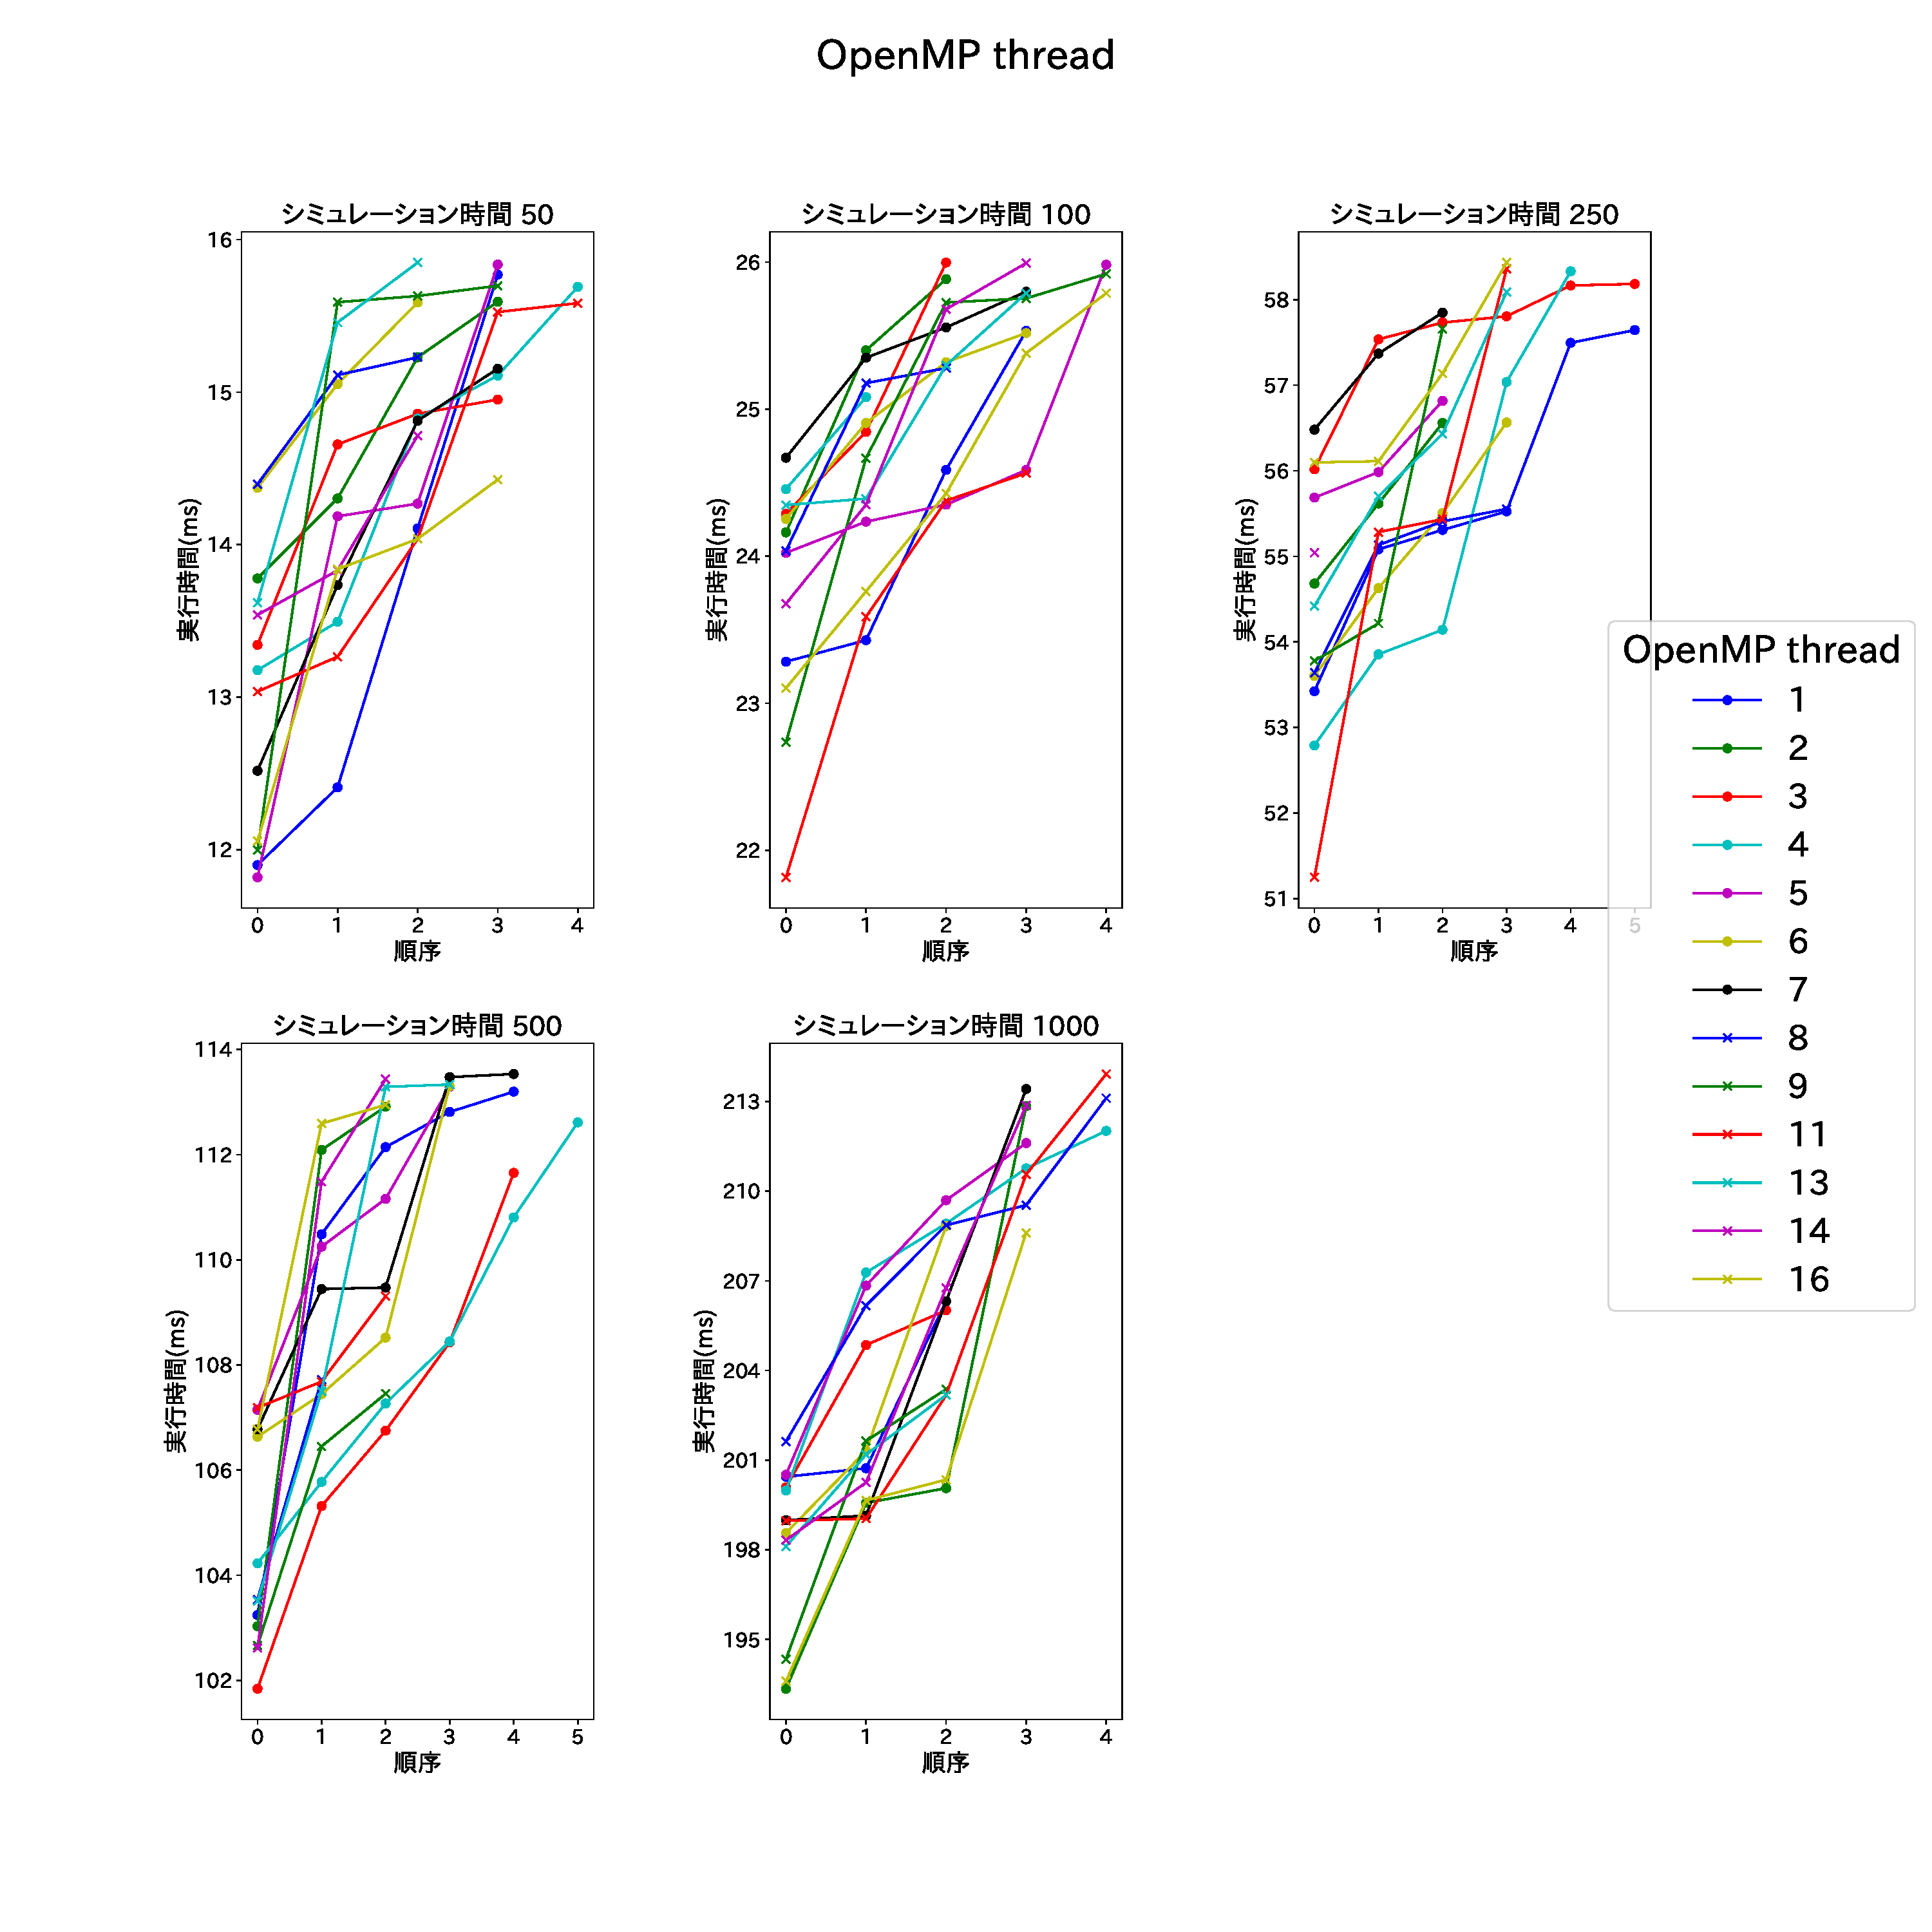
\includegraphics[width=14cm]{./images/cluster-top50-OpenMP-thread.pdf}
    \caption{クラスタ OpenMPスレッド数 シミュレーション結果 上位50組}
    \label{fig:cluster-openmp-top50}
\end{center}
\end{figure}

結果として, データ点を制限して表示した図においてもスレッド数と実行時間の直接的な相関を見ることができなかった.
これは\ref{subsubsec:hybrid}において述べたMPIとOpenMPのハイブリッドという観点では,
シミュレーションの規模が小さくMPIプロセスが通信に用いるリソースが十分に存在したため,
MPIによってコアを埋めた後ではOpenMPのスレッド数をいくつに設定しても実行時間に与える影響が少ないためだと考えられる.\\
\clearpage

\paragraph{京}~\\
% \begin{figure}[htb]
% % h:here, t:top, b:bottom, p:page
% \begin{center}
% %    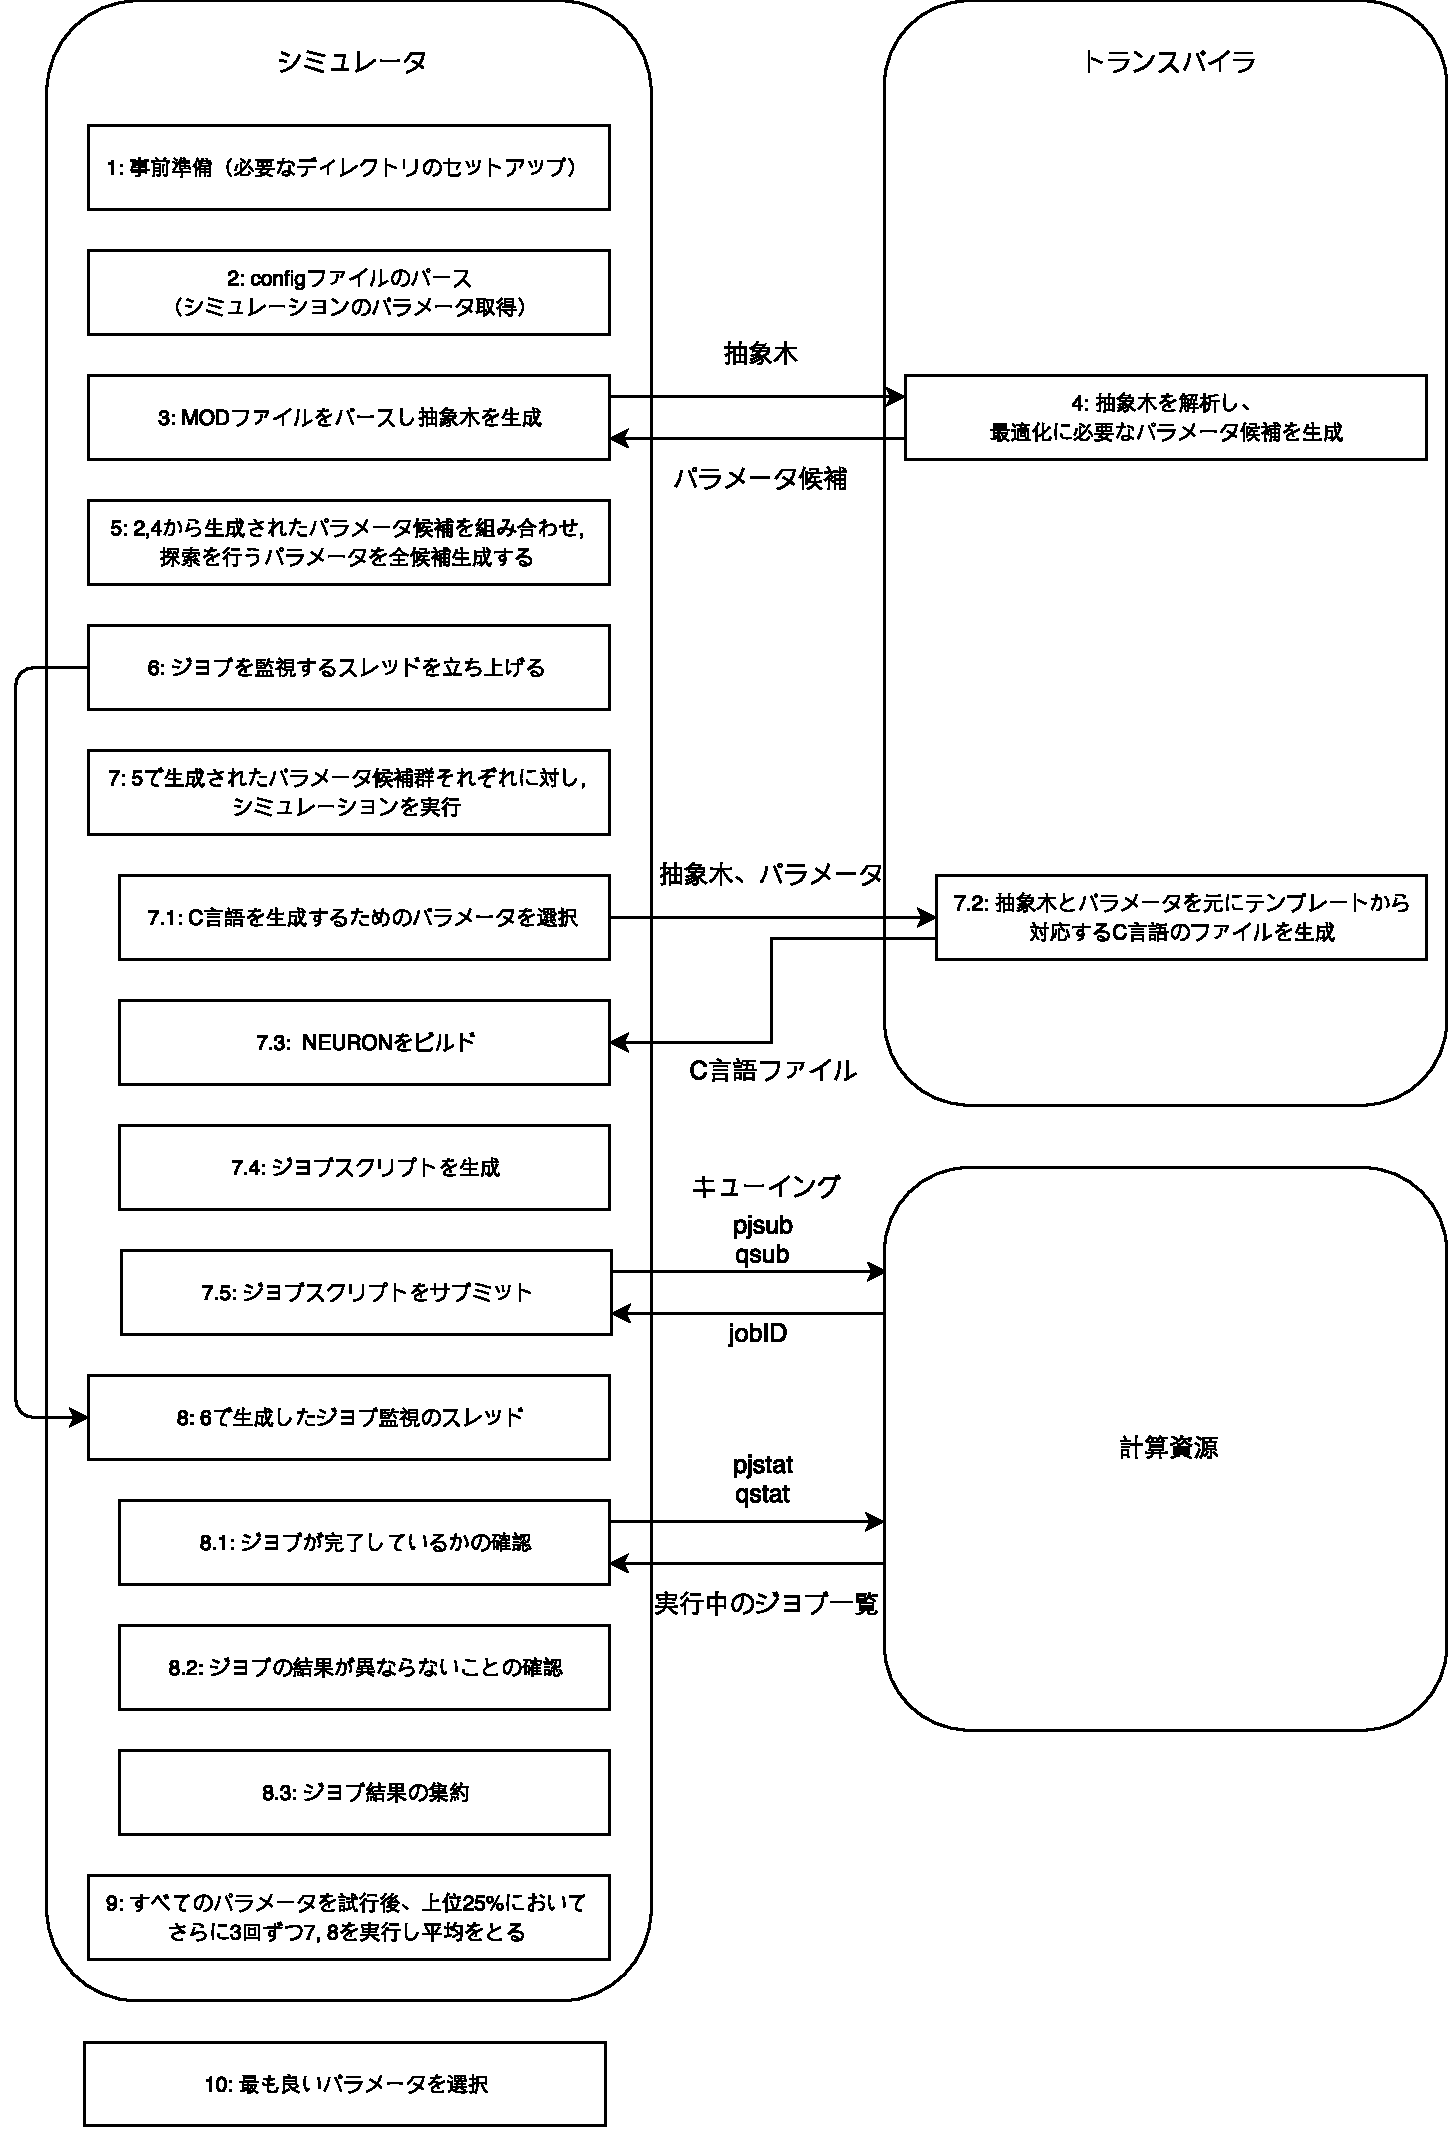
\includegraphics[width=18.0cm]{./images/Genie.pdf}
%     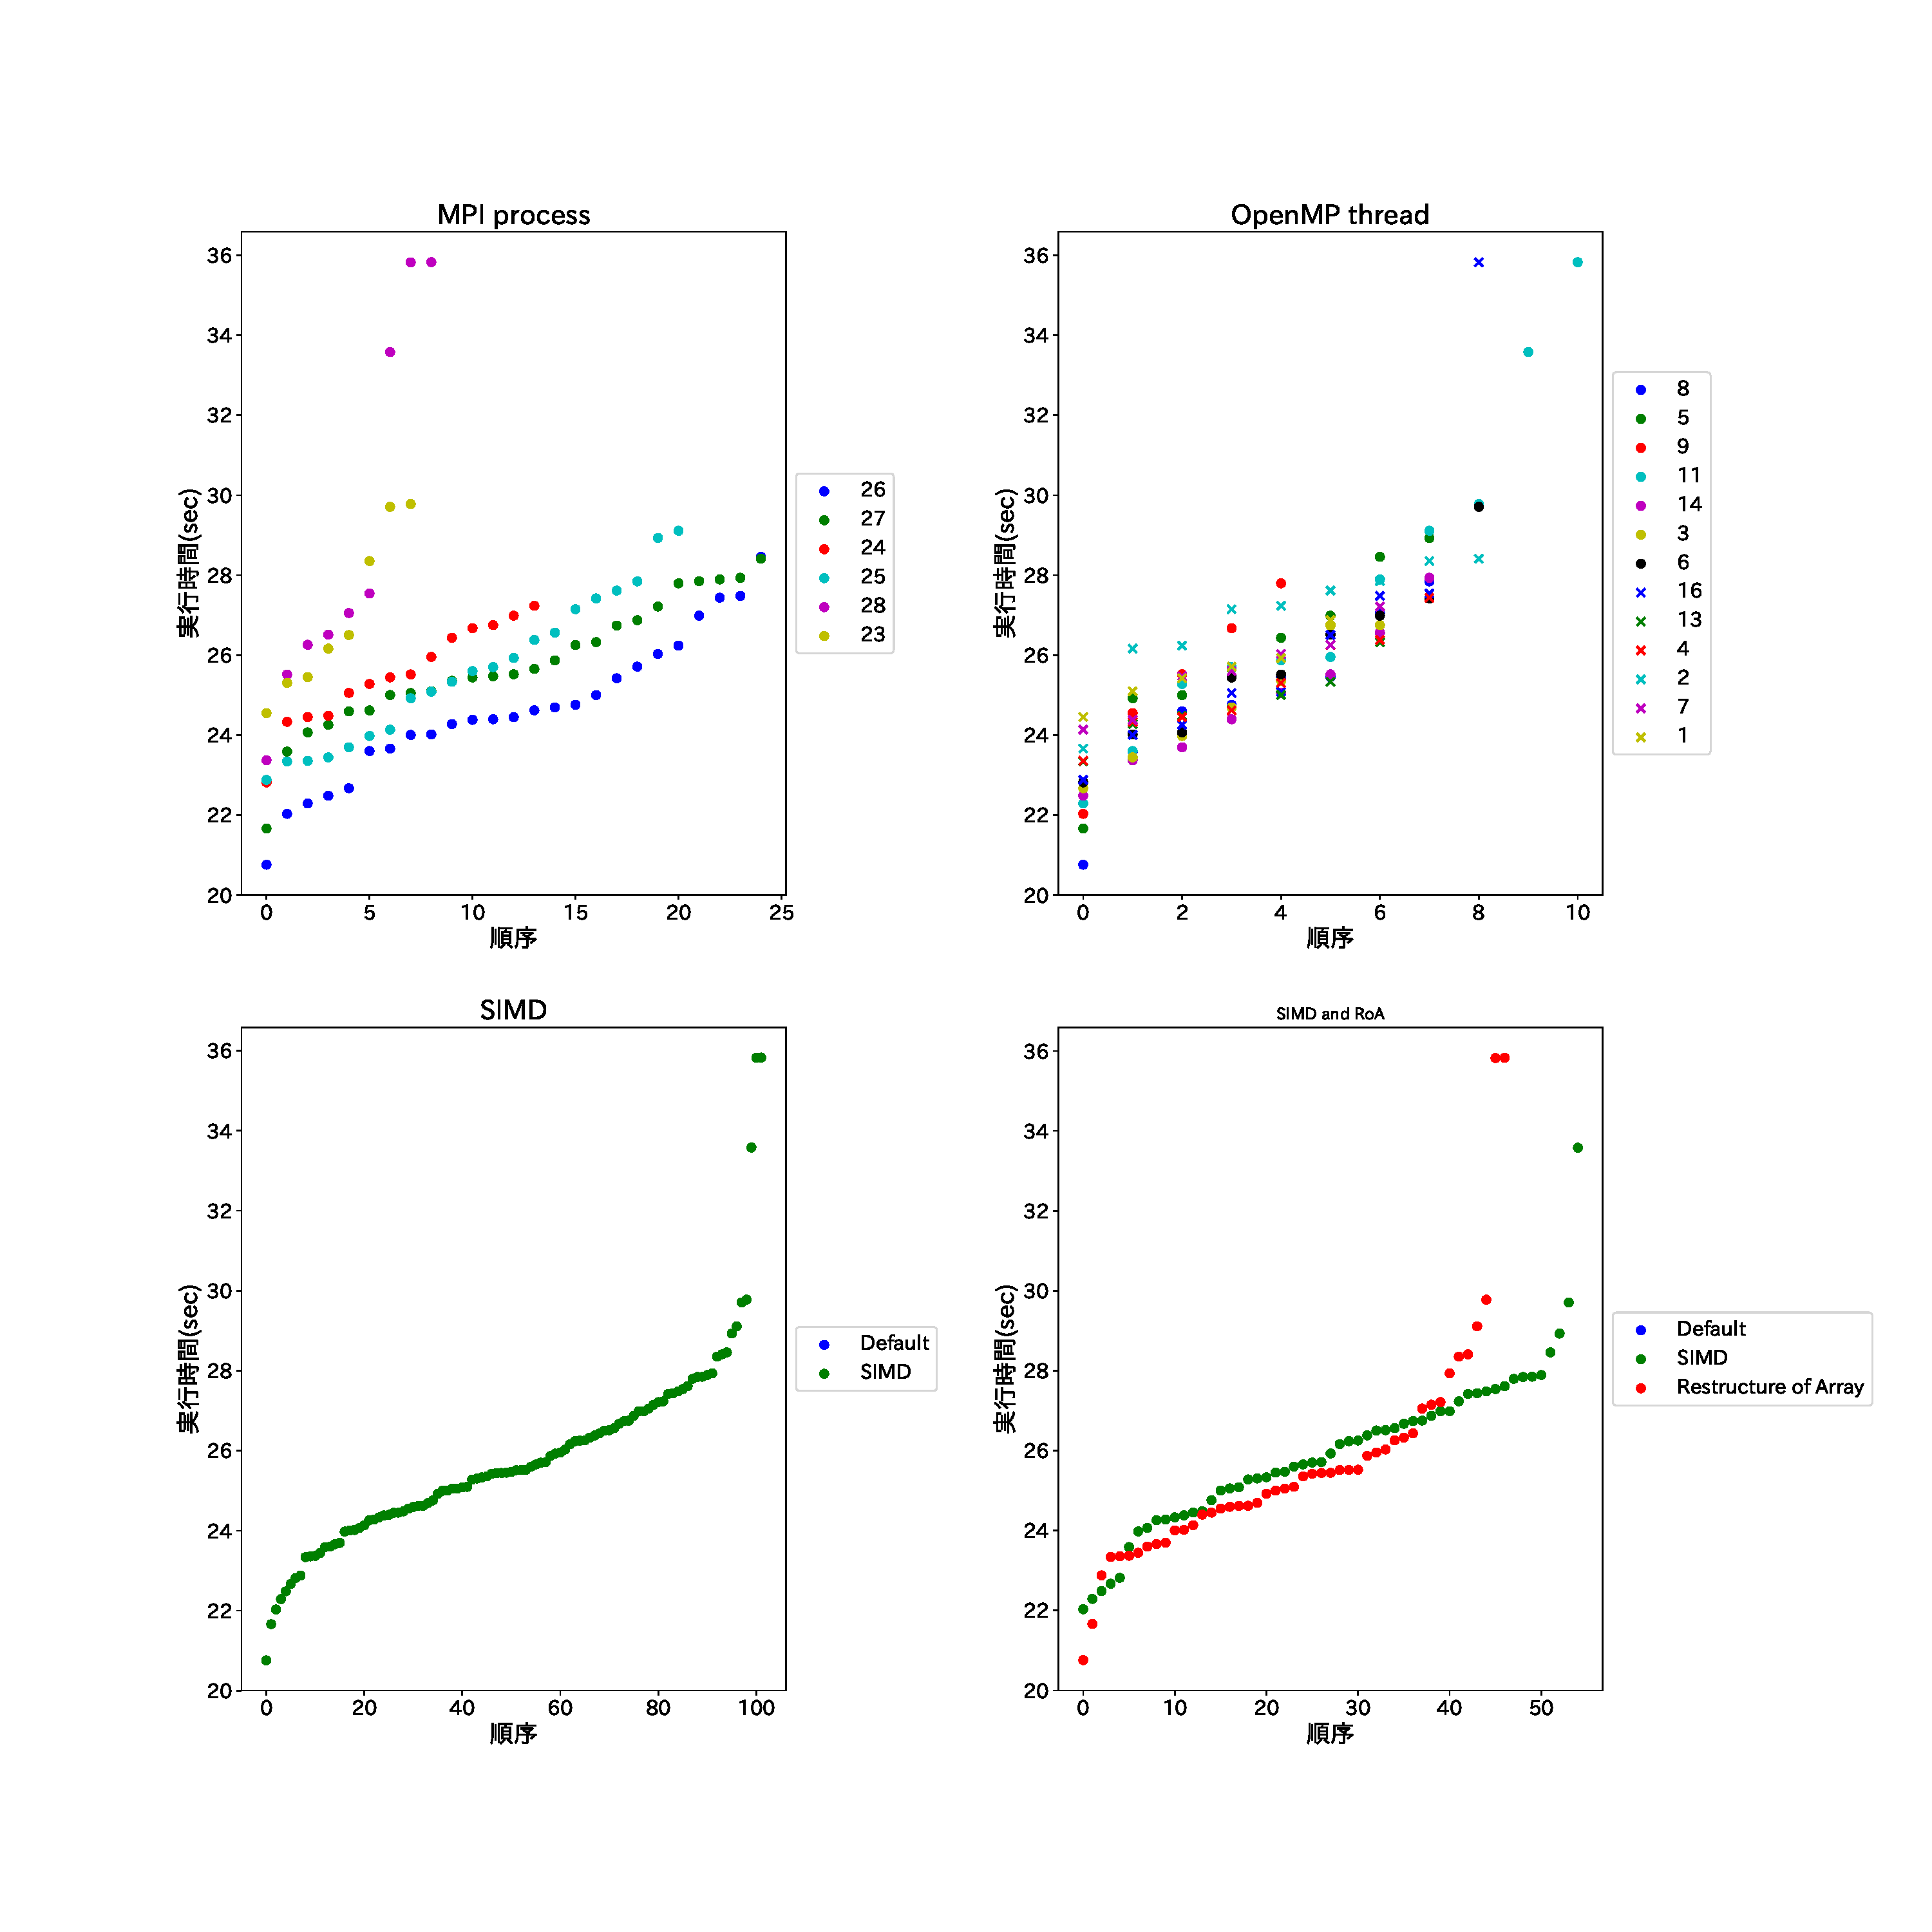
\includegraphics[width=14cm]{./images/cluster-bench-adjusted-final.pdf}
%     \caption{クラスタ 小規模シミュレーション結果 パラメータ絞り込み後}
%     \label{fig:cluster-bench-adjusted-final}
% \end{center}
% \end{figure}
% \clearpage

\subsubsection{配列のくくり出し}
\paragraph{クラスタ}~\\
変数の配列化を通してコンパイラによるSIMD化を促進することで計算能力が大きく向上することは,
前節の結果から読み取れる. ここでは配列化を行った変数に対してさらにくくり出しを行った場合と行わなかった場合を比較する.\\
また図\ref{fig:cluster-roa}において実行時間が早い前半部分が潰れてしまっているため,
図\ref{fig:cluster-roa-top50}に他のパラメータと同じく拡大した図を示す.\\
\begin{figure}[htb]
% h:here, t:top, b:bottom, p:page
\begin{center}
%    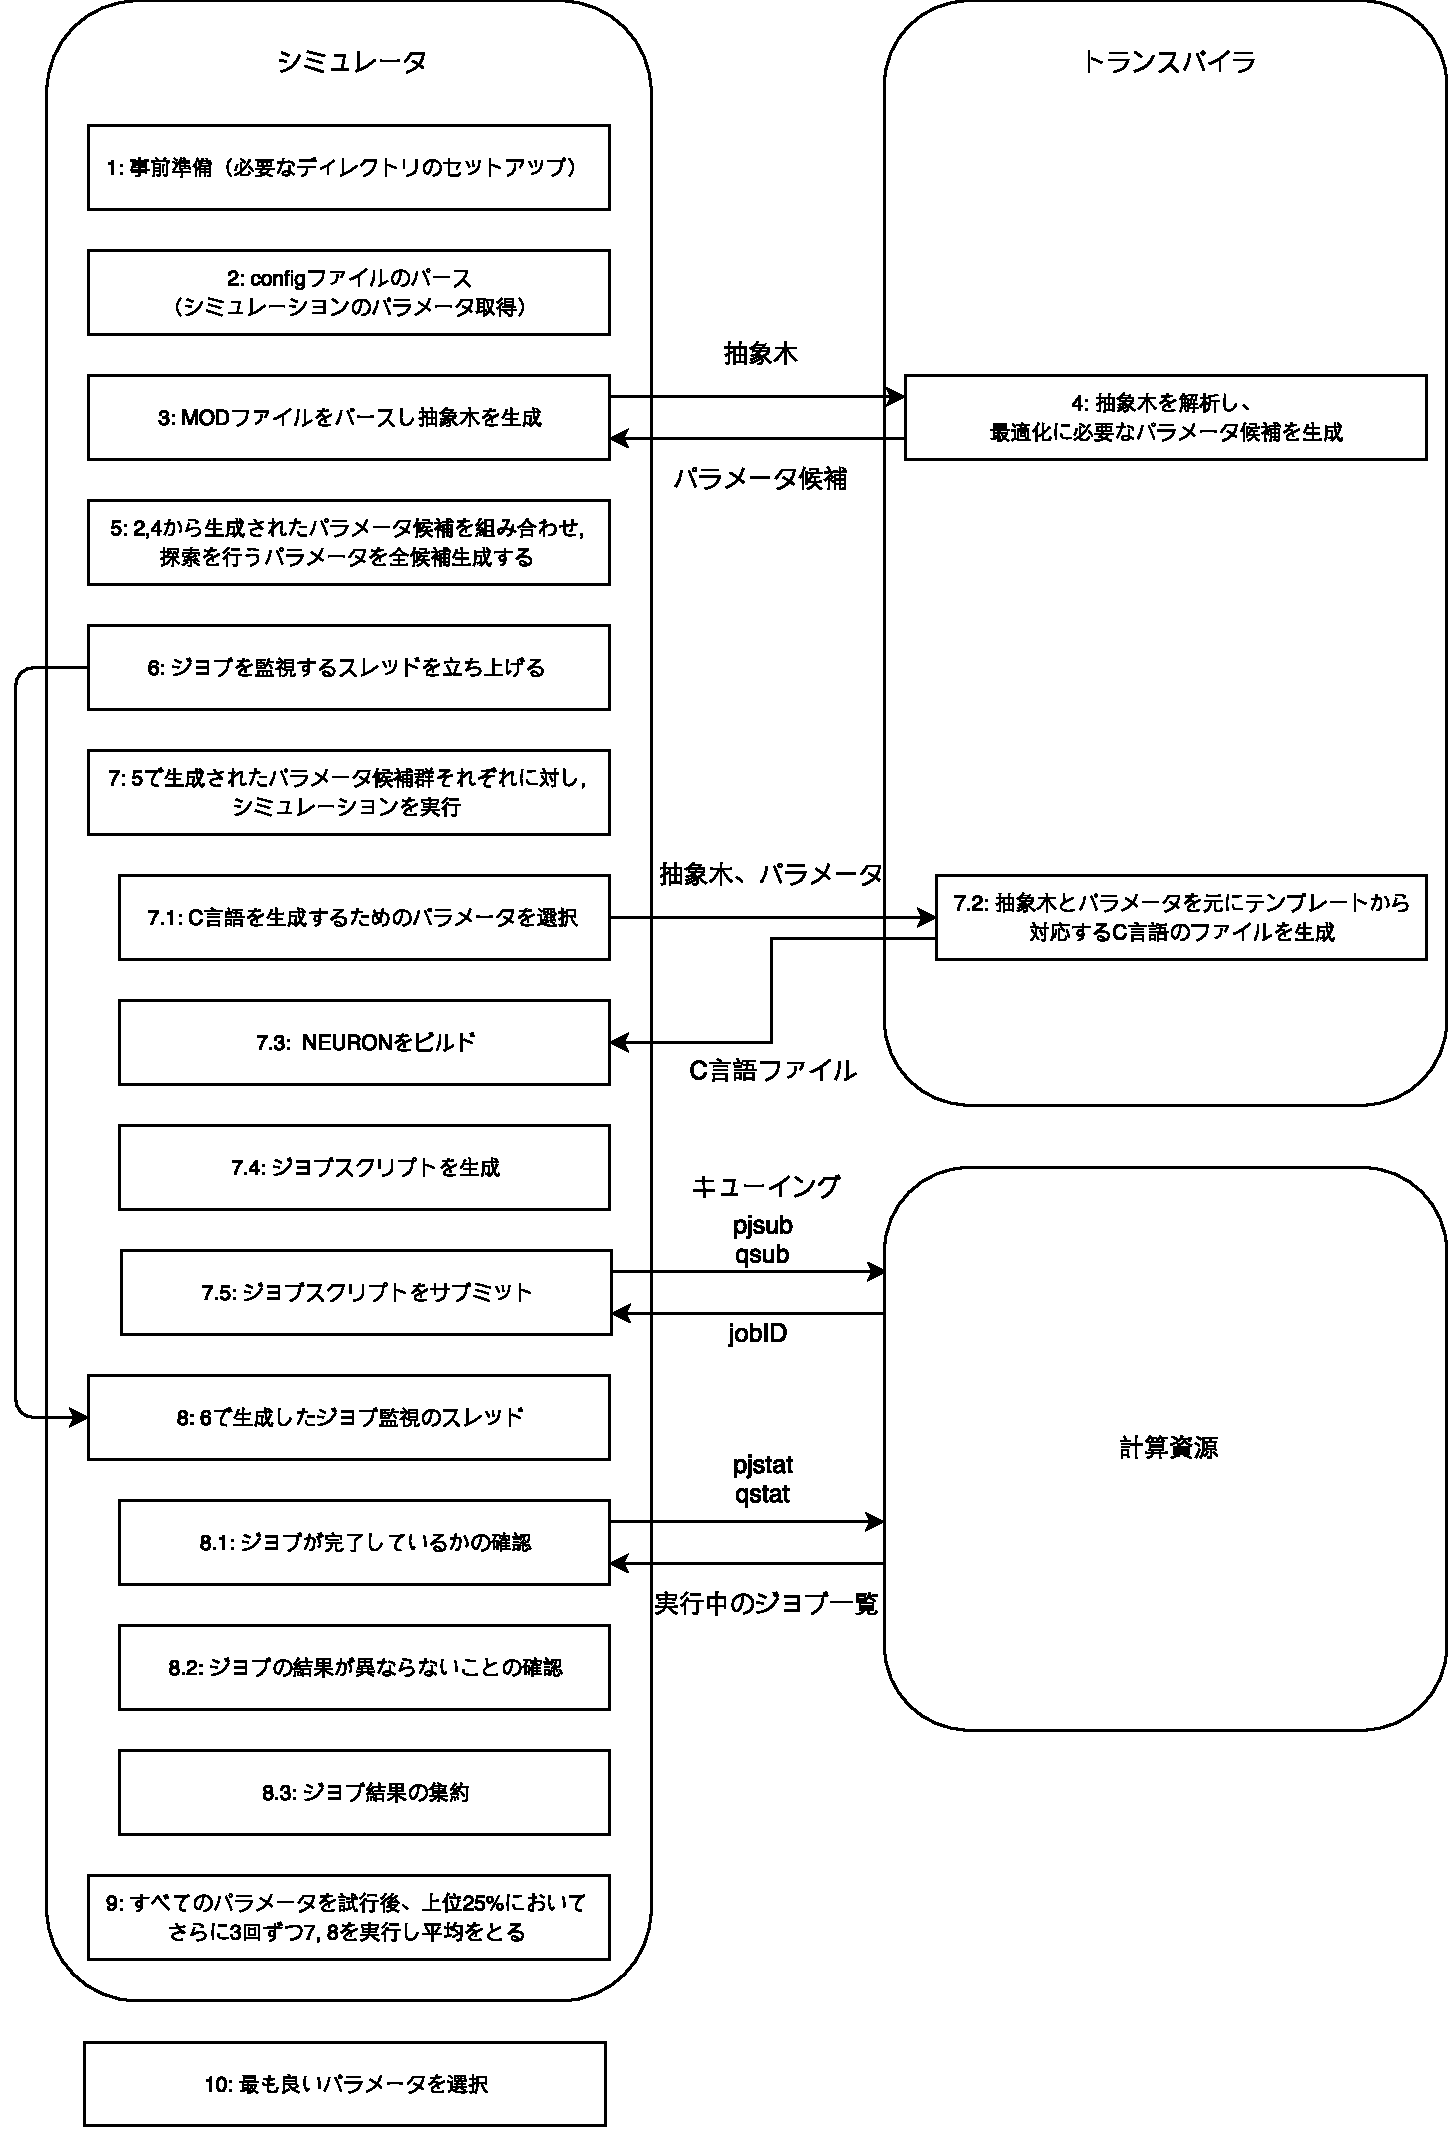
\includegraphics[width=18.0cm]{./images/Genie.pdf}
    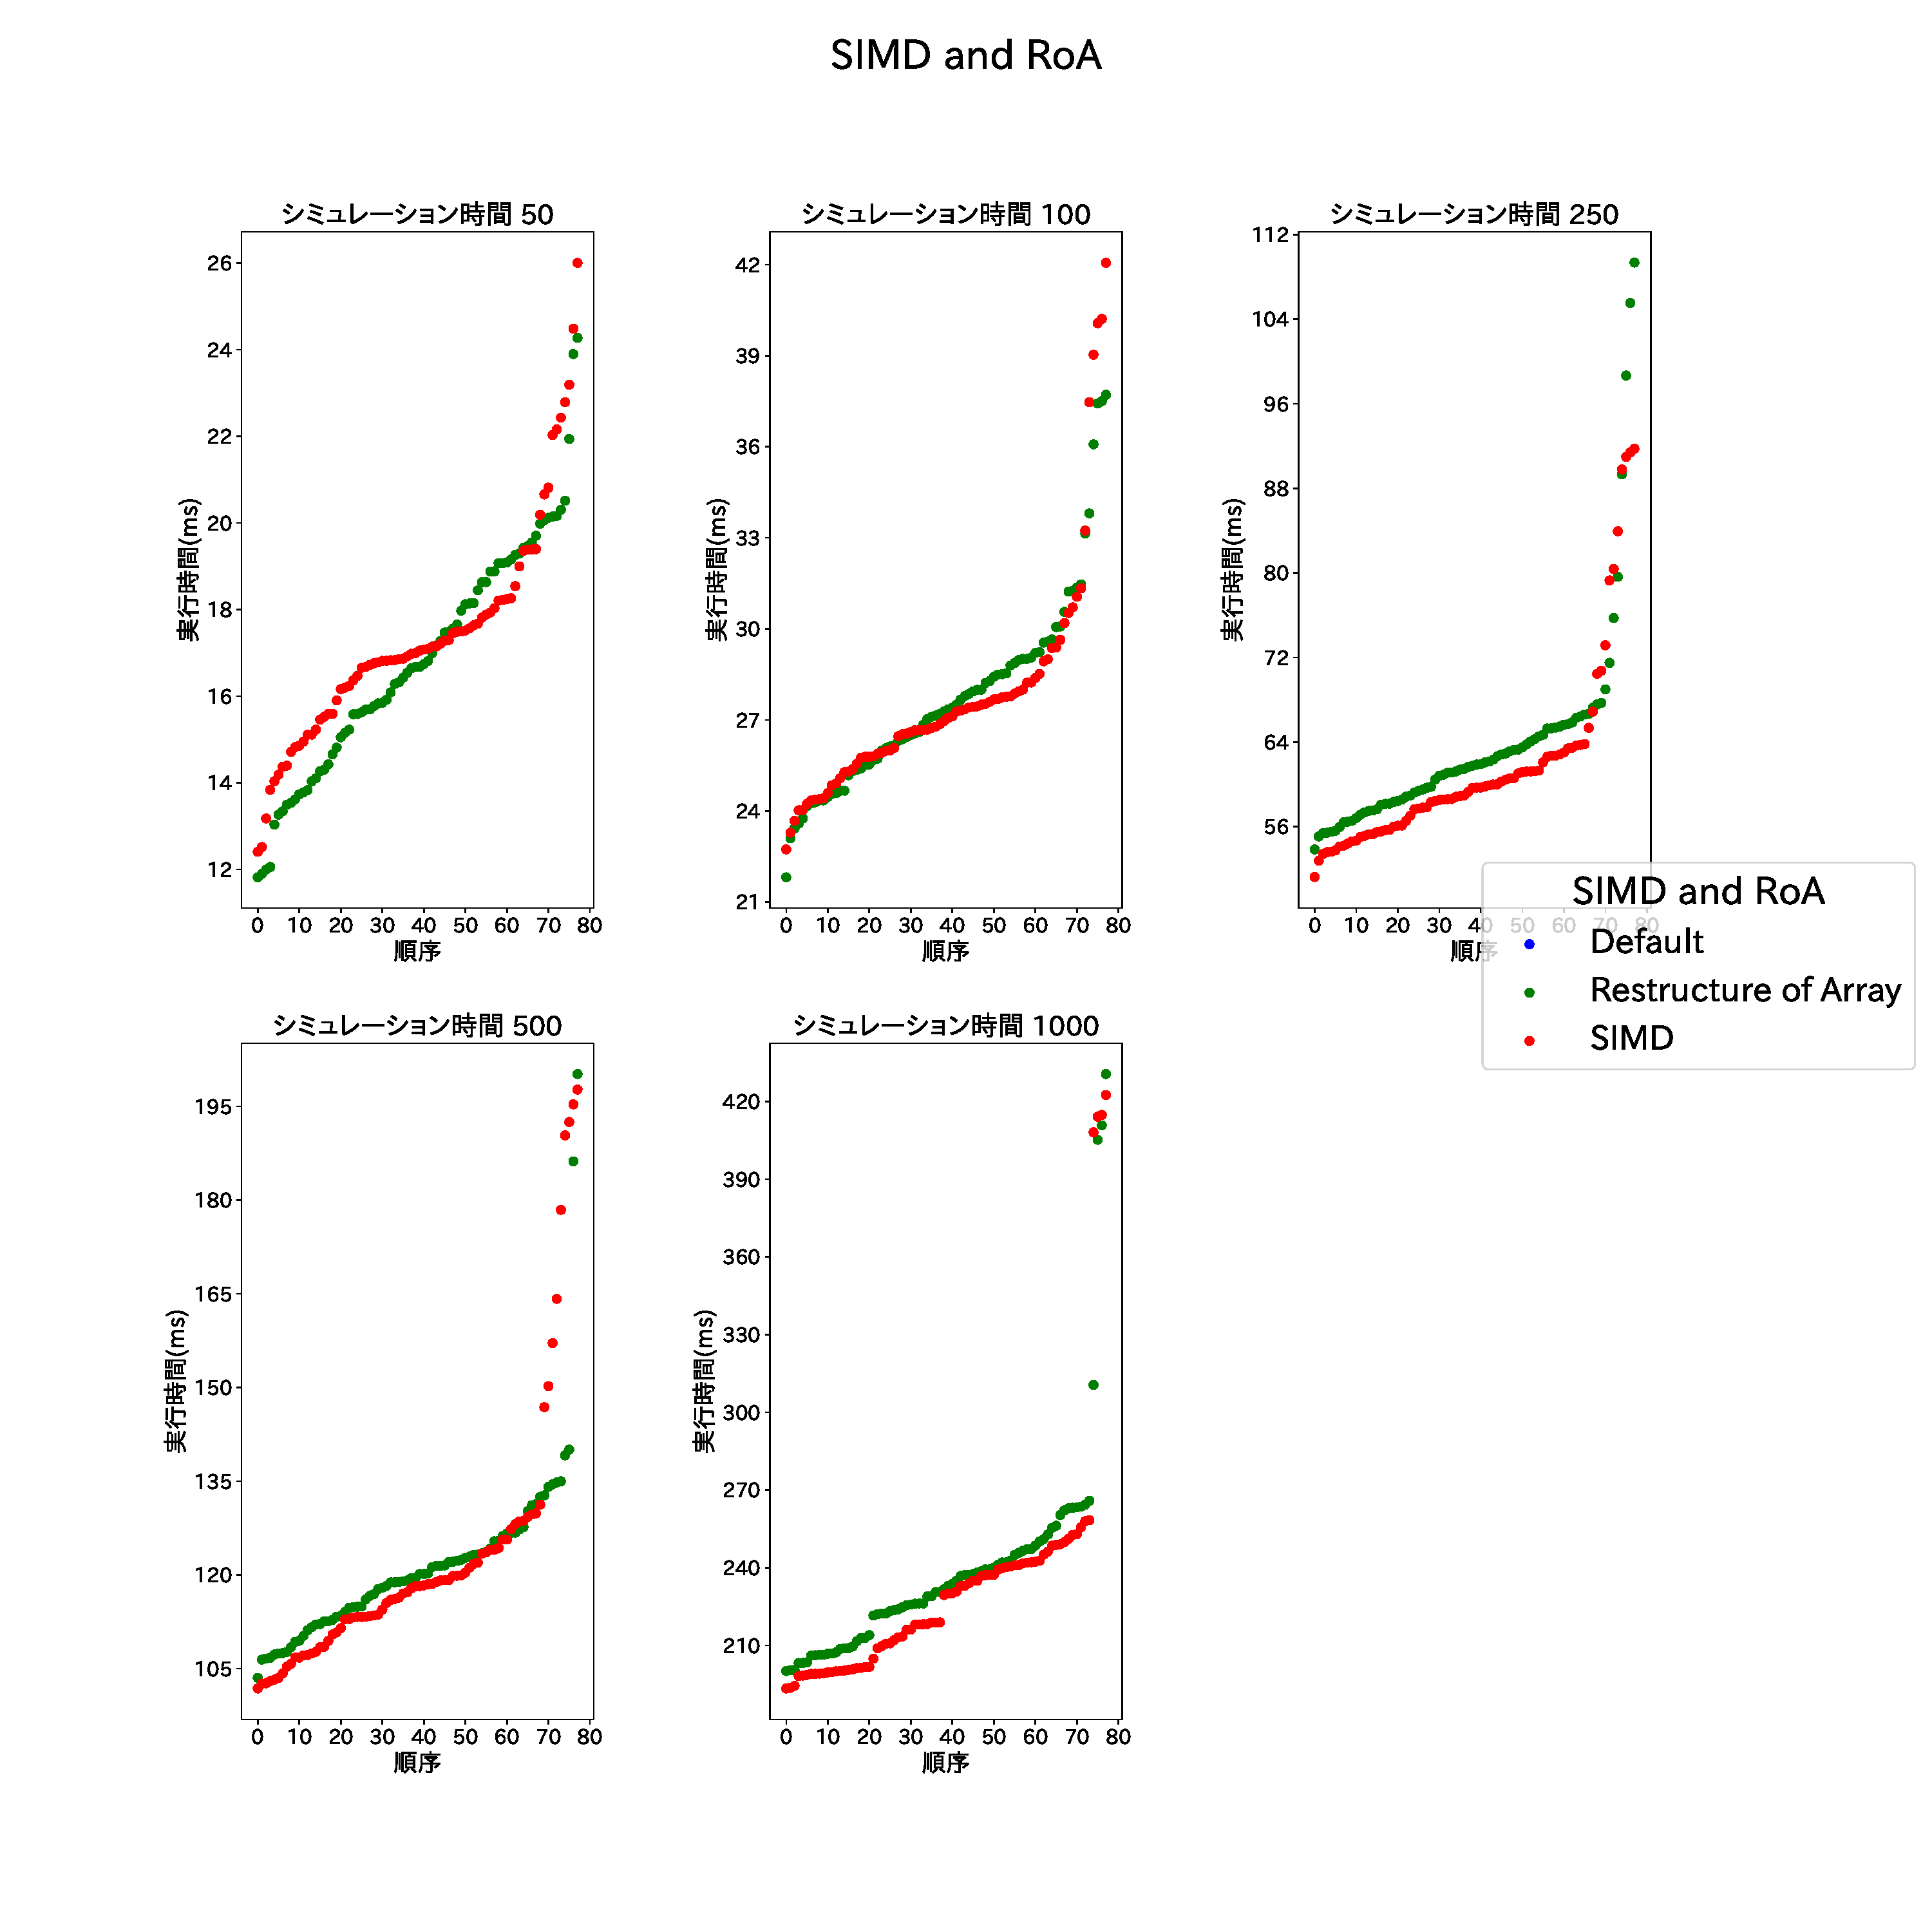
\includegraphics[width=14cm]{./images/cluster-SIMD-and-RoA.pdf}
    \caption{クラスタ 配列のくくり出し シミュレーション結果}
    \label{fig:cluster-roa}
\end{center}
\end{figure}

\begin{figure}[htb]
% h:here, t:top, b:bottom, p:page
\begin{center}
%    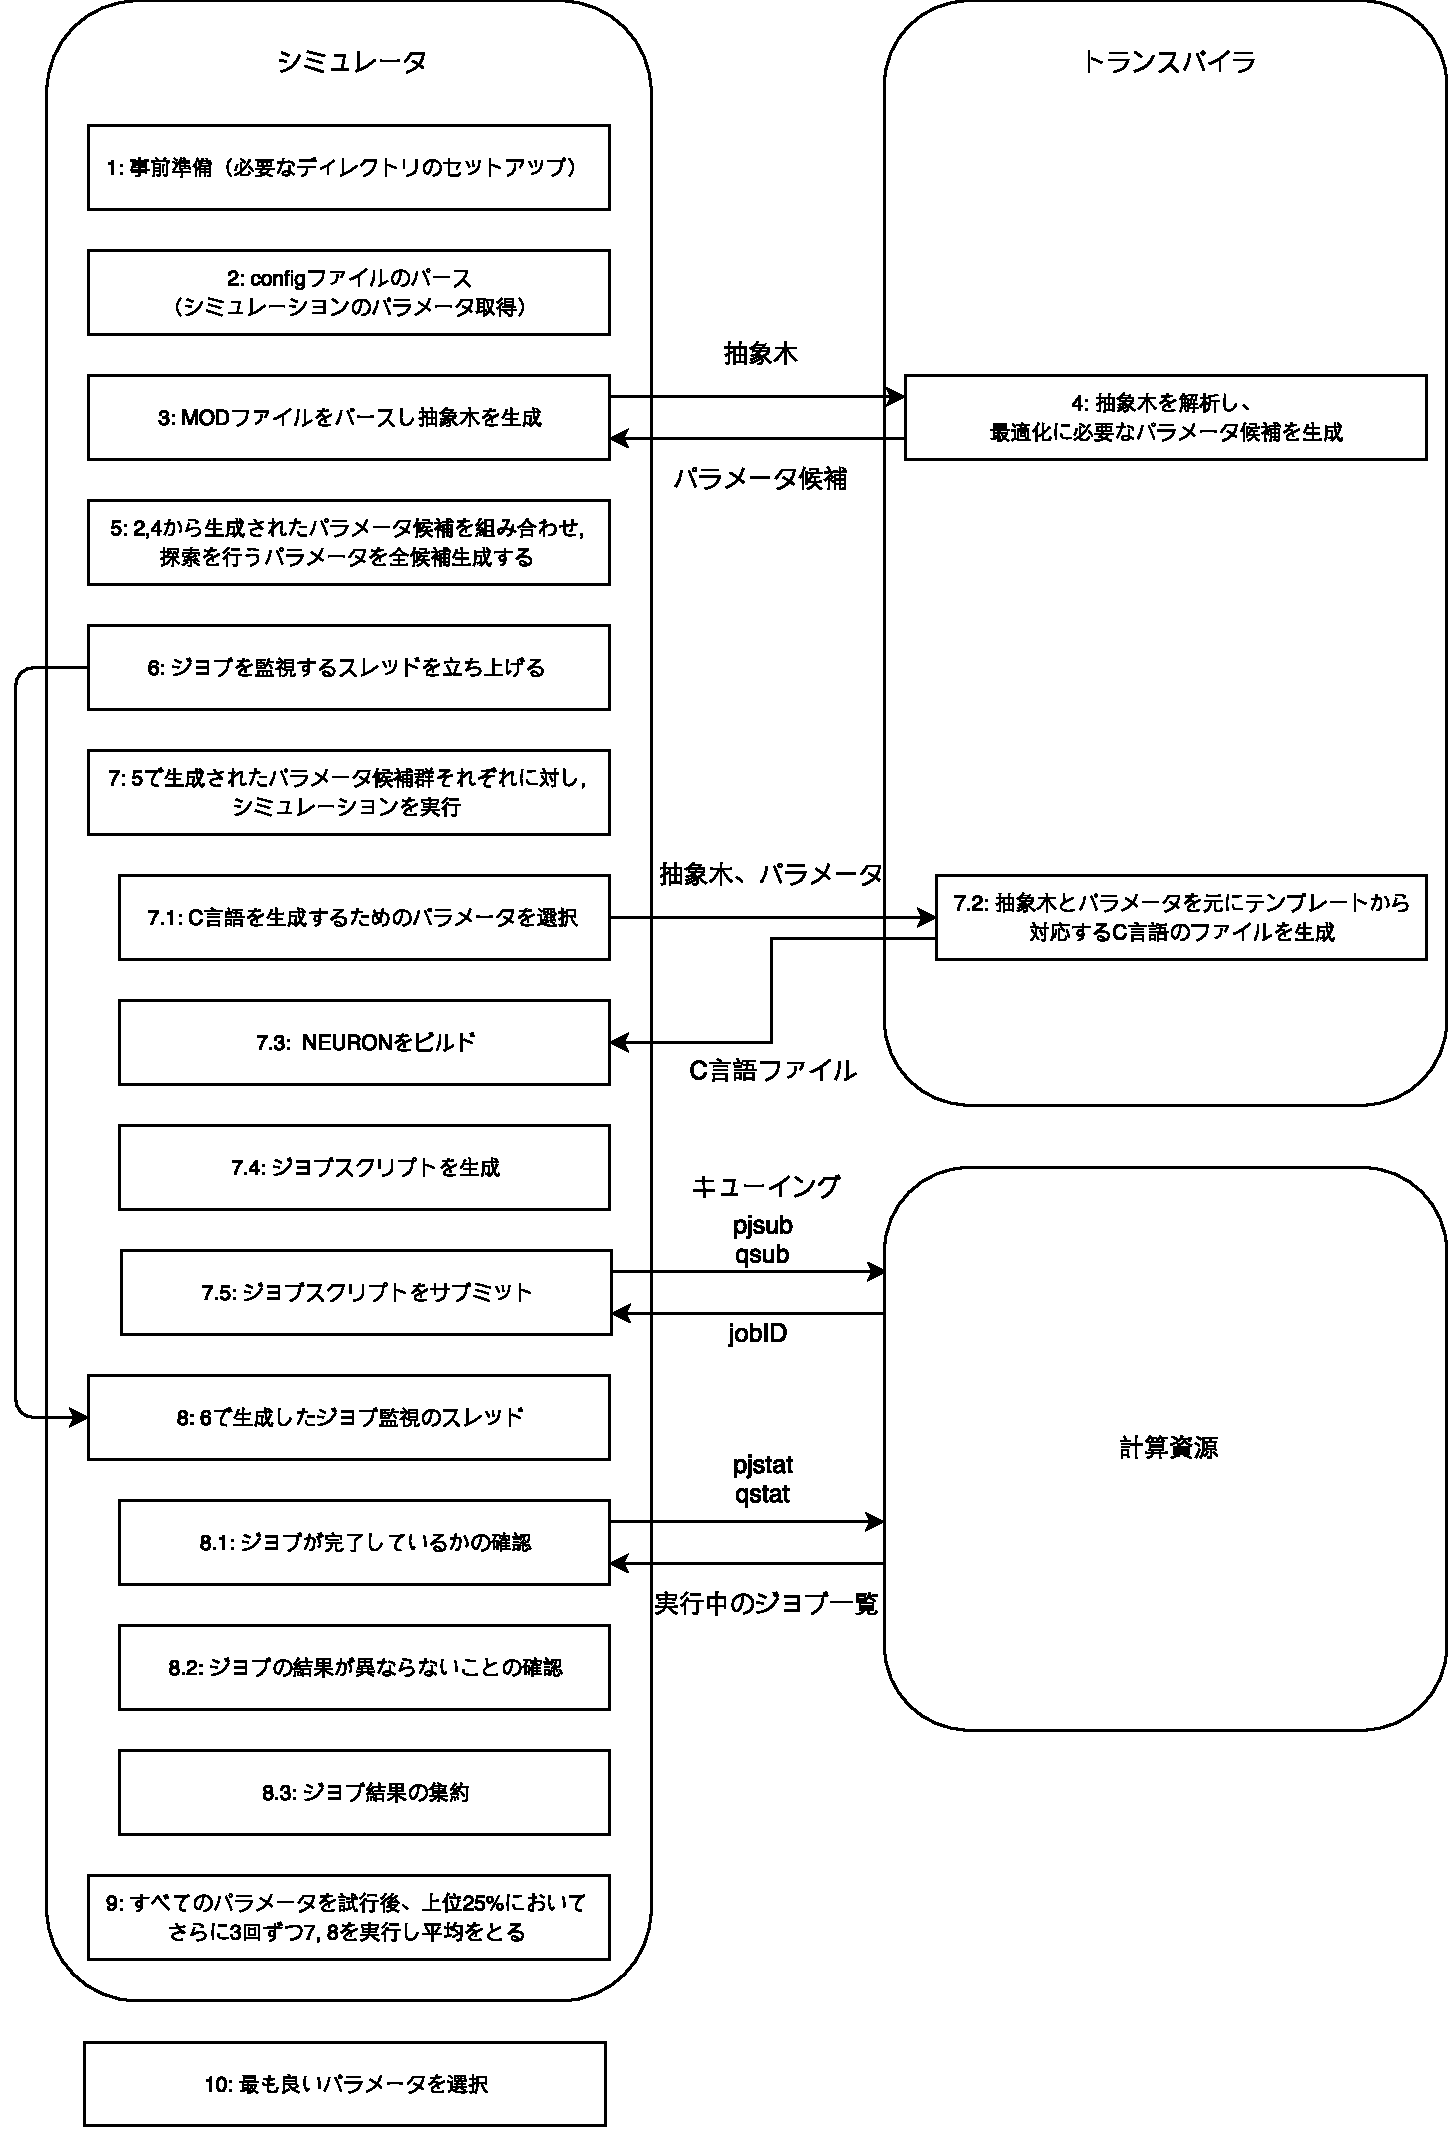
\includegraphics[width=18.0cm]{./images/Genie.pdf}
    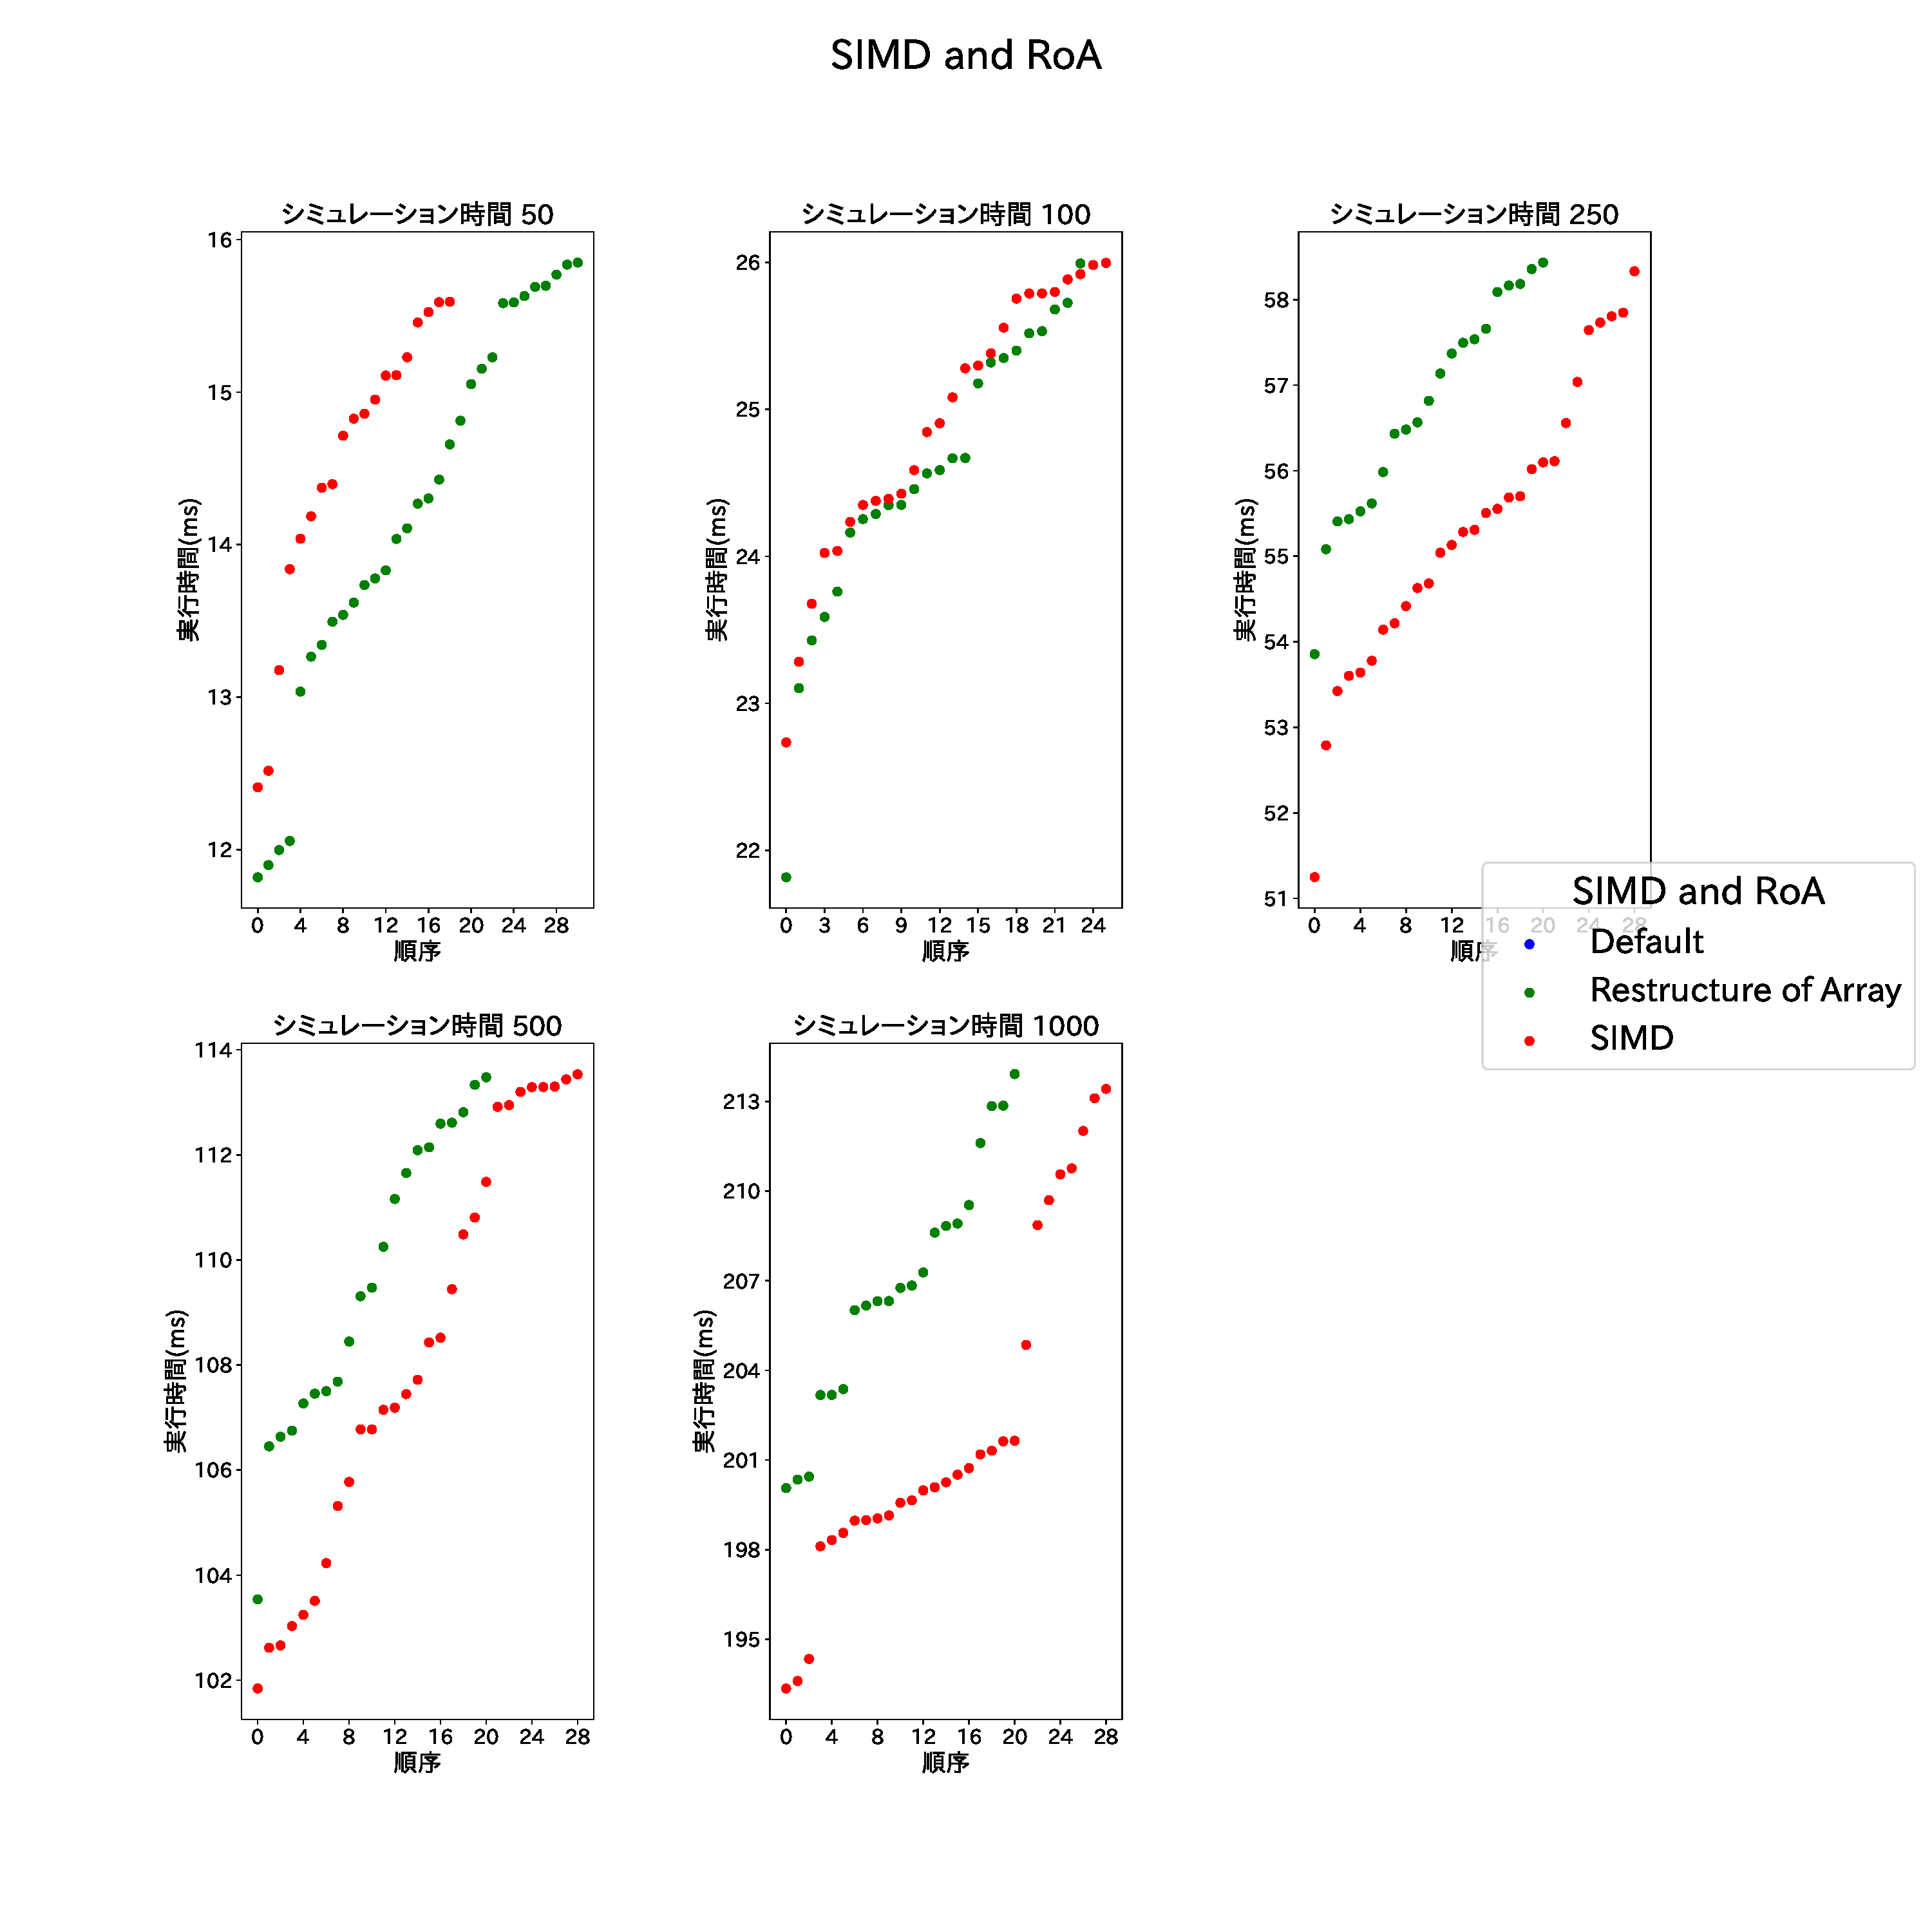
\includegraphics[width=14cm]{./images/cluster-top50-SIMD-and-RoA.pdf}
    \caption{クラスタ 配列のくくり出し シミュレーション結果 上位50組}
    \label{fig:cluster-roa-top50}
\end{center}
\end{figure}
シミュレーション時間が長くなるに連れ,
配列のくくり出しを行わずSIMD化のみを用いたほうが高速化されるように見られるが,
実行時間の差を比較するとシミュレーション時間が倍になった場合でもほぼ一定の差になっているため,
本論文執筆時においての実装では実行時間への影響は少ないことがわかる.\\

\paragraph{京}~\\
% \begin{figure}[htb]
% % h:here, t:top, b:bottom, p:page
% \begin{center}
% %    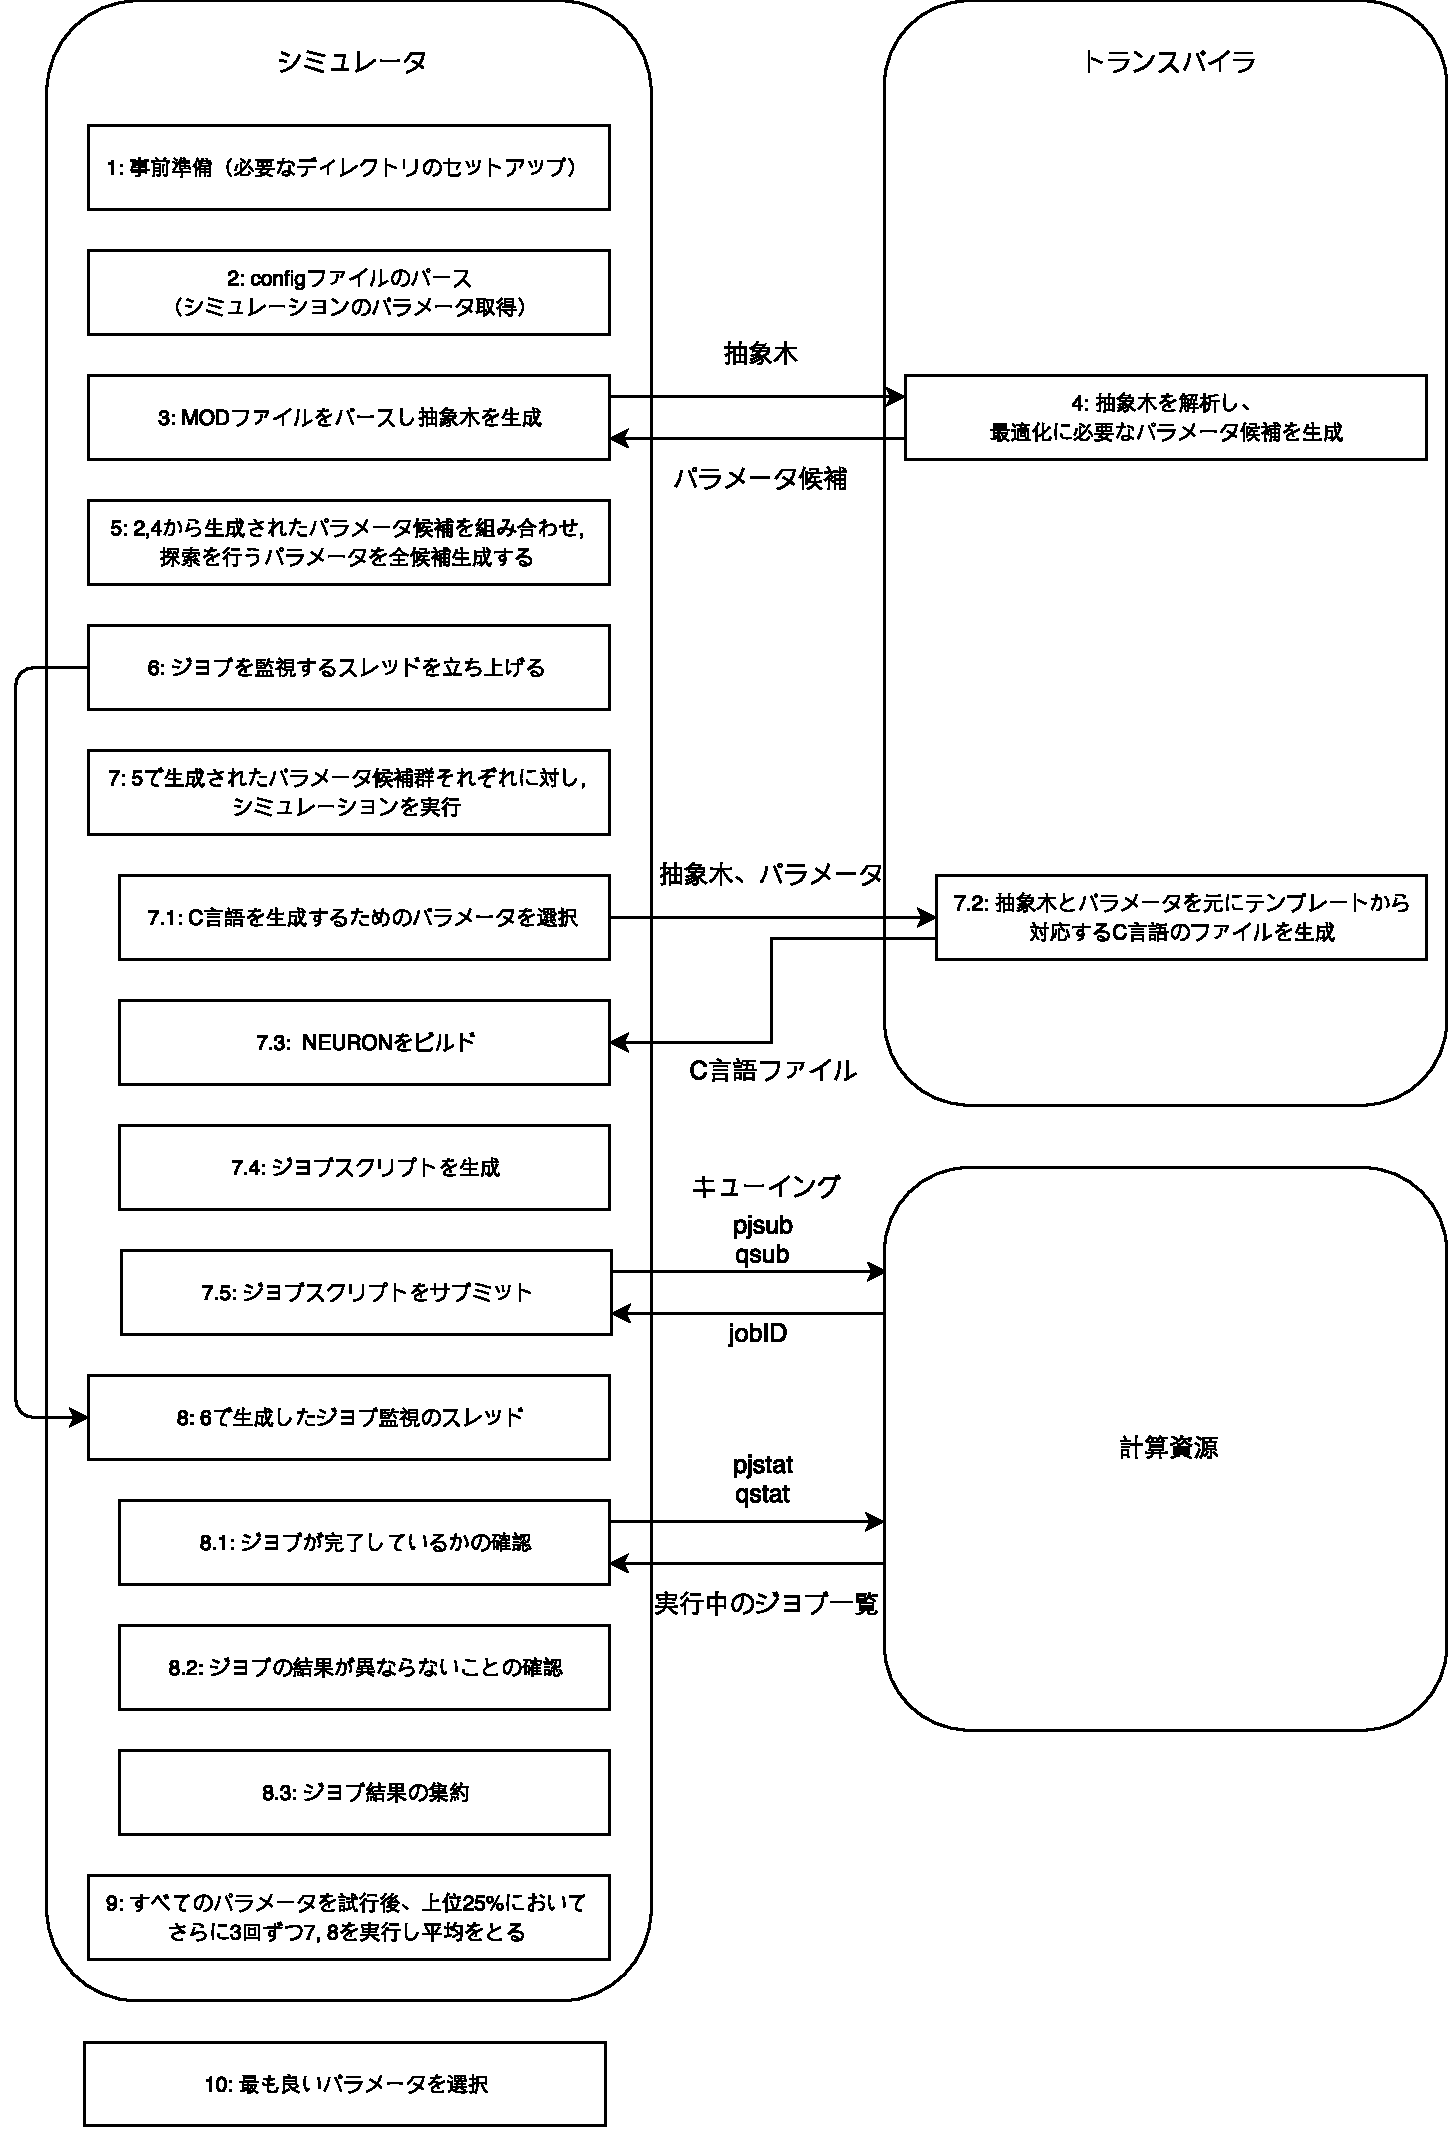
\includegraphics[width=18.0cm]{./images/Genie.pdf}
%     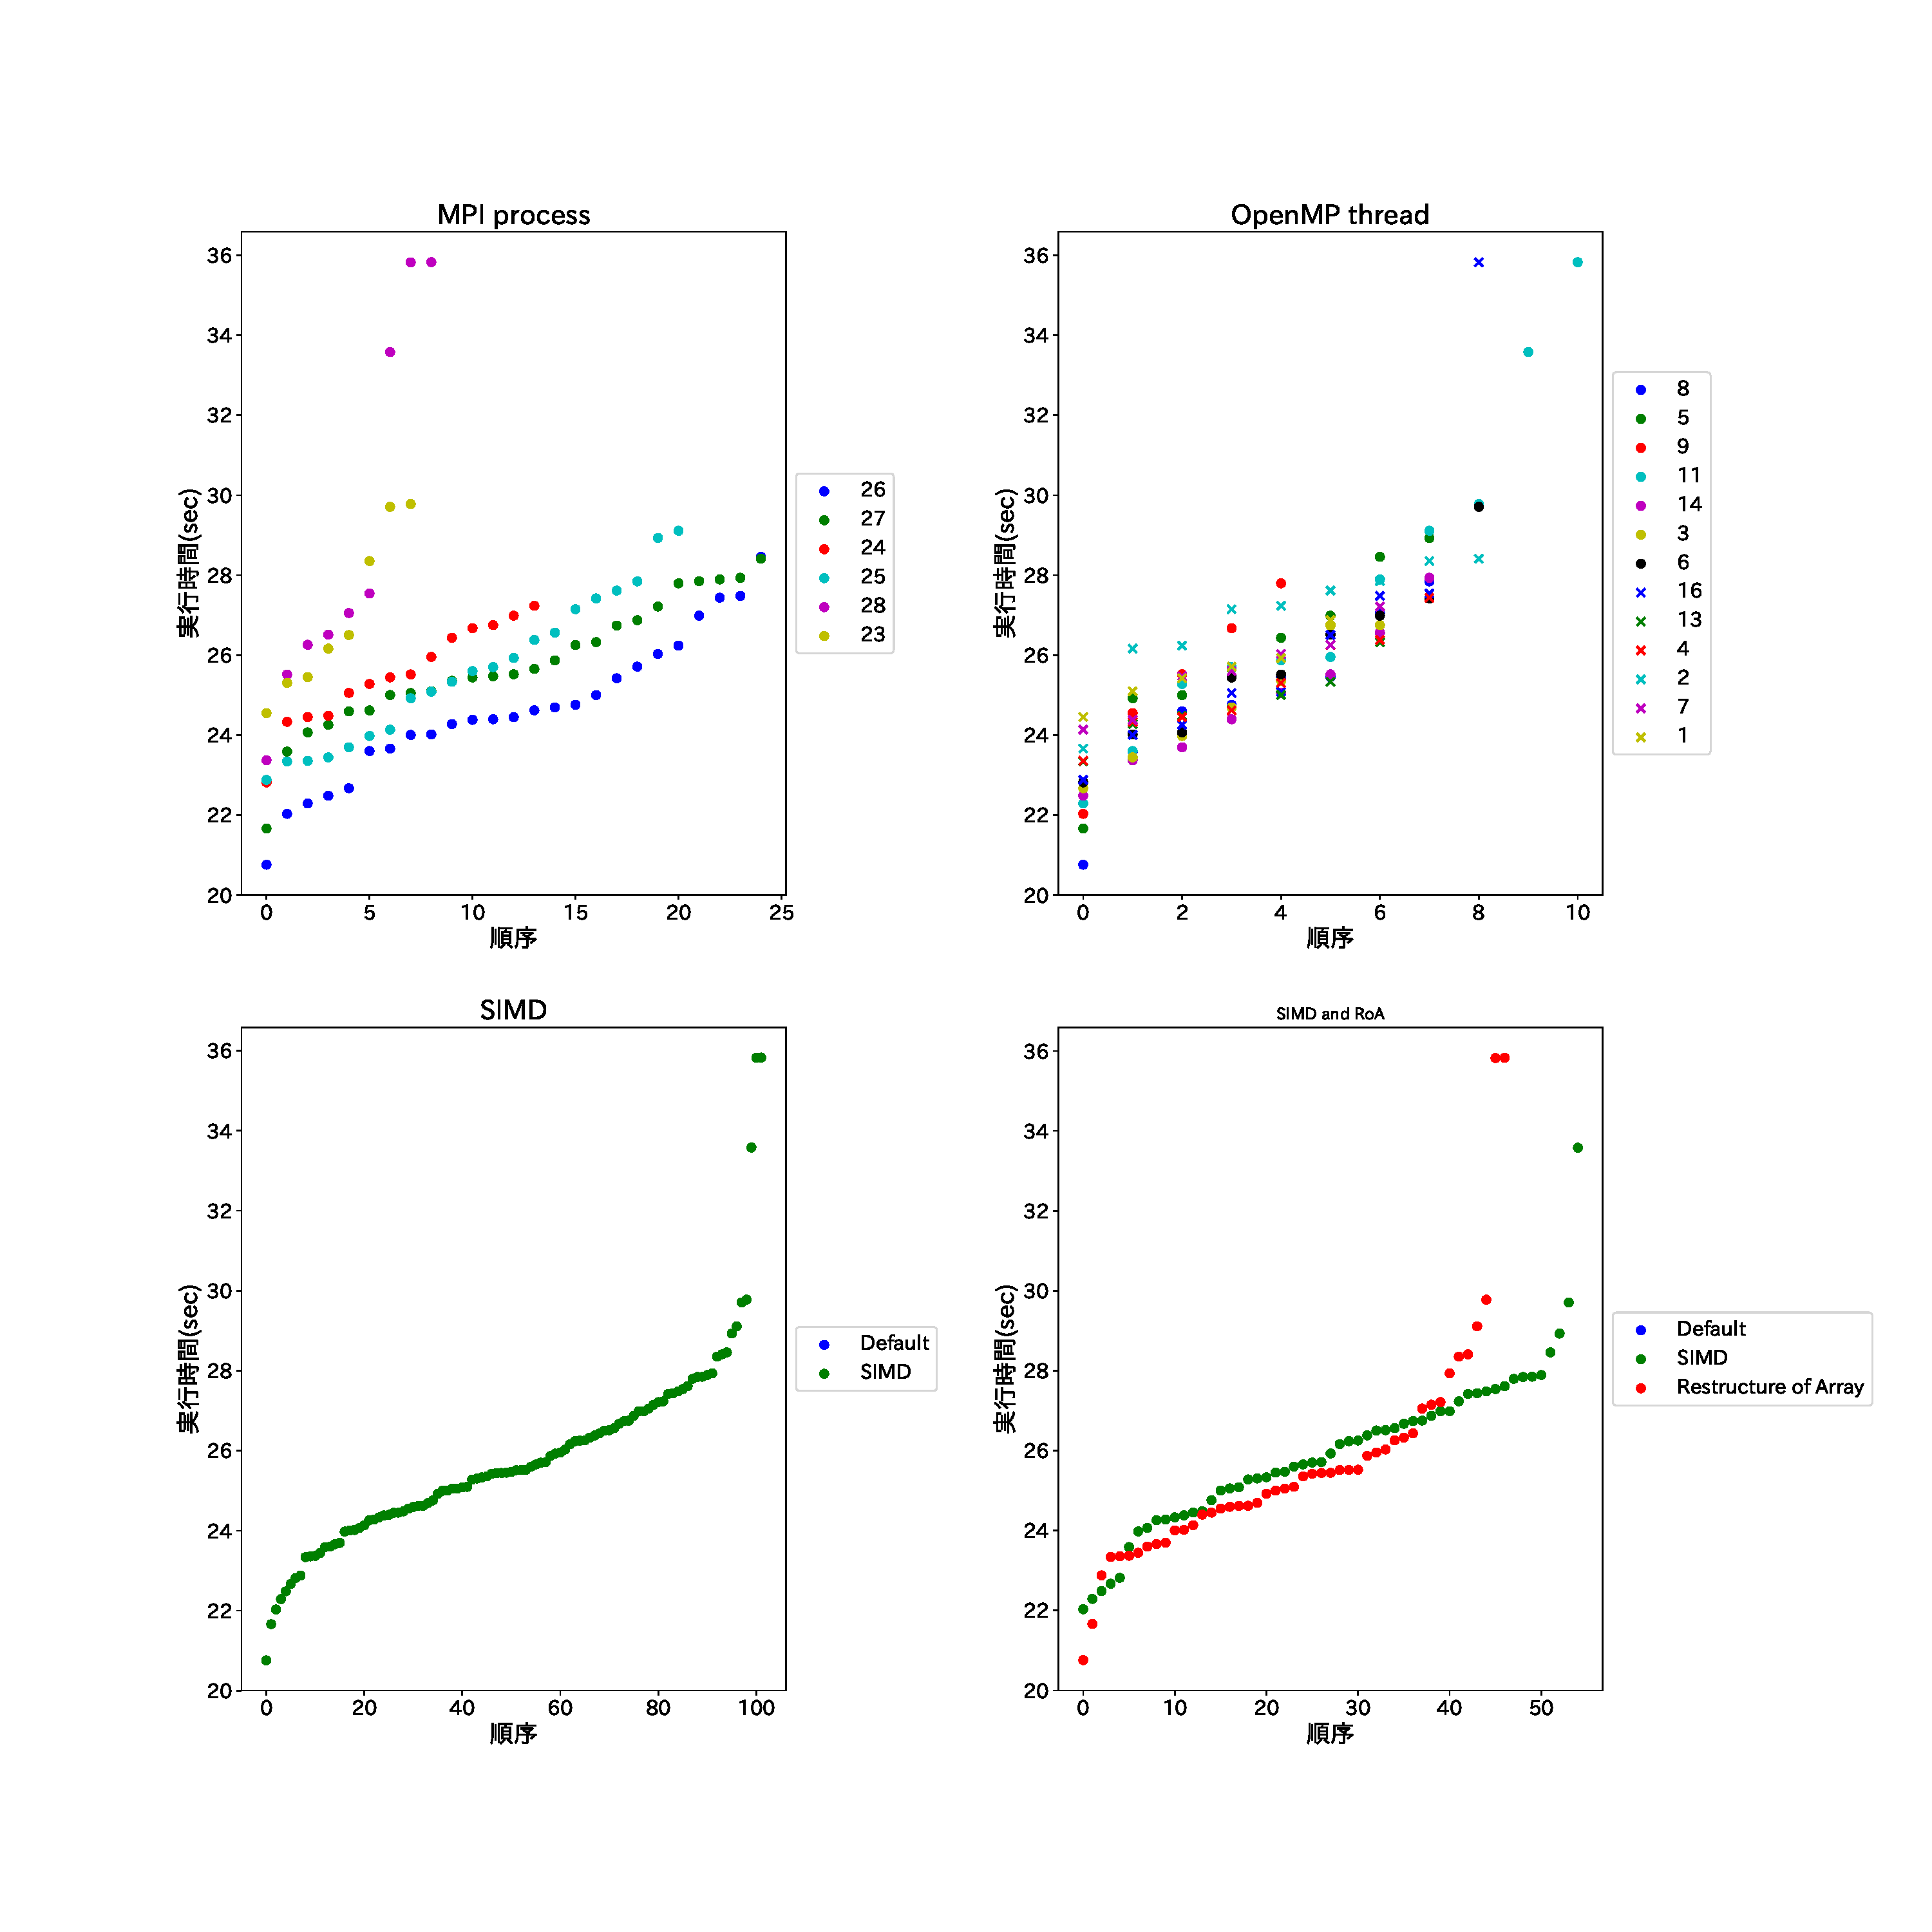
\includegraphics[width=14cm]{./images/cluster-bench-adjusted-final.pdf}
%     \caption{クラスタ 小規模シミュレーション結果 パラメータ絞り込み後}
%     \label{fig:cluster-bench-adjusted-final}
% \end{center}
% \end{figure}
% \clearpage


\section{考察}
% シミュレーション結果を受け手の考察
\section{考察}
\ref{sec:sim-result}章に示したシミュレーション結果について,
その結果から得られた各パラメータとシミュレーションの実行時間について考察する.\\

\subsection{MPIプロセス数とOpenMPスレッド数}
1000msまでのシミュレーションの最適化において, MPIプロセス数は非常に大きな役割を果たすパラメータであったと言える.\\
 クラスタと京双方の環境においてMPIのプロセス数をコア数に近くすることでシミュレーションの高速化がなされたが,
これはハイブリッド並列の仕組み上先にMPIプロセスが生成されたのちにOpenMPのスレッドが生成されるため,
MPIプロセスによってコアを占有することでスレッド生成のコストが抑えられたためであると考えられる.\\
 またこの結果からハイブリッド並列に関与するパラメータは小規模なシミュレーションから求めることはできないということもわかった.
これはMPIプロセスが必要とする通信リソースを小規模なシミュレーションでは使い切れないためであり,
この問題を解決するためには細胞数を現在の256から大幅に増やした状態でのシミュレーションを行う必要があるが,
その場合一度のシミュレーションにかかる時間も比例して大きくなるためパラメータ推定にかかる時間が膨大になるという新たな問題が生じる.\\
 そのためシミュレータの生成するコードやパラメータ推定の方法をより効率化する必要があるが, これは今後の課題としたい.\\

\subsection{SIMD化と配列のくくり出し}
コンパイラによるSIMD化はMPIプロセス数と並び高速化に貢献したパラメータであり,
\ref{subsubsec:simd}項で示した理論値性能とまではいかないもの, 実行時間は半分以上縮まることがわかった.\\
 特に京ではデフォルトのコードとSIMD化を行ったコードとの間で差が大きく出ており, これはSIMD化に強い京コンパイラの貢献が大きいと考えられる.\\
 一方で, 配列のくくり出しに関してはシミュレーションの規模が大きくなるにつれSIMD化のみを行ったものよりも計算性能が落ちているが,
これは配列のくくり出しそのものに意味がないというより,
探索する対象のパラメータの組を減らすため配列のくくり出しを行うか否かの2通りの試行しか行わなかったことが大きな原因であると考えられる.\\
 ゆえに, より多くのパラメータ候補を試行することがそれぞれの最適化アルゴリズムを有効利用するためには必要であり,
ハイブリッド並列化と同様にパラメータ推定の過程そのものを効率化することが詳細な最適化を行う上で必要となると考えられる.\\

\subsection{シミュレーションの規模とパラメータの関係}
一方で, シミュレーション時間100msで行った小規模なシミュレーションにおける各パラメータとシミュレーション時間1000msで行った場合を比較すると,
本研究で用いたパラメータについてはどのパラメータにおいても一定の相関が見られることがわかる.
このことから, 規模を大きくすることで特定のリソースを使い切ってしまうパラメータでないならば小規模のシミュレーションから最適なパラメータ推定を十分に行えると考えられる.\\
 さらに, リソースに関連するパラメータは実行マシンに関わるパラメータであるため,
この事実を利用することでパラメータの候補を実行マシンに関与するパラメータとモデルに関与するパラメータに2分し別々に最適化を行うことも可能であり,
組み合わせによって膨大となっているパラメータ候補数を減らすことが可能であると考えられる.\\

\subsection{本研究の評価}
実行時間という観点では, \ref{subsec:compare}節において示したように本研究で開発したプログラムを利用することで,
手動最適化を行った場合と近い高速化を行えると考えられる.\\
 また, 最適化に用いたパラメータの一つである配列のくくり出しについては探索を行うパラメータの候補が多くなりすぎるという理由で\ref{subsec:small-sim}においては配列のくくり出しを行うか行わないかの2通りのみを対象としていたが,
\ref{subsubsec:soa}で述べたように配列のくくり出しは本来コンパイラによるSIMD化と適切に組み合わせることで効果を持つものである.\\
 そこで附録として, \ref{subsec:compare}節で用いたパラメータのみを対象として, 配列のくくり出しを確かめるべく追加でシミュレーションを行った.\\


\section{結論}


\end{document}
